% !TEX program = xelatex
\documentclass{cumcmthesis}
\let\proof\relax
\let\endproof\relax
\usepackage{amsthm,amsmath,amssymb}
\usepackage{mathrsfs}
\usepackage{graphicx}
%\documentclass[withoutpreface,bwprint]{cumcmthesis} %去掉封面与编号页。
\usepackage{verbatim}  %多行注释
\usepackage{booktabs}    %三线表
\usepackage{multirow}
\usepackage{pifont} 	%序号
\newcommand{\tabincell}[2]{\begin{tabular}{@{}#1@{}}#2\end{tabular}}  %表格过长自动换行
\usepackage[framemethod=TikZ]{mdframed}
\usepackage{url}   % 网页链接
\usepackage{subcaption} % 子标题
\usepackage{colortbl}
%\usepackage{color}
\usepackage{float}
\usepackage{fontawesome}
\usepackage{framed} %framed宏包
\usepackage{tikz}
\usepackage{changepage}
\PassOptionsToPackage{prologue,dvipsnames}{color, xcolor}
\usepackage{graphicx}
\usepackage{ctex}
\definecolor{tabcolor}{RGB}{42, 110, 63} % 这里就是我们怎么定义我们的表格的线宽颜色
\usetikzlibrary{positioning}
\tikzset{>=stealth}

\definecolor{LemonChiffon}{RGB}{255,250,205}

\newcommand{\tikzmark}[3][]
{\tikz[remember picture, baseline]
	\node [anchor=base,#1](#2) {#3};}

\definecolor{grey}{RGB}{220, 220, 220}
\definecolor{darkgrey}{RGB}{170, 170, 170}

% 伪代码
\usepackage[noend]{algpseudocode}
\usepackage{algorithmicx,algorithm}
% 页眉页脚
\usepackage{lastpage}
\usepackage{fancyhdr} % 导入fancyhdr包
\pagestyle{fancy}
% 图表、公式按章节编号
\usepackage{amsmath}
\usepackage{amsfonts,amssymb}
\numberwithin{equation}{section} % 公式按章节编号
\numberwithin{figure}{section} % 图按章节编号
\numberwithin{table}{section} % 表按章节编号
%\setCJKmainfont{Source Han Serif SC} %思源字体
\setCJKmainfont{SourceHanSerifSC-Regular.otf} %思源字体
%\setmainfont{SourceHanSerifSC.otf}
% 设置封面页内容
\titlename{Time-Restricted, Verifiable, and Efficient Query Processing over Encrypted Data on Cloud}
\email{xxx@qq.com}
\yearinput{2025}
\monthinput{0x}
\dayinput{11}
% 页眉设置
\fancyhead[L]{}
\fancyhead[R]{}
\fancyhead[C]{\zihao{-5} Time-Restricted, Verifiable, and Efficient Query Processing over Encrypted Data on Cloud}
% 页脚设置
%\fancyfoot[L]{左页脚}
\fancyfoot[C]{\zihao{-5} 第\thepage 页 \enspace 共 \pageref{LastPage} 页} % 页码
%\fancyfoot[R]{右页脚}
\renewcommand{\headrulewidth}{0.5pt} % 页眉分隔线宽度0.5磅
\definecolor{grayblue}{RGB}{83, 108, 174}
\usepackage{titlesec} %导言区调用titlesec宏包 

\titleformat{\section}{\centering\normalfont\Large\bfseries\siyuan\zihao{3}\color{grayblue}}{第\chinese{section}章}{0.3em}{}	
\titleformat{\subsection}{\normalfont\large\bfseries\siyuan\zihao{4}\color{grayblue}}{\thesubsection}{0.3em}{}
\titleformat{\subsubsection}{\normalfont\normalsize\bfseries\siyuan\zihao{-4}\color{grayblue}}{\thesubsubsection}{0.3em}{}
	
\begin{document}
	
% 将\usepackage{ulem}宏包中的\emph{}还原为斜体
\normalem

% 生成封面页和填写说明页	
\maketitle
 
% 生成目录
\newpage
\thispagestyle{empty}
\tableofcontents
\newpage
 
% 生成图目录
\thispagestyle{empty}
\listoffigures
\newpage

% 生成表目录
\thispagestyle{empty}
\listoftables
\newpage

% 从此处开始编页
\setcounter{page}{1}
 
\begin{cnabstract}
	
    随着云计算的发展,数据存储在云上的比例不断增加,但数据安全和隐私问题也日益突出。传统的加密方法虽然能保护数据安全,但在查询效率和验证结果的正确性方面存在不足。为此,本项目旨在解决云环境中加密数据的安全高效查询问题,提出了一种时间限制的、可验证的、有效的加密数据查询处理方案(TiveQP),其主要功能和特性如下:
    \begin{enumerate}
        \item 时间限制访问:通过将空间属性和时间属性进行编码,支持用户在特定时间范围内访问数据。
        \item 查询结果验证:采用补集验证机制,通过返回比特段和HMAC来验证查询结果的正确性和完整性,而不泄露未查询数据的隐私。
        \item 高效查询处理:设计了剪枝策略,通过分类构建子树来减少不必要的搜索路径,显著提高查询处理速度和结果验证效率。
    \end{enumerate}
    本项目将空间编码技术与时间编码结合,实现了时间限制的加密数据访问控制;提出了补集的概念,通过验证数据项是否在查询范围的补集中,避免了未查询数据的隐私泄露问题;设计了优化的TiveTree索引结构和剪枝策略,显著提升了查询处理和结果验证的效率。
        
    该项目作品具有广泛的应用场景,适用于需要安全查询处理的云存储应用,如医疗数据、金融数据等敏感信息的管理。通过本方案,数据用户可以方便地进行安全查询,并验证查询结果的正确性和完整性,确保数据访问的可靠性。同时,在保证安全性的前提下,显著提高了查询处理速度和验证效率,适应大数据环境下的实际需求,具有很高的实用价值和应用前景。
        
	\cnkeywords{云计算\quad 隐私保护\quad 时空编码\quad 补集验证\quad 查询优化\quad TiveTree索引}
\end{cnabstract}

%英文摘要
\begin{enabstract}
With the development of cloud computing, the proportion of data stored in the cloud is continuously increasing, but data security and privacy issues are also becoming more prominent. Traditional encryption methods can protect data security but have deficiencies in query efficiency and result verification accuracy. To address this, this project aims to solve the problem of secure and efficient query processing for encrypted data in a cloud environment. We propose a time - restricted, verifiable, and efficient encrypted data query processing scheme (TiveQP), which has the following main features:
\begin{enumerate}
    \item Time - Restricted Access: By encoding spatial and temporal attributes, it supports user access to data within specific time frames.
    \item Query Result Verification: Using a complementary set verification mechanism, it verifies the correctness and completeness of query results by returning bit segments and HMAC, without leaking the privacy of unqueried data.
    \item Efficient Query Processing: A pruning strategy is designed, which reduces unnecessary search paths by classifying and constructing subtrees, significantly improving query processing speed and result verification efficiency.
\end{enumerate}
The innovations of this project include combining spatial encoding techniques with temporal encoding to achieve time - restricted access control for encrypted data; introducing the concept of a complementary set, which avoids the privacy leakage of unqueried data by verifying whether data items are in the complementary set of the query range; and designing an optimized TiveTree index structure and pruning strategy, significantly enhancing query processing and result verification efficiency.
    
This project has a wide range of applications, suitable for cloud storage applications that require secure query processing, such as the management of sensitive information like medical data and financial data. Through this scheme, data users can conveniently perform secure queries and verify the correctness and completeness of the query results, ensuring the reliability of data access. At the same time, while ensuring security, it significantly improves query processing speed and verification efficiency, meeting the practical needs of big data environments, and has high practical value and application prospects.
    
\textbf{Keywords}: Cloud Computing; Privacy Protection; Spatio - temporal Encoding; Complementary Set Verification; Query Optimization; TiveTree Index;
\end{enabstract}
% \textcolor[rgb]{0.235,0.502,0.717}{\section{作品概述}}

\section{作品概述}
% 蓝色 60 113 183

本章分为背景分析、相关工作、研究问题、特色描述与应用前景分析五个部分,旨在对本时间受限可验证查询方案系统进行整体的介绍。

\subsection{背景分析}

在数字化浪潮席卷全球的当下,云计算与位置服务(LBS)的深度融合正重塑人类社会的运行逻辑。截至2025年,全球云计算市场规模突破7,000亿美元,LBS日活用户超50亿,支撑着从实时导航到元宇宙空间定位的多元化场景。然而,技术赋能的另一面是愈发尖锐的隐私博弈——用户的位置轨迹、行为偏好等数据成为商业竞争与国家安全的新战场。苹果公司2024年推出的“私密云计算”(PCC)技术,通过无持久存储设计、硬件加密密钥随机生成及算后即焚机制,为云端AI处理构建了封闭的隐私保护屏障,其服务器操作系统经第三方审计验证,确保数据无法被追溯至具体用户。这一创新既是对传统云服务架构的颠覆,也映射出行业对隐私保护的技术焦虑。

全球数据主权意识的觉醒正催生严苛的监管矩阵。欧盟《人工智能法案》(2024生效)首次将LBS算法偏见纳入审计范围,要求公开数据处理逻辑的可解释性;中国《个人信息保护法》则通过芯片级可信计算强化全链条安全要求。跨国公司深陷合规泥潭:Meta因违规迁移欧盟用户数据被罚12亿欧元,暴露全球化服务与本地化立法的根本冲突;滴滴出行因未审计行程数据共享触发监管下架,凸显企业内部控制的系统性风险。这种监管与技术之间的张力,在跨境数据流动中尤为显著——美国CLOUD法案与欧盟GDPR的管辖权冲突,迫使企业采用“数据本地化孤岛”策略,但由此产生的运营成本与技术碎片化正成为数字经济的新桎梏。

技术防御与攻击的“军备竞赛”已进入量子级对抗阶段。传统加密体系在IBM量子计算机的威胁下岌岌可危,后量子加密算法成为云服务商升级焦点。微软Azure SQL Database通过同态加密实现毫秒级加密态检索,阿里云则构建三级认证体系,从基础知识到高级应用覆盖全链条安全能力。值得警惕的是,攻击手段正从数据窃取转向时空关联分析——2024年英国NHS新冠追踪APP因哈希算法缺陷导致用户身份反推,揭示匿名化技术在行为模式识别中的脆弱性。这种风险在元宇宙场景中呈指数级放大,IDC预测2030年XR设备位置数据达80ZB,虚拟空间的行为轨迹可能成为现实身份破解的密钥。

未来十年,隐私保护范式将经历从“数据控制”到“算法治理”的范式迁移。苹果PCC技术中“透明日志验证”机制,华为云的三维点云定位专利,均指向算法透明度的新战场。当瑞士SkyMedical急救无人机通过保形加密技术兼顾3秒响应与位置隐匿,当马士基物流区块链用零知识证明验证货物真实性,我们看到的不仅是技术突破,更是隐私、效率与成本“不可能三角”的突围尝试。这场关乎数字文明基石的博弈,终将在量子计算与元宇宙的叠加效应中,书写新的技术伦理篇章。

\begin{figure}[h]
	\centering
	
\includegraphics[width=1.0\linewidth]{ jpgs/电信诈骗.png }
	\caption{ 关于防范和打击电信网络诈骗犯罪的通告 }
	\label{关于防范和打击电信网络诈骗犯罪的通告}
\end{figure}

\subsection{相关工作}
本节将回顾安全 \(k\) 近邻(SkNN)查询处理和隐私保护范围查询处理的相关研究。

\textbf{\bfseries\siyuan{(1)SkNN 查询处理}}

雷等人 \cite{18} 提出了一种名为 SecEQP 的安全高效查询协议。该协议通过一组基础投影函数将位置转换为多个可行区域,再将这些区域整合成不规则多边形。云服务器通过对比两个位置的复合投影函数输出代码是否相等来判断其接近程度,并将代码存入不可区分布隆过滤器(IBF)构建 IBF 树。数据用户生成投影函数代码作为查询令牌,云服务器通过搜索 IBF 树完成查询。但该方案无法实现结果验证。

崔等人 \cite{19} 设计了可验证的安全 \(k\) 近邻协议 SVkNN。该方案采用 Voronoi 图划分区域,通过可验证安全索引(VSI)支持快速查询验证。虽然提出了紧凑验证方法,但需依赖双服务器架构,导致额外的计算和通信开销。我们认为,大多数用户仅需在常规区域进行查询,无需处理复杂形状区域(如不规则多边形和 Voronoi 单元),且现有方法需用户预处理整个区域,效率较低。因此,本文设计了一种轻量级空间编码技术,以减少用户预处理时间和服务器索引搜索时间。

\textbf{\bfseries\siyuan{(2)隐私保护范围查询处理}}

李等人 \cite{20} 首次提出支持选择关键字攻击下索引不可区分的范围查询协议。该方案通过前缀编码转换数据项,将哈希随机化后的前缀存入布隆过滤器构建 PB 树。用户将查询范围转换为最小前缀集生成陷门,服务器通过搜索 PB 树匹配查询。在此基础上,李等人 \cite{21} 进一步提出支持联合查询的隐私保护协议,采用孪生布隆过滤器(IBF)实现自适应安全,并构建 IBF 树替代传统 PB 树。

吴等人 \cite{22} 提出的 ServeDB 协议支持加密数据多维范围查询,通过树索引验证机制确保结果正确性。但该方案返回的验证证明包含叶节点布隆过滤器,可能导致用户通过布隆过滤器查询其他范围,造成隐私泄露问题。

\subsection{研究问题}

在\texttt{SNN}框架下处理云位置数据时,面临着一系列挑战:

(1)首先,在处理云位置数据时,一个迫切需要解决的问题是如何有效地应对用户对时间限制访问的需求。传统的位置查询服务往往只考虑了空间距离,但随着用户需求的不断演变,例如需要在特定时间范围内获取信息,这种情况变得越来越普遍。因此,我们需要探索如何在位置查询中集成时间限制,以便向用户提供更精确和个性化的服务。这需要在云计算数据处理中引入更多复杂性,并且需要设计和实施新的算法和技术来满足这种需求。

(2)其次,在处理云上位置数据时,保护数据所有者和用户的隐私是一个至关重要的问题。位置数据涉及用户的日常活动、行为习惯甚至健康状况等敏感信息。因此,确保这些数据不被未授权的访问或滥用至关重要。为了解决这一问题,需要采取一系列的隐私保护措施,包括数据加密、访问控制和隐私保护协议的设计。

(3)尽管现有的位置查询方案可能具有一定的结果验证性,但在保护隐私方面仍然存在着不足之处。用户可能通过分析查询结果来获取未查询数据的隐私信息,从而导致数据泄露和隐私侵犯的风险。因此,我们需要设计更加严格和可靠的隐私保护机制,确保即使在验证结果的过程中也不会泄露用户的隐私信息。这涉及到使用更加安全的加密算法、隐私保护技术的创新以及强化隐私保护协议的实施等方面。

(4)最后,当前的位置查询方案往往忽视了数据项的空间属性,导致了查询效率的下降。然而,通过充分利用空间属性,可以设计出更加高效的查询处理方法,从而提高系统的整体性能和用户体验。这涉及到设计新的数据结构和算法来处理空间属性、优化查询处理过程以减少查询时间,以及引入更加智能化的查询优化策略等方面。通过这些措施,我们可以更好地应对处理云上位置数据时面临的挑战,并提高系统的整体性能和用户满意度。

为解决上述问题,提出的方案是\texttt{TiveQP}方案。\texttt{TiveQP}方案旨在解决位置数据隐私问题,特别是针对基于位置的服务中的隐私保护时间限制访问,与现有的\texttt{SNN}隐私和隐私保护范围查询方案相比,\texttt{TimevQ}方案具有三个主要优势:(1)支持隐私保护时间限制访问;(2)采用更强的威胁模型实现隐私保护结果验证;(3)通过利用属性提高查询效率。通过这些优势,\texttt{TimevQ}方案能够更好地满足数据所有者和用户的需求,提供更安全和高效的位置服务。为了达成这些目标,我们的项目方案面临着以下三个挑战:

\textbf{\bfseries\siyuan{如何实现具有安全的时间限制访问的\texttt{SNN}查询处理?}}空间转换和编码技术通常用于解决位置查询问题。安全的时间限制访问本质上是一个隐私保护的范围查询问题。一种直接的方法是分别处理空间属性和时间属性。然而,这样做会导致效率低下。我们必须将这两个问题整合起来,并统一执行查询。为了解决这个问题,我们使用空间编码技术来处理位置,并利用前缀编码来处理位置和时间,将所有生成的数据项的码都投影到一个不可区分的布隆过滤器(\texttt{IBF})中。即,一个整合索引。每个查询都被编码成一组密钥门。通过这种方式,我们将这两个问题整合起来。

\textbf{\bfseries\siyuan{如何在现有的\texttt{SNN}框架下实现结果验证而不违反结果隐私?}}这个领域的开创性论文是\texttt{ServrDB}[7],作者提出了一种有效的方法,可以验证其结果的正确性和完整性,而不需要引入新的结构。对于完整性,云服务生成与数据用户发现每个步骤相关的搜索路径的证明信息。不幸的是,一些关键点,即叶节点,包含在返回的证明中。这允许数据用户在节点上自由查询任何集合,从而违反了未查询数据项的隐私。为了解决这个问题,我们提出了零知识集的概念,我们不证明值位置不在区域\(A\)中,而是证明它位于\(A\)的补区域中。具体来说,数据所有者为每个数据项计算了位置、类型和开放时间的三个补集合。每个集合都转换为最小的前缀集合。每个前缀都被查询节点\texttt{IBF}中生成一系列比特段。此外,对比特段计算出一个带有哈希的哈希消元返回码(\texttt{IMAC})作为签名。当证明与匹配时,我们将匹配的比特段及其\texttt{IMAC}返给数据用户,而不是返整个\texttt{IBF}段。

\textbf{\bfseries\siyuan{如何在概率性安全性的情况下进一步提高查询效率?}}在概率性安全性的前提下提高查询效率是一项艰巨的任务[19],[5]。为了提高效率,在创建索引的操作\texttt{TimevQ}时,我们设计了一种修剪策略,首先根据它的空间属性(例如类型和城市)对数据项进行分类,然后从底部向上为每种类型的位置构建子树。通过这样做,我们消除了不必要的搜索路径,减少了查询处理时间和结果验证时间。查询复杂性降低到 $\mathbf{O}(k\log(\frac{n}{t\times c}))$,其中 $t$ 和 $c$ 分别是类型和城市的数量。

subsection{特色描述}
我们提出的解决方案 \texttt{TiveQP}(时域受限可验证高效查询处理,Time-Restricted, Verifiable, and Efficient Query Processing over Encrypted Data on Cloud),能够在云环境中抵御恶意云服务器的攻击,使得数据用户可以在不泄露其查询内容和位置隐私的情况下进行高效的查询和数据处理。系统架构如图1所示,包含三个核心实体:

(1) 扩展 SKNN 的时间受限查询。TiveQP 系统的第一个特色是扩展了传统的安全 k 最近邻(Secure k Nearest Neighbor, SkNN)查询,允许用户在特定时间段内查询 k 个最近的位置。这种时间受限的访问控制对用户来说非常重要。我们假定由一位患者需要医院的主刀医生,那么这位患者在提供地点信息外还要加上时间限制,预约医生的空闲时间段。

(2) 安全抵抗强化威胁模型。TiveQP 采用了更强的威胁模型来验证自身的安全性。在这种假设的强化威胁模型中,云服务器 (CS) 是恶意的。即安全系统不仅需要抵抗来自外界的攻击还要防范来自云服务器的可能窃取。但在 TiveQP 模型下,数据用户仍然可以验证查询结果的正确性,而不会泄露未查询的数据项的信息。这种安全性是通过补集验证技术实现的,即证明某数据项“在”某集合中的方式被转化为证明其“在”补集中。TiveQP 模型的安全性也得以增强。

(3) 高效查询和验证。为了提高查询处理和结果验证的效率,TiveQP 设计了空间编码技术和剪枝策略。这些技术显著减少了查询处理时间和验证时间。例如,在测试 TiveQP 中,我们在处理 Yelp 数据集时,查询 10 万个数据项中的前 10 个最近邻仅需 10 毫秒,验证时间仅为 1.4 毫秒。

\subsection{应用前景分析}

\texttt{TiveQP}模型在时间限制、可验证和高效的加密数据查询处理方面展示了其独特的优势,具有广阔的应用前景。通过在云环境中实现安全、高效的查询处理,TiveQP 不仅适用于多种实际应用场景,还显示了其在技术和市场上的巨大潜力。以下将从实用性、技术可行性和市场可行性三个角度详细分析 TiveQP 的应用前景。

(1) 实用性

\texttt{TiveQP}在多个实际应用场景中具有重要的实用性:
\begin{itemize}
    \item \textbf{智能交通系统}:在智能交通系统中,司机可以通过 TiveQP 查询特定时间段内开放的加油站、修理厂或停车场,从而更好地规划出行路线,避免拥堵。
    \item \textbf{医疗预约系统}:TiveQP 可以帮助患者在不泄露隐私的情况下,查询特定时间段内可用的医生或医疗资源,提高医疗服务的效率和用户体验。
    \item \textbf{隐私保护的数据查询}:TiveQP 可以应用于金融数据查询、敏感地理信息服务等需要高隐私保护的场景,确保用户数据的安全和隐私。
\end{itemize}

(2) 技术可行性

\texttt{TiveQP}需要依赖物联网、云计算和大数据分析等技术。随着互联网技术的不断发展和进步,这些技术已经具备了商业化的可行性。例如,物联网技术已经实现了万物互联,云计算已经能够提供高效、安全和低成本的数据存储和处理服务,而大数据分析则能够从海量数据中提取有价值的信息。此外,随着 5G 技术的普及和应用,TiveQP 应用的实时性和可靠性将得到进一步提高。

(3) 市场可行性

随着大数据和云计算技术的普及,越来越多的行业需要在保证隐私和数据安全的前提下进行高效的数据查询。以智慧交通为例,根据国家统计局数据,2022 年中国政府主导的智慧城市 ICT 市场投资规模为 214 亿美元,智慧交通占智慧城市的投资比重约为 14\%。2021 年中国智慧交通行业投资规模为 3629 亿元,未来预计还将进一步加大投资力度。TiveQP 提供了一个安全、高效的解决方案,满足了这些市场需求。

\texttt{TiveQP}不仅适用于医疗、交通、旅游等行业,还可以扩展到金融、地理信息服务等需要高隐私保护的数据查询场景。其应用范围广泛,市场潜力巨大。

\newpage

\section{作品设计}

本章分为系统设计、实现原理与系统架构三个部分,阐述了TiveQP时限系统的设计思路与核心算法,并确定了系统的功能与软件架构。

\subsection{系统设计}
\subsubsection{系统模型}
    % 我们提出的系统方案包含三个关键实体:数据拥有者(Data Owner)、数据用户(Data User)和云服务器(Cloud Server)。系统架构设计如下图\ref{fig:tiveqp_model}所示:

\begin{figure}[h]
    \centering
    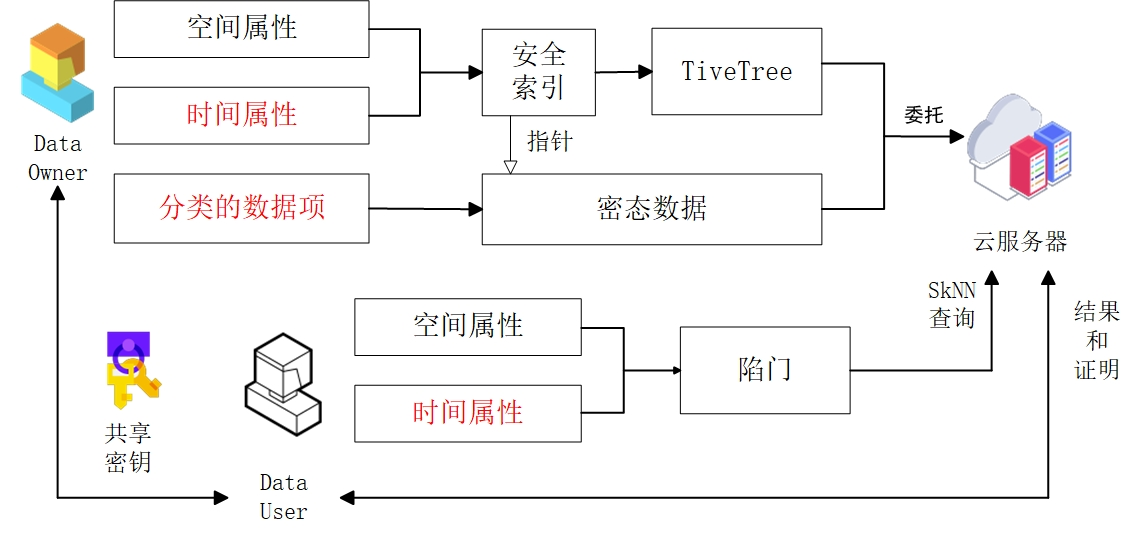
\includegraphics[width=0.8\textwidth]{jpgs/F1.jpg} % 请将your_image_file_name.png替换为实际图片文件名
    \caption{TiveQP系统模型}
    \label{fig:tiveqp_model}
\end{figure}
	
	\textbf{\bfseries\siyuan{数据拥有者}(Data Owner) }: 数据拥有者拥有一个包含 \(n\) 个数据项 \(\{L_1, L_2, \ldots, L_n\}\) 的数据集 \(D\)。每个数据项 \(L_i\) 有两个空间属性(位置类型和坐标)和一个时间属性(允许访问的时间段)。数据拥有者使用CPA安全加密算法加密每个数据项,并使用密钥和唯一随机数 \(r\) 为每个数据项构建一个安全索引 \(B\)。这些索引被分类并组织成一个包含自底向上验证信息的TiveTreeTR。然后,数据拥有者将TiveTree和加密的数据项外包给CS,并与经过身份验证的数据用户共享密钥。\par
	
	\textbf{\bfseries\siyuan{数据用户} (Combiner) }: 数据用户是期望获得时限请求的返回结果的用户,通过向云端发送位置和时限等信息进行最邻近(kNN)查询,并根据云端返回结果选择最佳的出行计划。数据用户使用查询位置的空间属性和时间属性构建一个陷门。这个陷门被发送给CS。数据用户收到CS的搜索结果后,使用共享密钥和随机数验证结果的正确性和完整性,然后解密数据项。\par
	
	\textbf{\bfseries\siyuan{云服务器} (Notary) }:云服务器存储TiveTree和加密的数据项,为数据用户处理最邻近(kNN)查询,并生成结果验证的证明。它将查询结果和证明返回给数据用户。\par
	
\subsubsection{补充定义}

\begin{enumerate}
    \item \textbf{\bfseries\siyuan{数据模型:}}数据集 D 由五个属性的记录组成:id(身份)、typ(位置类型)、lat(纬度)、lon(经度)和 per(允许访问时间)。数据集被安全地索引并存储在云上。
    \item \textbf{\bfseries\siyuan{索引树模型:}}索引树 TR 是一个包含叶子节点和非叶子节点的二叉树。叶子节点包含安全索引和验证信息,非叶子节点在树中聚合这些信息。该树分两个阶段构建,以确保数据的完整性和安全索引。
    \item \textbf{\bfseries\siyuan{查询模型:}}查询 Q 指定位置类型、坐标、访问时间和结果数量。系统支持对加密数据的安全查询,使用户能够验证结果的正确性和完整性。
    \item \textbf{\bfseries\siyuan{可验证的多维查询:}}该方案包括设置、索引、陷门生成、查询和结果验证的算法。它确保数据保密性、查询隐私性和结果可验证性,支持高效和安全的数据检索。其包含五个多项式时间算法。
\end{enumerate}

\subsubsection{威胁模型}

	隐私和安全威胁主要来自于外部和内部的攻击者。在系统外部,攻击者可以对系统内各个实体之间传递的消息进行窃听、重放、篡改等,尝试获取用户的身份隐私和位置隐私,或攻击系统的可用性从而导致系统瘫痪。

	威胁模型针对比以前的工作更强大的对手。除了对数据项、索引和查询感到好奇外,对手还可以篡改查询结果或访问数据集的部分内容。如果 CS 被对手或恶意员工攻破,这种攻击可能会发生。为了应对这些威胁,系统采用自适应选择关键词攻击下的不可区分性(IND-CKA)模型。该模型确保系统在对手可以基于先前知识选择关键词的自适应攻击下保持安全。

\subsubsection{设计目标}

安全性:为了防御半诚实体的攻击,我们利用安全索引和陷门来保护隐私。
\begin{itemize}
    \item 数据隐私:对手无法从安全索引和加密数据项中学到任何有用的信息。
    \item 查询隐私:对手无法从陷门中推断出任何有用的位置信息。
    \item 结果隐私:数据用户无法知道未匹配的数据项的任何信息,除了它们不匹配的事实。
\end{itemize}
结果可验证性:为了防御恶意云服务器的攻击,我们设计了一种隐私保护且高效的方法,允许数据用户验证查询结果 $R$。需满足两个要求:
\begin{itemize}
    \item 正确性:每个返回的数据项 $L$ 都没有被篡改,并且是真实存在于原始数据集 $L\in D$ 中的数据项。
    \item 完整性:所有返回的数据项都是SkNN查询的答案,所有其他数据项都不是。
\end{itemize}
系统允许数据用户验证查询结果的正确性和完整性。正确性确保每个返回的数据项未被篡改,并且确实是原始数据集的一部分。完整性确保所有返回的数据项都是查询的正确答案,并且没有遗漏正确的答案。


\subsection{实现原理}

在这部分,我们回顾用于构建 TiveQP 的四种基础技术,即空间编码、前缀编码、IBF(不可区分布隆过滤器)和 Merkle 树。

\subsubsection{空间编码}
空间编码是一种用于处理空间信息的关键技术,在数据管理和检索中发挥着重要作用。它通过一系列函数和操作,将地理位置信息转化为便于查询和处理的编码形式,以提升空间数据的处理效率。下面从函数和定义等方面详细介绍空间编码:
\begin{enumerate}
    \item 投影函数:投影函数是空间编码的首要步骤,它将地理位置映射到固定网格。设投影函数为\(project(lat, lon)\),其中\(lat\)代表位置的纬度,\(lon\)代表经度。该函数的作用是根据预设的网格划分规则,把经纬度坐标\((lat, lon)\)映射到一个具有唯一网格身份的固定网格\(g\)上。例如,在一个规则划分的网格系统中,对于某一特定位置\((lat_1, lon_1)\),经过\(project(lat_1, lon_1)\)的运算,能够确定其对应的网格为\(g_1\) 。从数学角度来看,这个映射关系可以简洁地表示为:\(g = project(lat, lon)\),这里的\(g\)就是目标网格,而\((lat, lon)\)则是输入的地理位置坐标。这种映射为后续的处理提供了基础的空间定位。
    \item 区域扩展函数:区域扩展函数是在投影得到单一网格的基础上,将其扩展为更宽的区域,以获取更多相关信息。定义扩展函数为\(expand(g)\),其中\(g\)是投影函数得到的输出,即单一网格。该函数的功能是根据特定的扩展规则,以\(g\)为中心,把它扩展为一组包含多个网格的区域\(G(lat, lon)\)。通常情况下,会以\(g\)为中心,向周围扩展8个相邻网格,从而形成一个包含9个网格的区域\(G\) 。用数学表达式表示为:\(G(lat, lon) = expand(g)\),其中\(G\)表示扩展后的区域,\(g\)是初始投影得到的网格。这种扩展操作能够涵盖更广泛的空间范围,为后续的查询提供更丰富的数据。
    \item 转换为最小前缀集函数**:最小前缀集函数负责将扩展后的区域转换为一种便于查询处理的集合形式。定义函数\(toMinPrefixSet(G)\),其中\(G\)是区域扩展函数的输出,即扩展后的区域\(G(lat, lon)\)。该函数会根据特定的编码规则,对\(G\)中的每个网格标识进行编码处理,生成一组具有特定前缀特征的集合,这个集合就是最小前缀集\(MS\) 。从数学角度表达为:\(MS = toMinPrefixSet(G)\),这里的\(MS\)表示最小前缀集,\(G\)表示扩展后的区域。最小前缀集的生成使得数据在后续的查询过程中能够更高效地进行匹配和筛选。
    \item 数据用户端的前缀族计算函数:在数据用户端,需要通过特定函数计算与最小前缀集匹配的前缀族。定义函数\(computePrefixFamily(gridId)\),其中\(gridId\)是数据用户根据自身当前位置提取的覆盖当前位置的网格标识。该函数会根据一定的算法,计算出与最小前缀集\(MS\)匹配的前缀族。例如,当数据用户确定当前位置对应的网格标识为\(gridId_1\)时,通过\(computePrefixFamily(gridId_1)\)函数的运算,就能得到相应的前缀族\(PF\) ,用于后续与\(MS\)进行匹配查询。数学表达式为:\(PF = computePrefixFamily(gridId)\),其中\(PF\)表示前缀族,\(gridId\)表示网格标识。通过计算前缀族,数据用户能够在最小前缀集中快速定位和筛选出符合自身需求的数据,提高查询效率 。 
\end{enumerate} 

\subsubsection{前缀编码}
在数据处理与信息检索领域,前缀编码是一项关键技术。以下从函数定义、操作步骤等方面详细阐述前缀编码:
\begin{enumerate}
    \item 前缀族定义函数:
给定一个\(w\)位的数字\(x\),其以二进制形式表示为\(x_1x_2\cdots x_w\) 。我们定义前缀族生成函数\(F(x)\),它用于生成数字\(x\)的前缀族。数学上,\(F(x)\)是一个包含\(w + 1\)个前缀的集合,具体表示为\(F(x)=\{x_1x_2\cdots x_w, x_1x_2\cdots x_{w - 1}*, \cdots, x_1* \cdots *, * * \cdots *\}\) 。这里的通配符“\(*\)”表示该位置可以取任意值。例如,对于一个4位二进制数\(x = 1011\),\(w = 4\),则\(F(1011)=\{1011, 101*, 10**, 1***, ****\}\) 。从形式化角度,对于任意\(w\)位二进制数\(x\),前缀族\(F(x)\)可通过如下方式生成:从完整的\(x\)的二进制表示开始,依次将最右边的一位替换为“\(*\)”,直到所有位都变为“\(*\)”为止 。
    \item 最小前缀集生成函数:
对于给定的范围\([A, B]\)(其中\(A\)和\(B\)均为二进制表示的数字),我们定义最小前缀集生成函数\(MF([A, B])\) 。该函数的作用是将范围\([A, B]\)转化为最小前缀集,使得这个最小前缀集的所有前缀的并集与\([A, B]\)等价。其生成过程较为复杂,通常基于二进制数的位运算和范围划分原理。例如,若\(A = 1000\),\(B = 1011\),通过特定算法处理后,可能得到\(MF([1000, 1011]) = \{100*, 101*\}\) 。数学上,设\(MF([A, B])=\{p_1, p_2, \cdots, p_n\}\),那么需要满足\(\bigcup_{i = 1}^{n} \text{range}(p_i)=[A, B]\) ,其中\(\text{range}(p_i)\)表示前缀\(p_i\)所涵盖的数字范围 。该函数确保生成的最小前缀集既能准确表示给定范围,又具有最小的规模,从而提高后续查询和匹配的效率 。
    \item 匹配判断函数:
为了判断数字\(x\)是否在范围\([A, B]\)内,我们定义匹配判断函数\(match(x, [A, B])\) 。此函数基于前缀族\(F(x)\)和最小前缀集\(MF([A, B])\)的交集进行判断。当且仅当\(F(x) \cap MF([A, B]) \neq \varnothing\)时,\(match(x, [A, B]) = \text{true}\),即\(x\)在范围\([A, B]\)内;反之,若\(F(x) \cap MF([A, B]) = \varnothing\),则\(match(x, [A, B]) = \text{false}\),意味着\(x\)不在范围\([A, B]\)内。例如,若\(x = 1010\),\([A, B] = [1000, 1011]\),由于\(F(1010)=\{1010, 101*, 10**, 1***, 1****, *****\}\),\(MF([1000, 1011]) = \{100*, 101*\}\),二者交集包含\(101*\),不为空集,所以\(match(1010, [1000, 1011]) = \text{true}\) 。从数学逻辑层面,匹配判断函数可形式化表示为:
\[match(x, [A, B]) = 
\begin{cases}
\text{true}, & \text{if } F(x) \cap MF([A, B]) \neq \varnothing \\
\text{false}, & \text{if } F(x) \cap MF([A, B]) = \varnothing
\end{cases}
\]
这种基于前缀编码的匹配判断方式,避免了对每个数字进行直接的范围比较,大大提高了范围查询的效率,在数据库索引、数据筛选等众多领域有着广泛的应用 。 
\end{enumerate} 

\subsubsection{IBF}

双布隆过滤器(IBF)是一种从布隆过滤器扩展而来的数据结构。具体来说,IBF是一个具有$N$对孪生单元的位数组$B$,其中每对孪生单元包含两个存储相反位的单元格。根据这种结构,我们可以同时存储和屏蔽关键字信息。我们将IBF总结为以下四种算法:
\begin{enumerate}
    \item 设置(Setup):$\text{Setup}(1^{n}, k) \to \{H_{key }, H\}$。此算法生成$k + 1$个带密钥的哈希函数$H_{key }=\{h_{i}:\{0,1\}^{*} \times \{0,1\}^{\eta} \to \{0,1\}^{*}\}$和一个哈希函数$H:\{0,1\}^{*} \to [0,1]$。这里,$H_{key }$可以通过使用带密钥的哈希消息认证码$HMAC$生成,即$h_{i}(\cdot)=HMAC(K_{i}, \cdot)$,$K_{i}$是随机生成的长度为$\eta$的秘密密钥。$H$可以使用随机预言机$\mathbb{H}:\{0,1\}^{*} \to \{0,1\}^{*}$生成,即$H = \mathbb{H}(\cdot)\%2$,用于确定选择哪个单元格。
    \item 初始化(Initi):$\text{Initi}(N, H_{k e y}, H, \gamma) \to B$。此算法生成$N$对孪生单元作为双布隆过滤器$B$。对于每对孪生单元,选定的单元格和未选定的单元格分别初始化为$0$和$1$,即
    \begin{align*} 
    &B[\iota][H(h_{k + 1}(\iota)\oplus \gamma)] = 0, \\ 
    &B[\iota][1 - H(h_{k + 1}(\iota)\oplus \gamma)] = 1, \iota \in[1, N], 
    \end{align*}
    其中$\gamma$是一个随机数,用于消除不同TBF之间的相关性。否则,$B_{i}$和$B_{j}$中第4对孪生单元的选定单元格会相同,这会降低随机性并增加数据暴露的风险。
    \item **插入(Insert)**:$\text{Insert}(B, w, H_{k e y}, H, \gamma) \to B$。对于集合$w$中的每个元素$w$,此算法首先将其哈希到$k$对孪生单元,即$B[h_{1}(w)], \cdots, B[h_{k}(w)]$,然后将这$k$对孪生单元中选定的单元格设置为$1$,未选定的单元格设置为$0$,即
    \begin{align*} 
    &B[h_{i}(w)][H(h_{k + 1}(h_{i}(w))\oplus \gamma)] = 1, \\ 
    &B[h_{i}(w)][1 - H(h_{k + 1}(h_{i}(w))\oplus \gamma)] = 0, i \in[1, k]. 
    \end{align*}
    \item 检查(Check):$\text{Check}(B, w, \gamma) \to 0/1$。为了测试元素$w'$是否存储在TBF $B$中,此算法计算并检查公式(4)。如果对于每个$i \in[1, k]$该式都成立,则$w'$在TBF $B$中。
    \[B[h_{i}(w')][H(h_{k + 1}(h_{i}(w'))\oplus \gamma)] \stackrel{?}{=} 1\]
    \item 正确性:如果对于所有安全参数$17$、$k \in \mathbb{Z}_{p}$、$N \in \mathbb{Z}_{p}$、$\gamma \in\{0,1\}^{*}$以及所有元素$w \in\{0,1\}^{*}$,都有$\{H_{k e y}, H\} \leftarrow \text{Setup}(1^{n}, k)$,$B \leftarrow \text{Initi}(N, H_{key }, H, \gamma)$,$B \leftarrow \text{Insert}(B, W, H_{k e y}, H, \gamma)$,并且当$w' \in W$时,$\text{Check}(B, w, \gamma)=1$,否则
    \[Pr[\text{Check}(B, w', \gamma)=0]=1 - negl_{1}(|W|, N, k),\]
    那么TBF是正确的。
\end{enumerate}
TBF的误报概率与传统布隆过滤器(BF)相同,计算为$negl_{1}(|W|, N, k)=(1-(1 - 1/N)^{|W|*k})^{k} \approx(1 - e^{-|W|*k/N})^{k}$。如果$|W| = 56$,$k = 10$,$N = 800$,则该概率为$(1 - e^{-56*10/800})^{10} \approx 0.1\%$ 。图1比较了TBF和BF在初始化和插入阶段的情况,其中TBF由10对孪生单元组成。我们观察到,TBF可以屏蔽插入位置和插入元素的数量,而BF则会完全暴露这些信息。

\subsubsection{Merkle 树}
Merkle树是一种在数据验证和完整性保护方面应用广泛的数据结构,常用于区块链、分布式系统等领域。以下从其定义、节点存在性验证以及批量验证等方面进行详细阐述:
\begin{enumerate}
    \item Merkle树的定义与结构:Merkle树是一棵完全二叉树,它依赖于一个哈希函数 \(H\) 和一个任意函数 \(a\)。对于树中的任意非叶节点 \(n_p\),设其两个子节点分别为 \(n_l\) 和 \(n_r\),则 \(n_p\) 的函数 \(a\) 值由如下公式确定:
    \[a(n_p) = H(a(n_l) \| a(n_r))\]
        其中,“\(\|\)”代表连接操作,即把两个子节点的函数值连接起来后,再经过哈希函数 \(H\) 计算。例如,若 \(n_l\) 的函数值 \(a(n_l)=x\),\(n_r\) 的函数值 \(a(n_r)=y\),那么 \(n_p\) 的函数值 \(a(n_p)=H(x\|y)\)。这种自底向上的计算方式,使得根节点的函数值能够综合反映整棵树的信息,可看作是整棵树数据的“摘要”。
\item 节点存在性验证:在Merkle树中,验证某个节点 \(n\) 的存在性可通过计算从 \(n\) 到根节点路径上的哈希值来实现。假设从节点 \(n\) 到根节点路径上的节点依次为 \(n_0 = n, n_1, \cdots, n_k\)(\(n_k\) 为根节点)。对于每个非根节点 \(n_i\)(\(0 \leq i < k\)),根据其在父节点中的位置计算哈希值:
    - 若 \(n_i\) 是其父节点 \(n_{i + 1}\) 的左子节点,则计算:
    \[H(a(n_i) \| a(\text{sibling}(n_i)))\]
    其中,\(\text{sibling}(n_i)\) 表示 \(n_i\) 的兄弟节点。例如,若 \(a(n_i)=m\),\(a(\text{sibling}(n_i)) = n\),则计算结果为 \(H(m\|n)\)。
    - 若 \(n_i\) 是其父节点 \(n_{i + 1}\) 的右子节点,则计算:
    \[H(a(\text{sibling}(n_i)) \| a(n_i))\]
    例如,当 \(a(\text{sibling}(n_i)) = p\),\(a(n_i)=q\) 时,计算结果为 \(H(p\|q)\)。
当完成从节点 \(n\) 到根节点路径上所有非根节点的哈希值计算后,若最终得到的根节点哈希值与预先存储的根节点哈希值相等,就表明节点 \(n\) 存在于Merkle树中。这是因为Merkle树的结构特点决定了每个节点的哈希值都基于其下一层子节点的哈希值计算,根节点哈希值是整棵树所有节点信息的综合体现。若计算得到的根节点哈希值与存储的根节点哈希值一致,就意味着从节点 \(n\) 到根节点路径上的所有节点信息都与Merkle树中的信息匹配,从而证明了节点 \(n\) 的存在性。
\item 批量验证:Merkle树还支持批量验证,这在处理大量数据验证时能显著提高效率。假设有一组节点 \(n_1', n_2', \cdots, n_s'\) 需要验证,我们可以同时计算这些节点到根节点路径上的哈希值。由于不同节点到根节点的路径可能存在部分重叠,在计算过程中可以共享这些重叠部分的中间计算结果。例如,节点 \(n_1'\) 和 \(n_2'\) 到根节点的路径在某一中间节点处重合,那么在计算这两个节点到根节点路径上的哈希值时,对于重合部分的中间计算结果无需重复计算,直接使用已有的结果即可。通过这种方式,能大幅减少计算量,提升验证效率。这种批量验证方式在实际应用中,如区块链中多个交易的验证、分布式系统中多个数据块的完整性验证等场景,发挥着重要作用,有助于提升系统的整体性能。 
\end{enumerate}

\subsection{系统方案}

我们在2.3.1节中介绍索引树,在2.3.2节展示如何计算陷门,在2.3.3节展示如何回答多维位置查询并生成证明,在2.3.4节讨论结果验证过程。TiveQP概述如图2.2所示,相关符号如表2.1。

\begin{figure}[H]
    \centering
    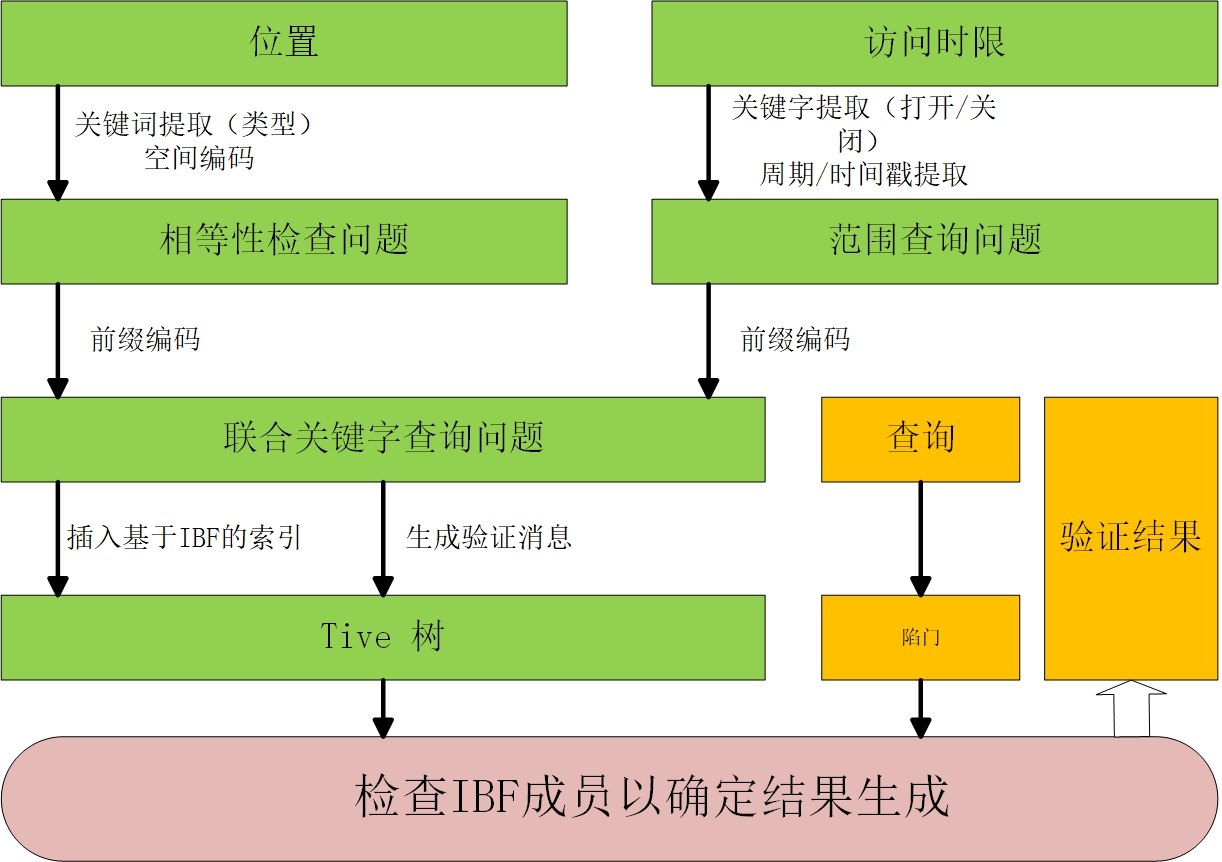
\includegraphics[width=0.8\textwidth]{jpgs/F2.jpg}
    \caption{TiveQP框架概述}
    \label{fig:tiveqp_framework}
\end{figure}

\begin{table}[h]
    \centering
    \begin{tabular}{ll}
        \toprule
        符号 & 定义 \\
        \midrule
        \(L\), \(D\), \(E\) & 数据项, 数据集, 加密数据项 \\
        \(B\), \(r\) & IBF, 随机数 \\
        \(k\), \(TR\) & 查询项个数, TiveTree \\
        \(di\), \(id\), \(typ\) & 数据项, 身份, 位置类型 \\
        \(lat\), \(lon\), \(per\) & 纬度, 经度, 访问时间段 \\
        \(g\), \(G(.)\), \(G\) & 网格, 网格函数, 网格集 \\
        \(MS\), \(F(.)\), \(PF\) & 最小前缀集, 前缀函数, 前缀族 \\
        \(w\), \(\{X_1, X_2, \cdots, X_2\}\), \(pr\) & 字段长度, 前缀码, 前缀 \\
        \(N\), \(m\) & 位数组长度, hash函数个数 \\
        \(\{h_1, h_2, \cdots, h_m\}\) & 伪随机hash函数 \\
        \(SK\) & 密钥 \\
        \(T\), \(T_1\) & 陷门, 类型陷门 \\
        \(T_2\), \(T_3\) & 位置陷门, 时间陷门 \\
        \(v\), \(root\) & 节点, 根节点 \\
        \(result\_num\), \(R\) & 结果集元素数, 结果集合 \\
        \(\epsilon\) & 密态数据项 \\
        \(z\) & 陷门行数 \\
        \(\pi\) & 证明集合 \\
        \(A\) & 对手 \\
        \bottomrule
    \end{tabular}
    \caption{TiveQP中的关键符号}
\end{table}


\subsubsection{构建索引}
我们假设服务区域被均匀地划分为一组网格 $G = \{g_1, g_2, \cdots\}$。考虑从“00:00”到“24:00”的时间段,并将每半小时编码为一个单位,从而将时间段变为 $[0, 47]$。

假设数据拥有者和数据用户共享 $m + 1$ 个秘密密钥 $SK = \{sk_1, sk_2, \cdots, sk_{m + 1}\}$ 和一个随机数 $r$。构建 $m$ 个伪随机哈希函数 $h_1, h_1, \cdots, h_m$,定义为 $h_i(.) = HMAC(.) \% N$ $(1 \leq i \leq m)$。另一个伪随机哈希函数定义为 $h_{m + 1}(.) = HMAC_{m + 1}(.)$。哈希函数定义为 $H(.) = SHA256(.) \% 2$。检查 $B_{kw}$ 用于检查关键字 $kw$ 是否存在于IBF $B$ 中,这里关键字是陷门中的一个元素,例如 $T = \{110, 11 *, 1 * *\}$ 有三个关键字。$QueLoc((B, kw))$ 通过查询IBF $B$ 中的关键字 $kw$ 输出一组位置值。

数据拥有者有一个位置数据集 $D = \{L_1, L_2, \cdots, L_n\}$,每个数据项 $L_i$ 是一个位置,具有身份、位置类型、纬度、经度和开放时间,如图2.3所示。例如,“银行”被转换为类型“100”,然后是最小前缀集。类似的操作应用于位置和开放时间。然后数据拥有者计算、存储和上传加密的数据项 $E$ 和TiveTree $TR$。首先,数据拥有者将每个 $L_i$ 加密为密文 $Enc(sk, L_i)$。其次,数据拥有者为每个 $L_i$ 计算安全索引如下:
\begin{enumerate}
    \item 提取 $typi$, $lat$, $lon$, $peri$。
    \item 给定两个坐标,定位到网格集 $G(i) = G(lat_i, lon_i)$,例如,一个汉堡店位于网格 $g_4$,其服务区域覆盖 $G = \{g_0, g_1, \cdots, g_8\}$。
    \item 生成随机数 $r$,通过设置 $B_{i}[h_o(pr)][H(h_{m + 1}(h_o(pr)) \oplus r)] = 1$ 和 $B_{i}[h_o(pr)][1 - H(h_{m + 1}(h_o(pr)) \oplus r)] = 0$,将 $G(i)$ 的最小前缀集中的每个前缀 $pr$ 插入到 $IBF\ B$ 中 $(1 \leq o \leq m)$。
    \item 将 $peri$ 编码为最小前缀集 $MS_i$,并将每个前缀插入 $B_i$,例如,“08:00 - 12:00”被编码为 $\{010***\}$。
\end{enumerate}

接下来,数据拥有者构建TiveTree $TR$ 如下:
\begin{enumerate}
    \item 根据类型和坐标对索引进行分类和排序;对于每种类型,构建一个从底部到顶部的子树,相应的索引作为叶节点,如2.4所示。
    \item 在每个子树中,对于叶节点 $v$ 上的每个数据项 $d_i$,计算位置补集(LCS)和时间补集(TCS)。
        \begin{itemize}
            \item LCS是覆盖 $d_i$ 位置之外区域的网格标识集。例如,总共有15个网格,当前数据项位于网格8,则其LCS为 $[1, 7][9, 15]$,其最小前缀集为 $\{0001, 001*, 01**,\ 1001, 101*, 11 **\}$。如果查询的位置落在节点的补充区域内,我们可以证明查询不匹配节点的IBF。
            \item TCS是数据项 $d_i$ 的闭馆时间。例如,开放时间为“08:00 - 12:00”,则其TCS为 $[0000, 0800] \cup [1200, 2400]$,转换为 $[0, 15] \cup [24, 47]$,其最小前缀集为 $\{0 *****, 11 *****, 10 * 1 *\}$。
        \end{itemize}
        对于LCS中的每个关键字 $w_j$,计算 $bits_{vj} = QueLoc(B_v, w_j)$ 和 $S_{vj} = HMAC_{sk0}(bits_{vj})$。定义 $bits_v$ 和 $S_v$ 为包含所有计算出的 $\{bits_{vj}\}$ 和 $\{S_{vj}\}$ 的两个集合。对于TCS,类似地计算 $bits_v$ 和 $S_v$。$\{bits, S\}$ 是完整性的证明。随后计算哈希值 $HV_v = hash(E_v)$ 作为正确性的证明。
    \item 在每个非叶节点 $v$(除了子树根节点)中,合并两个子节点的补集,构建新的LCS(TCS)以计算 $bits_v$ 和 $S_v$;计算 $B_v = B_{left} + B_{right}$ 和 $HV_v = hash(HV_{left} + HV_{right})$。
    \item 对于所有子树根节点 $v$ 及其父节点,计算 $B_v = B_{le} + B_{ri}$ 和 $HV_v = hash(HV_{le} + HV_{ri})$,将类型插入 $B_i$,插入类型补集(YCS)到 $B_v$ 并计算 $\{bits_v, S_v\}$。例如,如果有63种位置类型,$typ_v = 20$,YCS是编码的“$[1 - 19]\land[21 - 63]$”,即
        \[\{000001, 00001 *, 0001 * *, 001 * * *, 0100 * *, 0101, 01011 *, 011 * * *, 1 * * * * *\}\]
最终,数据拥有者将 $(E, TR, r)$ 外包给云服务器,并与数据用户共享根哈希值 $HV_{root}$。
\end{enumerate}

\begin{figure}[H]
    \centering
    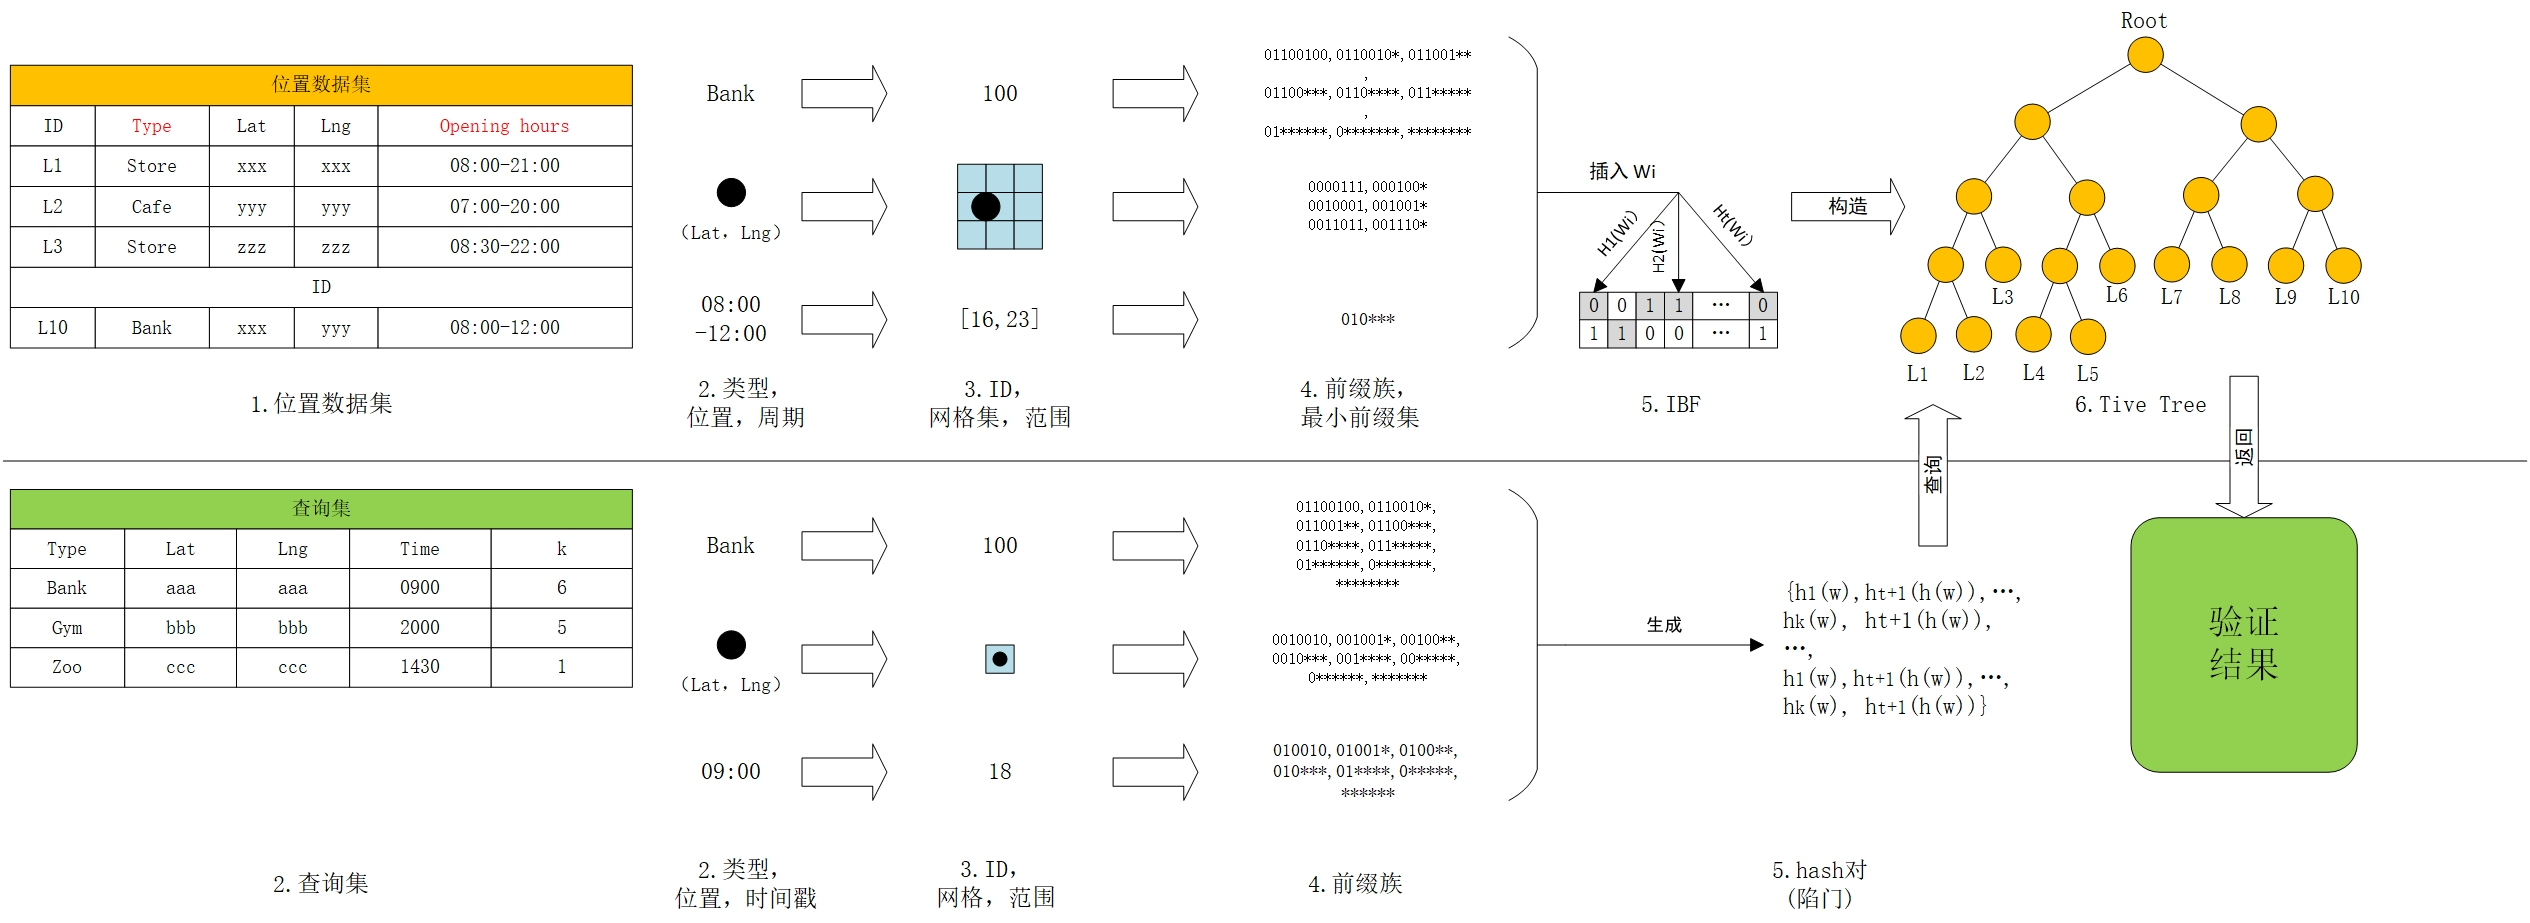
\includegraphics[width=0.8\textwidth]{jpgs/F3.jpg}
    \caption{TiveTree索引和查询处理}
    \label{fig:tivetree_index_query}
\end{figure}

\subsubsection{陷门计算}
一个数据用户有一个位置查询 $Q$,并计算一个陷门 $T = T_1 \cup T_2 \cup T_3$。这里,这三个集合是针对类型、坐标和时间准备的。
\begin{enumerate}
    \item 提取 $Q$ 的 $(typ, lat, lon, time)$,计算三个前缀族 $PF_1$、$PF_2$ 和 $PF_3$ ,用于 $typ$、$g(lat, lon)$ 和时间。例如,“09:00”编码为 $\{010010, 01001, 0100, 010, 01***, 0*****, ******\}$。
    \item 将 $(h_o(pr), H(h_{m + 1}(h_o(pr))))$ $(1\leq o\leq m, pr\in PF_1)$ 插入 $T_1$,将 $(h_o(pr), H(h_{m + 1}(h_o(pr))))$ $(1 \leq o \leq m, pr\in PF_2)$ 插入 $T_2$,将 $(h_o(pr), H(h_{m + 1}(h_o(pr))))$ $(1 \leq o \leq m, pr\in PF_3)$ 插入 $T_3$。
    \item 将 $T$ 发送给CS并等待查询结果和证明。
\end{enumerate}

\subsubsection{查询处理}
我们通过查找TiveTree中节点的IBF中的代码来回答查询。对于每个节点 $v$,我们通过将陷门中的每个元素映射到 $v$ 的IBF上来检查查询是否与 $v$ 中的前缀有共同元素。在查询过程中,CS还搜索三种类型的证据节点的证明。其思想是定位陷门中的一个前缀,该前缀可以查询匹配 $bits_v$ 中的字符串,即前缀与索引的补集(s)匹配。在深入研究搜索细节之前,我们介绍三种类型的证据节点。
\begin{enumerate}[label=\textbullet]
    \item 匹配叶节点(MLN):正确回答位置查询的叶节点。所有潜在的查询结果都存储在这些节点中。
    \item 不匹配节点(UMN):不匹配的非叶节点和不满足查询条件的叶节点。搜索在这些节点上停止。
    \item 不必要节点(UNN):在我们获得 $k$ 个匹配数据项时不需要搜索的节点。
\end{enumerate}
这三种证据节点被定义为对节点进行分类,并在搜索过程中帮助CS生成验证证明。它们的区别在于它们如何匹配搜索条件。CS从上到下搜索 $TR$,具体如下:
\begin{enumerate}
    \item 将当前搜索节点 $v$ 设置为根节点 $TR.root$,并设置 $result\_num = 0$。
    \item 在搜索进入子树之前,检查 $Check(B_v, T_1)$。
        \begin{enumerate}[label=(\arabic*)]
            \item 如果 $Check(B_v, T_1) = 1$ 并且 $v$ 是左节点,则将 $v$ 的右子节点临时设置为UNN,并沿着 $v$ 的左子树和右子树搜索 $T$;如果 $Check(B_v, T_1) = 1$ 并且 $v$ 是右节点,则移除之前设置的UNN标记并搜索 $v$ 的子树。
            \item 如果 $Check(B_v, T_1) = 0$,即在 $|T_1| = z * m$ 对哈希值 $\{(T_{ij}^{1}, T_{ij}^{2})\}$ 中,对于所有 $i$ 和一个 $j$,$1 \leq i \leq z$,$1 \leq j \leq m$,$B_v[T_{ij}^{1}][H(T_{ij}^{2} \oplus r)] = 0$,则标记 $v$ 为UMN并停止搜索。
        \end{enumerate}
        对于UMN,我们生成证明如下:
        \begin{enumerate}[label=(\arabic*)]
            \item 定位满足 $QueLoc (B, T) \in bits$ 的第一个前缀 $w \in T$。通过这种方式,我们获得一个证明,即通过证明 $typ$ 落在类型补集中,证明 $Q$ 不匹配 $D$。
            \item 将 $\{w_i, bits_{vi}, S_{vj}, HV_{v}\}$ 插入 $\pi$。
        \end{enumerate}
    \item 上述搜索递归地应用于子树,直到子根节点,最后一次检查 $T_1$ 以决定是否在子树中搜索 $T_1$ 和 $T_2$。
    \item 在每个子树中,对于节点 $v$,检查 $Check(B_v, T_2)$ 和 $Check(B_v, T_3)$。有两种情况:
        \begin{enumerate}[label=(\arabic*)]
            \item 如果两个查询都成功:$v$ 不是叶节点,则设置/移除UNN并继续类似地搜索子树;$v$ 是叶节点,则将 $v$ 标记为MLN,将 $\{HV_v\}$ 插入 $\pi$,将 $\{E_v\}$ 插入结果集 $R$ 并将 $result\_num$ 加1。如果找到 $k$ 个数据项,则停止递归并返回将所有UNN的HV插入到 $\pi$ 中。
            \item 如果存在一个不成功的查询,则将 $v$ 标记为UMN并停止搜索,在另一个陷阱集中搜索 $w_i$,并更新 $\pi$。
        \end{enumerate}
    \item 返回 $(R, \pi)$。
\end{enumerate}

\subsubsection{结果验证}
使用返回的证明 $\pi$,数据用户使用 $\pi$ 来验证结果集 $R$ 的正确性和完整性。
\begin{enumerate}[label=\textbullet]
    \item 验证正确性:数据用户需要验证 $R$ 是否正确以及CS是否创建了 $R$ 本身。首先,数据用户解密 $R$ 中的 $\epsilon$ 并检查她/他的查询是否与明文中的数据项匹配。其次,数据用户根据Merkle树从底部向上使用证据节点的哈希值HV重新计算根哈希值 $hash(root)$ 的值。如果 $hash(root)$ 等于数据所有者的哈希值 $hash(root)$,则数据用户确信 $R$ 是真实的,并且证据节点是TiveTree的真实节点。
    \item 验证完整性:在查询处理中,陷阱门 $T$ 从根向叶处理。查询处理过程直到陷门与叶节点匹配或者陷门不匹配TiveTree索引为止。每个匹配的数据项都有一个搜索路径,我们标记证据节点。因此,使用UMNs、MLNs和UNNs,数据用户可以为每个路径从下到上重现查询过程。
\end{enumerate}

\begin{figure}[H]
    \centering
    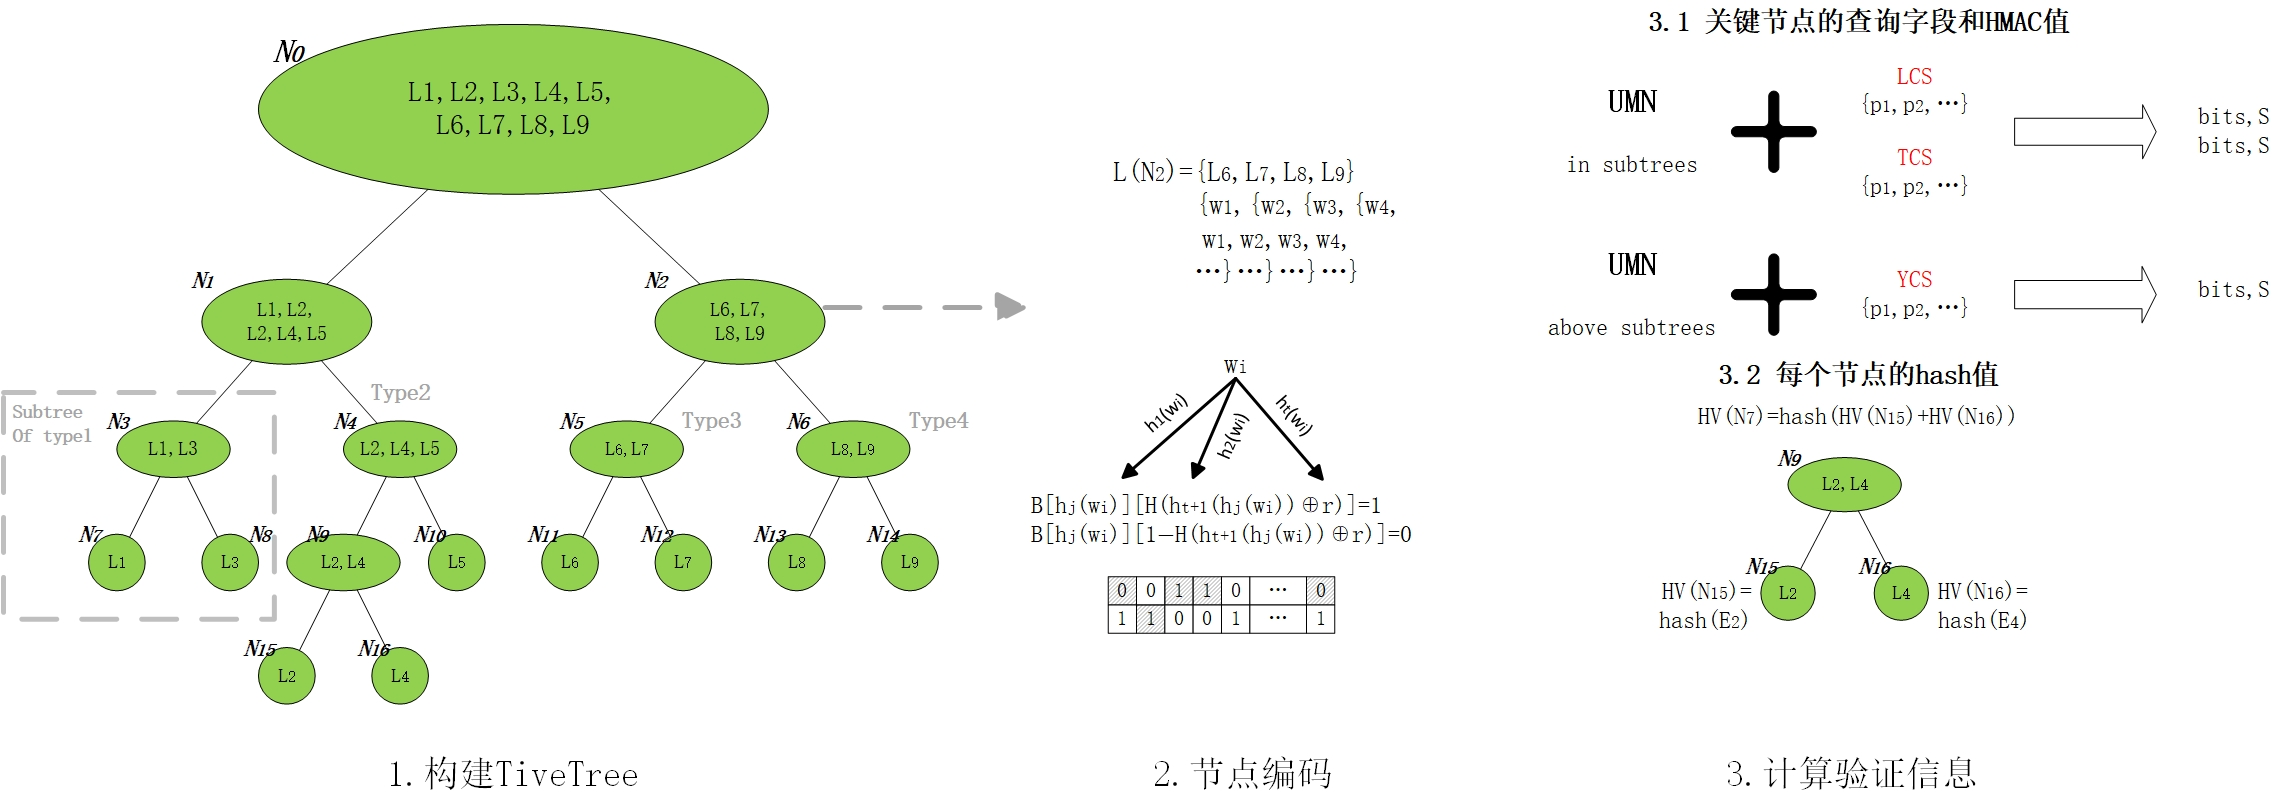
\includegraphics[width=0.8\textwidth]{jpgs/F4.jpg}
    \caption{对UMNs、MLNs和UNNs的验证结果树}
    \label{fig:verification_result_tree}
\end{figure}

如图2.5所示,我们使用Path 1和Path 2作为两个示例。假设具有 \(k = 2\) 的查询匹配 \(L_4\) 和 \(L_6\)。\(N_1\) 匹配具有 \(L_4\) 的查询,其左子节点标记为UMN,表示不匹配查询。搜索在 \(N_1\) 的右子树中继续,直到节点N16匹配查询,该节点标记为MLN。最后,Path 1为 \(N_0 \to N_1 \to N_4 \to N_9 \to N_{16}\)。在Path 2上,我们注意到有两个UNN,\(N_{12}\) 和 \(N_6\)。它们被标记是因为当搜索到达 \(N_{11}\) 时我们获得 \(k = 2\) 个数据项。因此,我们不需要搜索 \(N_{12}\) 或 \(N_6\)。

对于每个搜索路径,UMNs、MLNs和UNNs的并集必须忠实地重现搜索。如果CS故意忽略了一些节点,结果集将不完整。

\newpage

\section{安全与隐私性证明}

我们证明了该算法在自适应IND - CKA模型下是安全的。我们分别使用HMAC和SHA256来实现哈希函数\(h_{1}, h_{2}, \cdots, h_{m + 1}\)和\(H\)。当且仅当函数输出和真正随机函数输出不能被概率多项式时间(Probabilistic Polynomial Time,PPT)对手区分时,一个函数是伪随机函数\([12],[6]\)。在模拟中选择未来的查询之前,PPT对手\(A\)可以查看其过去的查询和相应的陷阱门、结果和证明。

为了证明TiveQP在自适应IND - CKA模型下是安全的,我们首先构建了一个可以模拟未来查询的PPT模拟器\(s\)。接下来,我们证明了与\(s\)相互作用的\(A\)面临着以不可忽略的概率区分真实安全指标和\(s\)中的指标的挑战。从形式上看,如果PPT攻击者\(A\)不能区分伪随机函数生成的真实索引和真正随机函数生成的模拟索引,那么查询处理方案是安全的,并且具有不可忽略的概率:
\[|Pr[Real_{A, C}(1^{\lambda}) = 1] - Pr[Ideal_{A, s}(1^{\lambda}) = 1]| \leq negl(\lambda)\]
其中,\(negl(\lambda)\)是一个可忽略的函数。我们定义两个泄漏函数如下:
\begin{itemize}
    \item \(L_{1}(D) = (n, N, TR,|E|)\):给定位置数据集\(D\),\(L_{1}\)输出数据集大小\(n\)、IBF位长度\(N\)、TiveTree \(TR\)和密文位长度\(|E|\)。
    \item \(L_{2}(D, Q) = (\alpha(Q), \beta(Q), \gamma(Q))\):给定一个位置数据集\(D\)和一个位置查询\(Q\),\(L_{2}\)输出由查询\(\alpha(Q)\)、搜索模式\(\beta(Q)\)和路径模式\(\gamma(Q)\)返回的数据项\(id\)。
\end{itemize}

定理1(安全性):在随机oracle模型中,针对自适应\(A\),TiveQP是\(IND - CKA(L_{1}, L_{2})\) - 安全的。

证明:我们首先构造\(s\)来模拟视图\(V^{*} = (TR^{*}, T^{*}, E^{*})\),基于\(L_{1}(TR, D)\)和\(L_{2}(TR, D, Q)\);接下来,我们证明\(A\)不能区分\(V^{*}\)和真正的对手观点\(A\)。
\begin{itemize}
    \item 为了模拟\(TR^{*}\),\(s\)首先构建一个结构相同的TiveTree。\(s\)从\(L_{1}\)获取\(N\),并为\(TR\)中的每个节点\(v\)建立IBF \(B_{v}\)。在\(B_{v}\)的第\(i\)个单元格中,\(s\)设\(B_{v}[i][0] = 1\),\(B_{v}[i][1] = 0\),反之亦然。双胞胎是通过抛硬币来决定的。接下来,\(s\)将\(B_{v}\)与随机选择的数字\(r\)关联起来。对于验证信息,\(s\)为每个叶节点随机选择一个网格,计算相应的LCS和TCS,并生成\(bits_{v}\)和\(S_{v}\)。\(s\)继续这个步骤,直到子树节点,并为每个节点计算YCS,直到根节点。最后,\(s\)将\(TR^{*}\)返回给\(A\)。\(TR^{*}\)中的每个IBF \(B_{v}\)与\(TR\)中的\(IBF B_{v}\)大小相同。它们的\('0's\)和\('1's\)是均匀分布的。因此,\(A\)不能区分模拟的\(TR^{*}\)和真实的\(TR\)。
    \item 为了模拟\(T^{*}\),\(s\)知道接收到的\(Q\)是否已经从\(C_{2}\)被处理。如果是,\(s\)将之前的陷阱门\(T\)返回给\(A\)。否则,\(s\)生成一个新的陷阱门\(T^{*}\),它是\(m\)对哈希的集合。给定来自\(L_{2}\)的访问模式,\(s\)知道哪些数据项与\(T\)匹配。对于MLF,\(s\)通过使用\(H\)选择\(e\)对哈希来生成输出,同时满足所选哈希对与MLF匹配。对于不匹配的叶节点,\(s\)通过使用随机oracle将\(T\)与叶节点不匹配来生成输出。哈希的\(e\)对是\(T^{*}\)。因为陷门是由随机哈希函数产生的,所以\(A\)不能区分\(T^{*}\)和真实的陷门。
    \item 为了模拟\(E^{*}\),\(s\)首先从\(L_{1}\)获取\(n\)和\(|E|\)。接下来,\(s\)用随机明文模拟密文集,已知的CPA安全加密算法Enc。\(s\)必须确保模拟密文的大小与真实密文的大小相同。
\end{itemize}
综上所述,模拟视图和真实视图是\(A\)无法区分的,因此,在随机oracle模型中,TiveQP是自适应的\(IND - CKA(L_{1}, L_{2})\)安全的,即实现了索引隐私和查询隐私。此外,CS不像\([18]\)那样将叶节点的IBF返回给数据用户,而只返回一个位串和一个HMAC。数据所有者只能验证查询的不匹配,不能在IBF上插入其他查询的陷门。因此,实现了结果隐私。


\newpage

\section{系统实现}

\subsection{系统部署}

根据实际情况添加相应部署内容。

\subsection{后端搭建}
可描述后端使用的编程语言、框架,数据库选型及配置等。

\subsection{前端搭建}
前端搭建涉及多种技术栈,以下是详细介绍:
\begin{itemize}
    \item \textbf{Vue3}:Vue 3 是构建前端界面的核心框架,带来了诸多显著提升。其采用 Proxy 实现响应式系统,相比 Vue 2 的 Object.defineProperty,性能大幅飞跃。Proxy 能劫持对象操作,精准追踪数据变化,减少不必要更新。组合式 API 是一大亮点,它让代码结构更清晰,便于维护与扩展。开发时可将逻辑关注点封装成独立函数,按需引入使用,避免了 Vue 2 选项式 API 代码碎片化问题,尤其在处理复杂逻辑时优势明显。同时,Vue 3 对 TypeScript 支持更佳,结合 \texttt{<script setup lang="ts">} 语法,能充分发挥静态类型检查优势,为组件的 props、emits、data 等定义明确类型,在开发阶段就发现潜在类型错误,提高代码可靠性。本作品中使用 Vue 3 搭建网页前端界面。
    \item \textbf{Vite}:Vite 作为项目构建工具,赋予了我们快速的开发体验。它基于原生 ES 模块,开发阶段无需打包,启动速度极快。当修改代码时,能实现即时热重载,几乎瞬间更新页面,极大提高了开发效率。Vite 拥有丰富的插件生态,例如 \texttt{@vitejs/plugin - vue} 专门处理 Vue 3 组件编译,可无缝集成 Vue 3 应用到项目中。在生产环境,Vite 使用 Rollup 打包,支持 Tree Shaking 功能,能自动移除未使用代码,减小打包文件体积,提升应用加载速度。本作品中使用 Vite 构建和开发网页前端项目。
    \item \textbf{Element Plus}:Element Plus 是基于 Vue 3 的 UI 组件库,为我们提供了丰富多样的可复用组件。其组件库涵盖按钮、输入框、表格、菜单等常见 UI 组件,具有统一设计风格和良好交互性,直接在项目中使用这些组件,无需从头编写样式和交互逻辑,大大提高了开发效率。而且,Element Plus 提供完善文档和示例,方便我们对组件进行定制和扩展,可通过修改组件属性、插槽等实现个性化需求,如自定义按钮样式、修改表格列配置等。此外,它还支持国际化,引入相应语言包就能轻松实现多语言切换,满足不同地区用户需求。本作品中部分组件使用了 Element Plus。
    \item \textbf{Vue Router}:Vue Router 是 Vue.js 官方的路由管理器,用于实现单页面应用(SPA)的路由功能。通过配置路由规则,可实现不同页面之间的导航和切换。在项目里,我们定义不同路由路径和对应组件,用户访问不同路径时,Vue Router 自动渲染相应组件。同时,它支持路由守卫,能在路由切换前进行验证和处理,比如检查用户是否登录,未登录则跳转到登录页面,提高应用安全性。另外,为提升应用性能,Vue Router 支持路由懒加载,将路由对应的组件进行懒加载,用户访问该路由时才加载相应组件,减少初始加载文件体积,加快应用启动速度。Vue Router 是本作品中用于实现单页面应用(SPA)路由功能的核心工具,为用户提供了流畅的页面导航体验。
    \item \textbf{TypeScript}:TypeScript 作为 JavaScript 的超集,为项目带来了静态类型检查的优势。在项目中,我们用它编写组件逻辑、接口定义和类型注解。静态类型检查能在开发阶段发现潜在类型错误,避免运行时出现类型相关问题,例如为函数参数和返回值定义明确类型,调用函数时若传入参数类型不符,TypeScript 会立即提示错误。而且,类型注解让代码更清晰易懂,其他开发者阅读代码时能快速了解变量和函数用途及类型,也有助于代码重构和维护,修改代码时能及时发现因类型不匹配导致的问题。此外,Vue 3 对 TypeScript 提供了良好支持,在 \texttt{tsconfig.json} 和 \texttt{tsconfig.app.json} 中配置编译选项,确保 TypeScript 代码能正确编译和运行。TypeScript 为本作品带来了静态类型检查,提升了代码的可靠性和可维护性。
\end{itemize}

\subsection{开发工具及环境配置}
本作品的开发过程使用了多种工具和技术,以确保系统的高效、可靠和可扩展性。这些技术和工具不仅提高了开发效率,也增强了系统的稳定性和安全性。开发过程中,我们使用的软件环境如下(假设此处后续会补充表格,这里仅占位说明):

开发工具及环境配置涵盖前端和后端两部分技术栈,前端已在前端搭建部分详细介绍,后端技术栈如下:
\begin{itemize}
    \item \textbf{Go 语言}:Go 语言是由 Google 开发的开源静态类型、编译型编程语言,它巧妙融合了传统编译型语言的高性能与脚本语言的高效开发特性。其具有显著优势:一是编译速度极快,运行时配备高效的垃圾回收机制,能有效降低内存开销,大幅提升程序整体性能;二是内置轻量级线程(goroutine)和通道(channel),极大简化了并发编程复杂度,让开发者可轻松编写高并发程序,充分发挥多核处理器性能;三是语法简洁易懂,减少了冗余代码,提高了代码的可读性与可维护性。在本作品里,Go 语言承担着编写系统核心逻辑的重任,涵盖数据加载、树的构建、陷门生成、查询以及结果验证等功能。
    \item \textbf{Go 标准库}:Go 标准库为 Go 语言开发者提供了涵盖文件操作、网络编程、加密解密、数据结构等多领域的丰富功能与工具。在本作品中,主要运用了多个标准库包,其中 \texttt{crypto} 包提供各类加密和哈希算法,像 \texttt{crypto/sha256} 可计算 SHA - 256 哈希值、\texttt{crypto/hmac} 能计算 HMAC 哈希值,以此确保数据的完整性和安全性;\texttt{math/big} 包可处理大整数,在密码学计算和索引计算中,能准确应对超出普通整数范围的数值;\texttt{bytes} 包提供字节切片的操作方法,便于对字节数据进行处理和转换;\texttt{rand} 包用于生成随机数,在加密和初始化过程中发挥了重要作用。
    \item \textbf{并发编程模型(goroutine 和 channel)}:Go 语言的并发编程模型以 goroutine 和 channel 为核心,为开发者提供了强大的并发编程能力,使得开发者能够轻松编写出高并发的程序。goroutine 是一种轻量级的线程,由 Go 运行时管理,相较于传统的线程,它的创建和销毁开销极小,并且可以在单个操作系统线程上运行多个 goroutine,从而充分利用多核处理器的性能。而 channel 则是一种用于在 goroutine 之间进行通信和同步的机制,它可以确保数据在不同的 goroutine 之间安全地传递,避免了共享内存带来的并发问题。
    在本作品中,充分利用了 Go 语言的并发编程特性,通过使用 goroutine 并行构建子树,显著提高了树的构建效率。具体来说,在构建树的过程中,将所有的 owner 数据分成多个小块,每个小块包含 1000 个元素。对于每个小块,启动一个独立的 goroutine 来构建子树。这样,多个子树可以同时构建,而不是按顺序依次构建,大大减少了总的构建时间。
    同时,为了确保并发操作的安全性和稳定性,本作品使用 channel 进行结果的传递和错误处理。定义了两个 channel:一个用于接收构建好的子树根节点,另一个用于接收构建过程中出现的错误。每个 goroutine 在完成子树构建后,将结果发送到对应的 channel 中。主 goroutine 通过监听这些 channel,收集所有子树的构建结果,并处理可能出现的错误。如果在构建过程中出现错误,主 goroutine 会立即停止后续的操作,并返回错误信息。
    \item \textbf{测试框架}:使用 Go 的 \texttt{testing} 包进行单元测试,编写了多个测试用例来验证各个模块的功能。通过单元测试,可以确保系统的稳定性和正确性,及时发现和修复潜在的问题。在本作品中,\texttt{main\_test.go} 和 \texttt{all\_test.go} 文件中包含了对数据加载、树构建、加密解密等功能的测试。
\end{itemize}

\newpage

\section{作品测试与分析}
\subsection{测试目的}
本系统的测试旨在验证各个组成部分的功能完整性和性能表现,确保整个系统的稳定运行和安全性。主要目标包括:
\begin{enumerate}
    \item \textbf{功能测试}:
        \begin{itemize}
            \item 索引构建功能:确保Index算法能准确地对数据所有者的位置数据集进行加密处理,构建出安全的TiveTree索引。验证每个数据项的空间和时间属性都被正确编码并插入到相应的IBF中,同时检查各类互补集(如LCS、TCS、YCS)的计算和插入是否准确无误。
            \item 陷门计算功能:确认Trapdoor算法能根据用户的查询条件,正确生成用于查询的陷门。验证陷门中的前缀编码和哈希值计算是否正确,确保其能准确反映用户的查询需求。
            \item 查询处理功能:验证Query算法能在TiveTree索引中高效准确地进行查询。检查查询过程中对各类节点(如MLN、UMN、UNN)的判断和处理是否正确,确保返回的查询结果集 \(R\) 和证明集 \(\pi\) 准确无误,且符合查询条件。
            \item 结果验证功能:通过Verify算法验证查询结果的正确性和完整性。确保数据用户能够利用证明集 \(\pi\),准确验证返回的结果集 \(R\) 未被篡改,且包含所有符合查询条件的数据项,同时验证查询过程的真实性和完整性。 
        \end{itemize}
    \item \textbf{计算开销测试}:
        \begin{itemize}
            \item 索引构建阶段:评估Index算法在构建TiveTree索引时的计算资源消耗,包括计算前缀编码、插入IBF、计算互补集、生成哈希值等操作所占用的CPU时间和内存资源。分析不同规模数据集(如不同数量的数据项 \(n\)、不同的位置类型 \(t\))和不同网格宽度 \(gw\) 对索引构建计算开销的影响。
            \item 陷门计算阶段:测量Trapdoor算法生成陷门时的计算开销,主要包括前缀编码和哈希值计算所消耗的资源,探究查询参数(如查询类型、位置、时间)对陷门计算开销的影响。
            \item 查询处理阶段:测试Query算法在查询过程中的计算资源消耗,重点关注遍历TiveTree索引、检查陷阱门与IBF的匹配、生成证明集等操作的计算开销。分析数据规模(数据项数量 \(n\)、位置类型 \(t\))、网格宽度 \(gw\) 以及查询参数 \(k\) 对查询处理计算开销的影响,验证查询时间复杂度是否符合理论预期 \(O(k \log (\frac{n}{t c}))\)。
            \item 结果验证阶段:评估Verify算法验证查询结果时的计算开销,包括解密数据项、重新计算根哈希值以及检查证明集等操作所消耗的资源。分析结果集大小、证明集内容以及数据规模对结果验证计算开销的影响。
        \end{itemize}
    \item \textbf{通信代价测试}:
        \begin{itemize}
            \item 数据上传阶段:测量数据所有者将加密数据项和TiveTree索引上传至云服务器时的数据传输量和传输时间,分析数据集规模(数据项数量 \(n\)、位置类型 \(t\))对上传通信代价的影响。
            \item 查询请求与响应阶段:评估数据用户向云服务器发送查询请求以及接收查询结果和证明集时的通信开销,包括查询请求消息大小、响应消息(结果集 \(R\) 和证明集 \(\pi\))大小以及传输时间。分析查询参数(如查询类型、位置、时间、查询数量 \(k\))对通信代价的影响,研究不同网络环境下的传输效率。
            \item 多节点交互阶段:若涉及多个数据用户或云服务器之间的交互(如在分布式场景下),测试节点之间的数据传输量和传输延迟,评估系统在复杂网络环境中的通信性能。
        \end{itemize}
\end{enumerate}

这些测试将帮助我们识别和解决潜在问题,优化系统性能,从而提供可靠、高效且安全的服务。

\subsection{测试环境}
数据集:我们使用来自美国和加拿大836个城市的Yelp商家和用户数据集\cite{文献1,文献2}。我们将所有的源代码、处理后的数据集以及一份说明文件上传到了\url{https://github.com/UbiPLab/TiveQP}。由于原始数据集过大(4.9GB),我们仅提供一个链接。

参数:我们将 \(n\) 的值从10,000变化到100,000,位置类型 \(t\) 从20变化到100,位置宽度 \(gw\) 从1变化到5公里,\(k\) 从1变化到50。根据FPR等式\cite{文献3,文献4},一个IBF的结果大小范围从24KB到120KB。(假设此处有详细参数设置表,需用tabular环境编写,示例如下)
\begin{table}[h]
    \centering
    \begin{tabular}{|c|c|c|c|}
        \hline
        参数 & 最小值 & 最大值 & 默认值\\
        \hline
        \(n\) & 10000 & 100000 & 20000\\
        \hline
        \(t\) & 20 & 100 & -\\
        \hline
        \(gw\) & 1(公里) & 5(公里) & -\\
        \hline
        \(k\) & 1 & 50 & -\\
        \hline
    \end{tabular}
    \caption{详细参数设置}
\end{table}
默认参数值 \(n\) 设置为20000,我们在回顾相关文献时发现,这是当前最先进的实验设置,且是一个相对较高的值。

基线方法:为了评估安全的多维度查询框架的查询性能,我们将TiveQP与六种基线方法进行比较:(1)PBtree\cite{文献5}支持对单维数据进行范围查询。(2)IBtree\cite{文献6}通过使用布隆过滤器(IBF)实现合取查询处理。(3)SecEQP\cite{文献7}基于基于投影的函数和布隆过滤器(IBF)对位置进行编码。(4)ServeDB\cite{文献8}支持多维度且可验证的范围查询。(5)R*-树\cite{文献9}是一种用于对空间信息进行索引的动态树结构。(6)无类型的TiveQP与TiveQP类似,但它的数据项中没有类型信息。

实验设置:我们在一台个人计算机服务器上进行了实验。该服务器运行的是Windows Server 2021 R2数据中心版操作系统,配备主频为3.7 GHz的英特尔(R)酷睿(TM)i7 - 8770K处理器以及32GB随机存取存储器(RAM)。我们使用HMAC - SHA256(哈希消息认证码 - 安全散列算法256)作为伪随机函数来实现布隆过滤器(IBF)的哈希函数。我们采用高级加密标准(AES)作为对称加密算法。由于在对数据项进行加密时,高级加密标准(AES)可同时应用于TiveQP和其他方案,因此在对比中,我们将重点放在索引上,并排除了加密结果。

\subsection{功能性测试}

\subsubsection{索引构建}
此处内容待补充(可描述索引构建的测试方法、测试用例、预期结果等,示例:采用[具体测试工具]对不同规模的数据集进行索引构建测试,预期在[时间范围]内完成构建,且构建的索引能准确反映数据特征等)

\subsubsection{检索测试}
此处内容待补充(可介绍检索测试的场景、查询条件设置、评估检索准确性和效率的指标等,示例:设置不同的查询条件,如空间范围查询、时间范围查询等,通过对比实际返回结果与预期结果来评估检索准确性,记录查询响应时间来衡量检索效率)

\subsubsection{正确性验证}
数据用户需要验证 $R$ 是否正确,以及云服务器(CS)是否伪造了 $R$。首先,数据用户解密 $R$ 中的加密数据项 $\varepsilon$,并检查其查询是否与明文数据项匹配。其次,数据用户根据 Merkle 树\cite{30},利用证明 $\pi$ 中证据节点的哈希值 $\{HV\}$,自底向上重新计算根哈希值 $\text{hash}'(\text{root})$。如果 $\text{hash}'(\text{root})$ 与数据所有者的根哈希值 $\text{hash}(\text{root})$ 相等,数据用户就可以确信 $R$ 是真实的,并且证据节点是 TiveTree 的真实节点。

\subsubsection{完备性验证}
在查询处理过程中,陷门 $T$ 从根节点向叶节点进行处理。直到陷门与叶节点匹配,或者陷门与 TiveTree 索引不匹配时,查询过程才会终止。每个匹配的数据项都有一条搜索路径,我们会标记该路径上的证据节点。因此,利用未匹配节点(UMNs)、匹配叶节点(MLNs)和不必要节点(UNNs),数据用户可以自底向上重现每条路径的查询过程。

\subsection{计算开销测试}
\subsubsection{构建耗时}
随着 \(n\) 从20增长到100K(千)且位置宽度 \(gw\) 从1千米增加到5千米,TiveQP的构建时间分别从3.58分钟增长到19分钟,以及从3.58分钟减少到1.54分钟。在图5.1(a)和图5.1(b)中:

\begin{figure}[h]
    \centering
    \begin{subcaptionbox}{Construction time varying \(n\)}
        {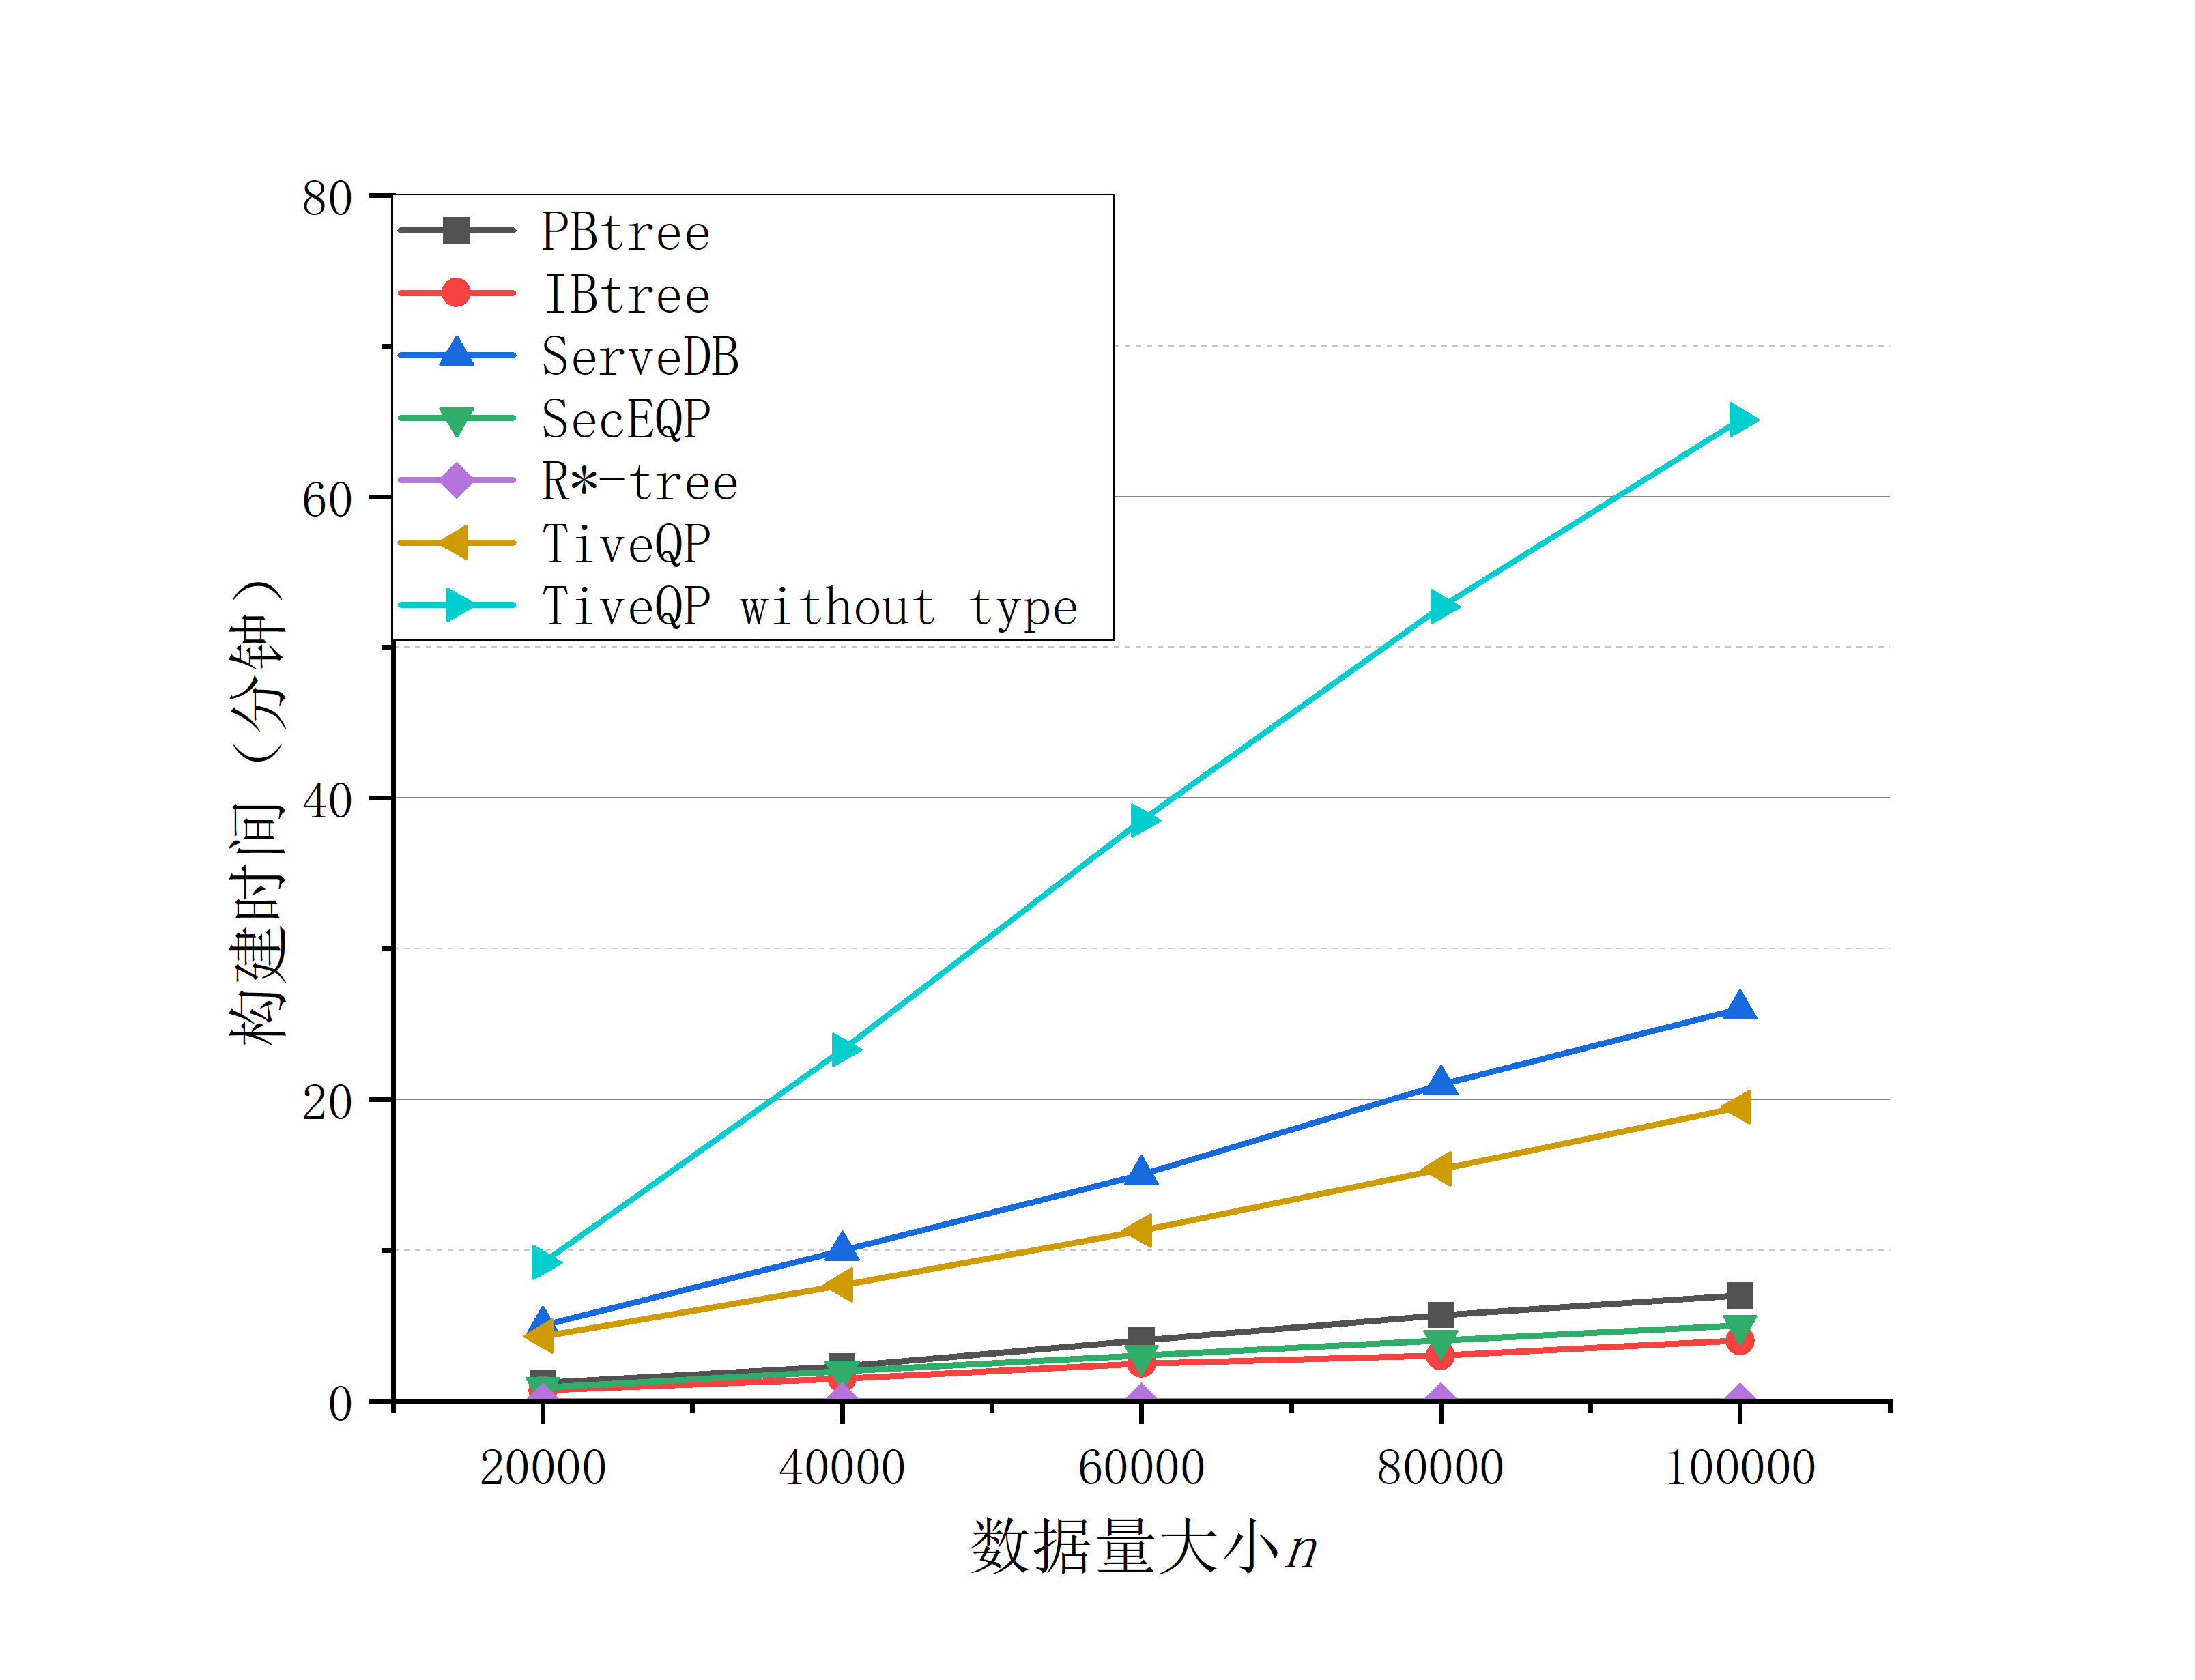
\includegraphics[width=0.45\textwidth]{jpgs/6-a.png}}
    \end{subcaptionbox}
    \hfill
    \begin{subcaptionbox}{Construction time varying \(gw\)}
        {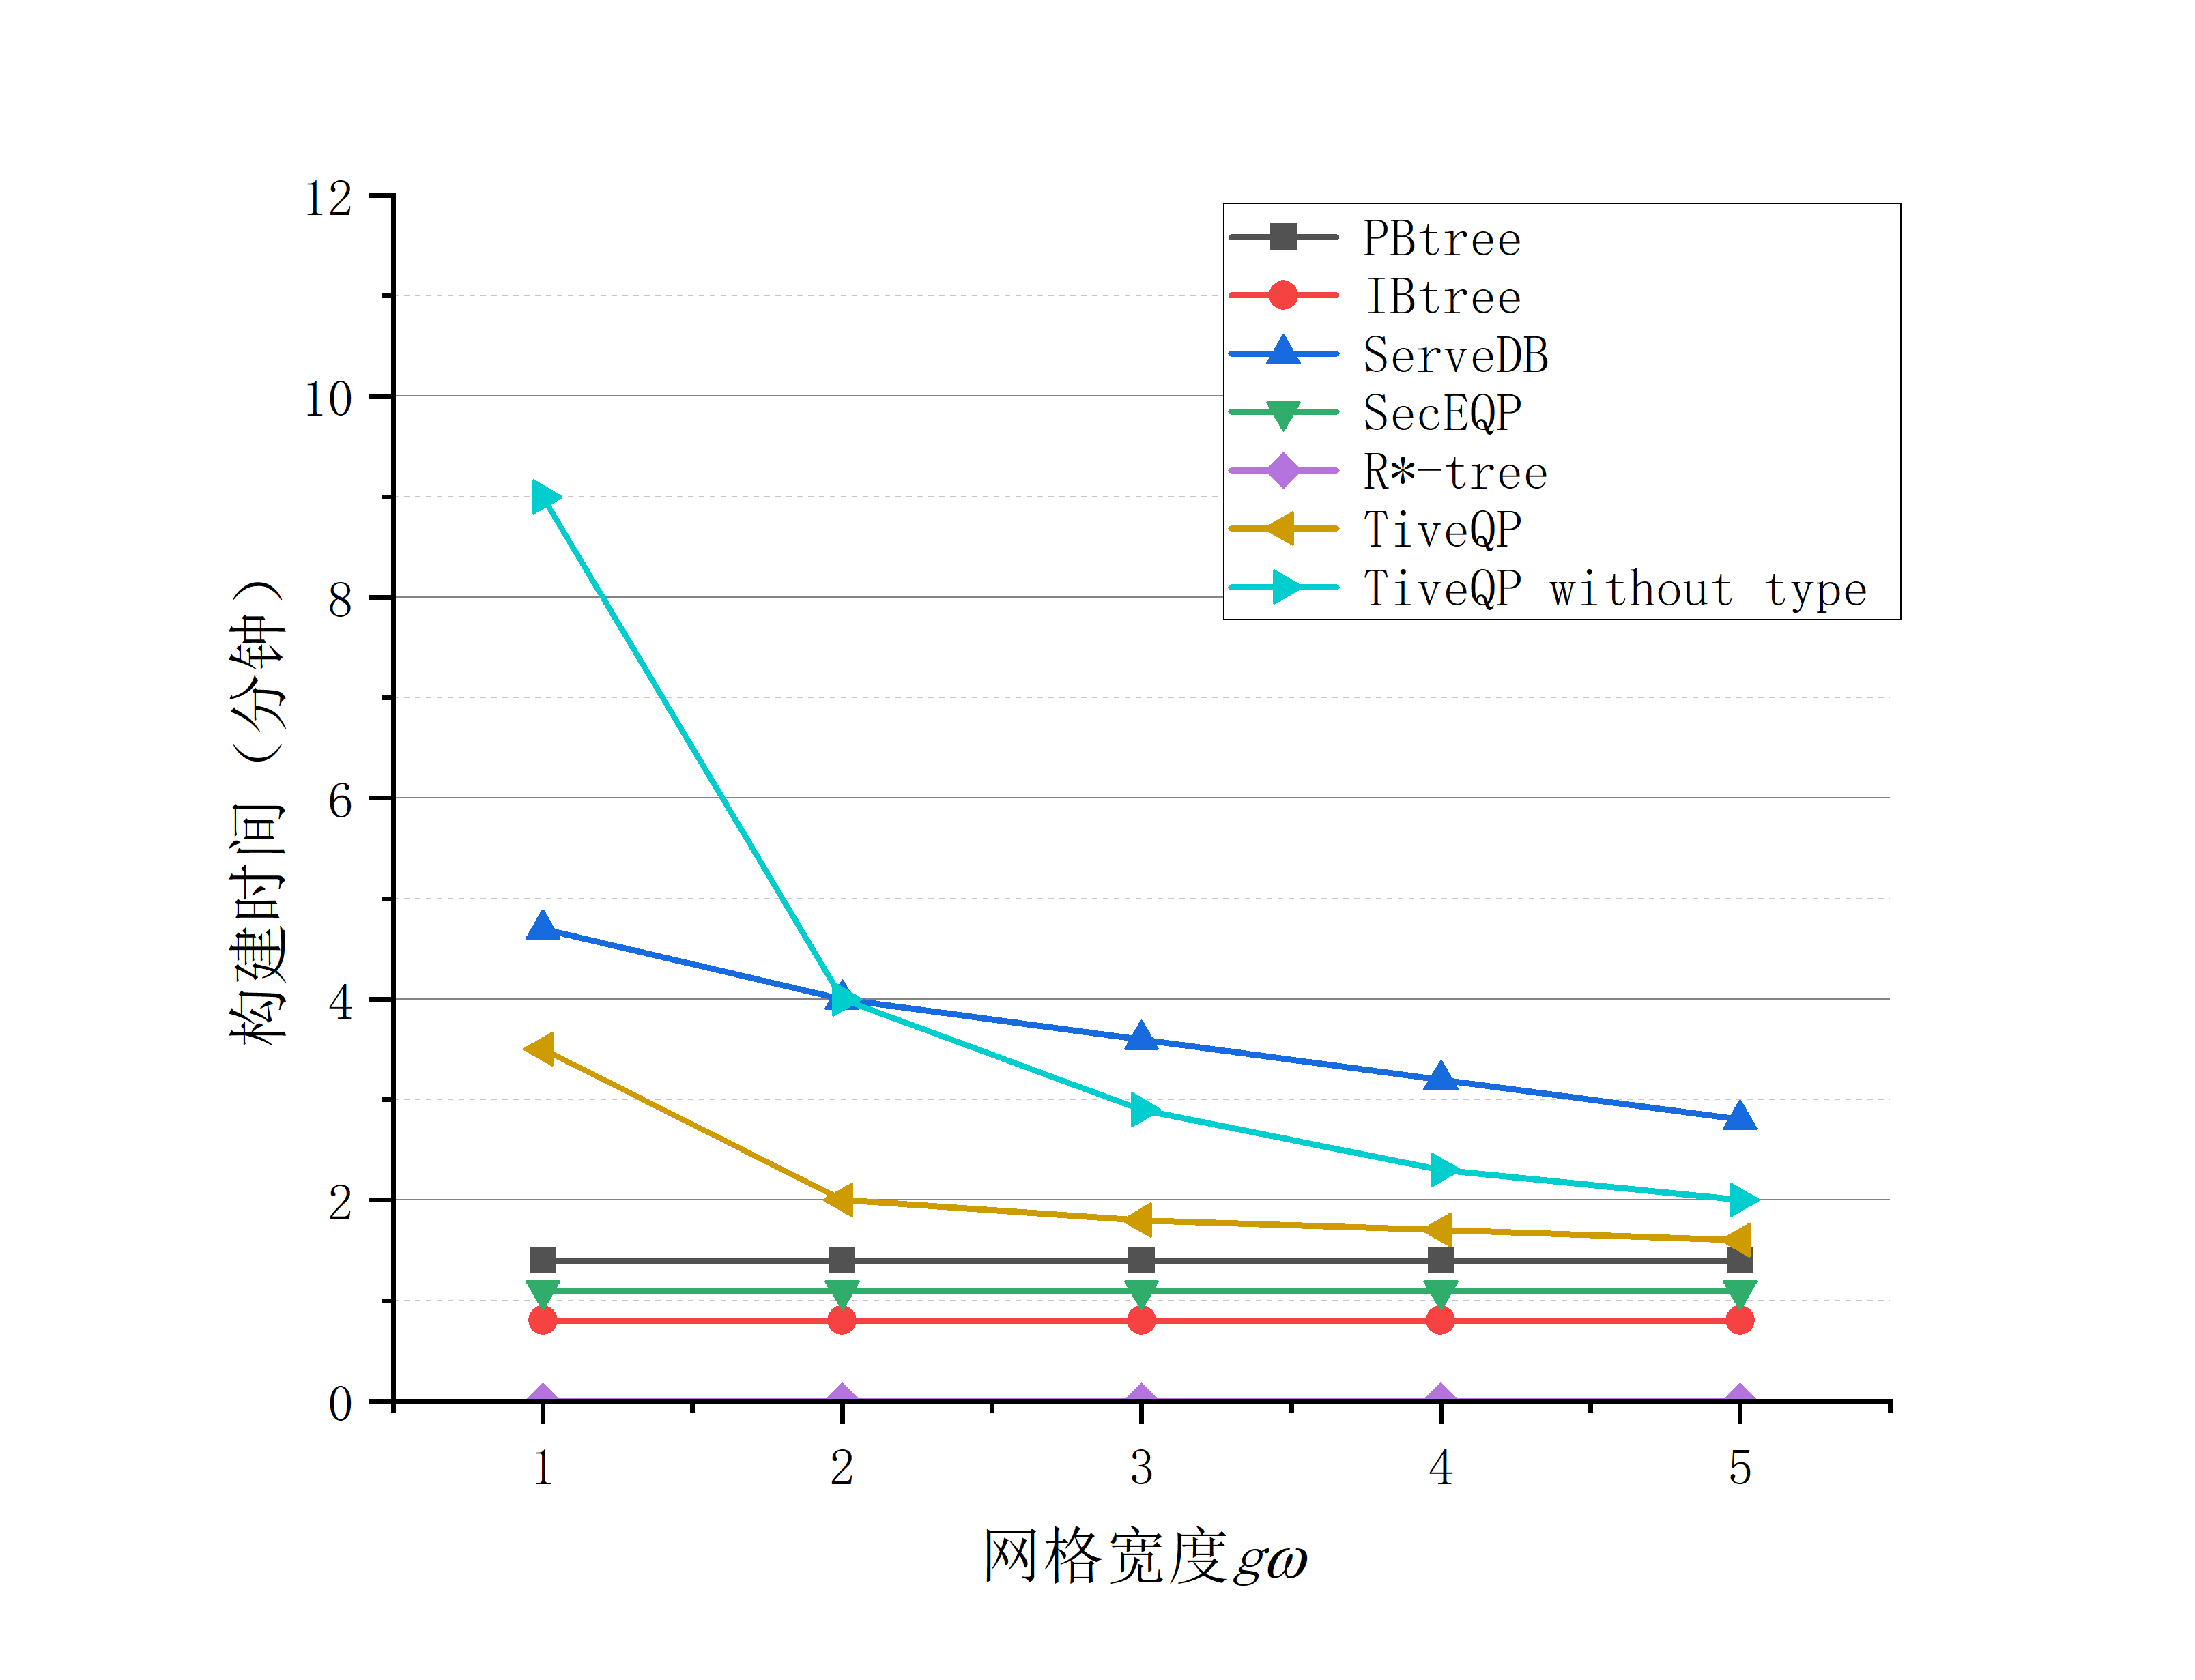
\includegraphics[width=0.45\textwidth]{jpgs/6-b.png}}
    \end{subcaptionbox}
    \centering
    \begin{subcaptionbox}{Index size varying \(n\)}
        {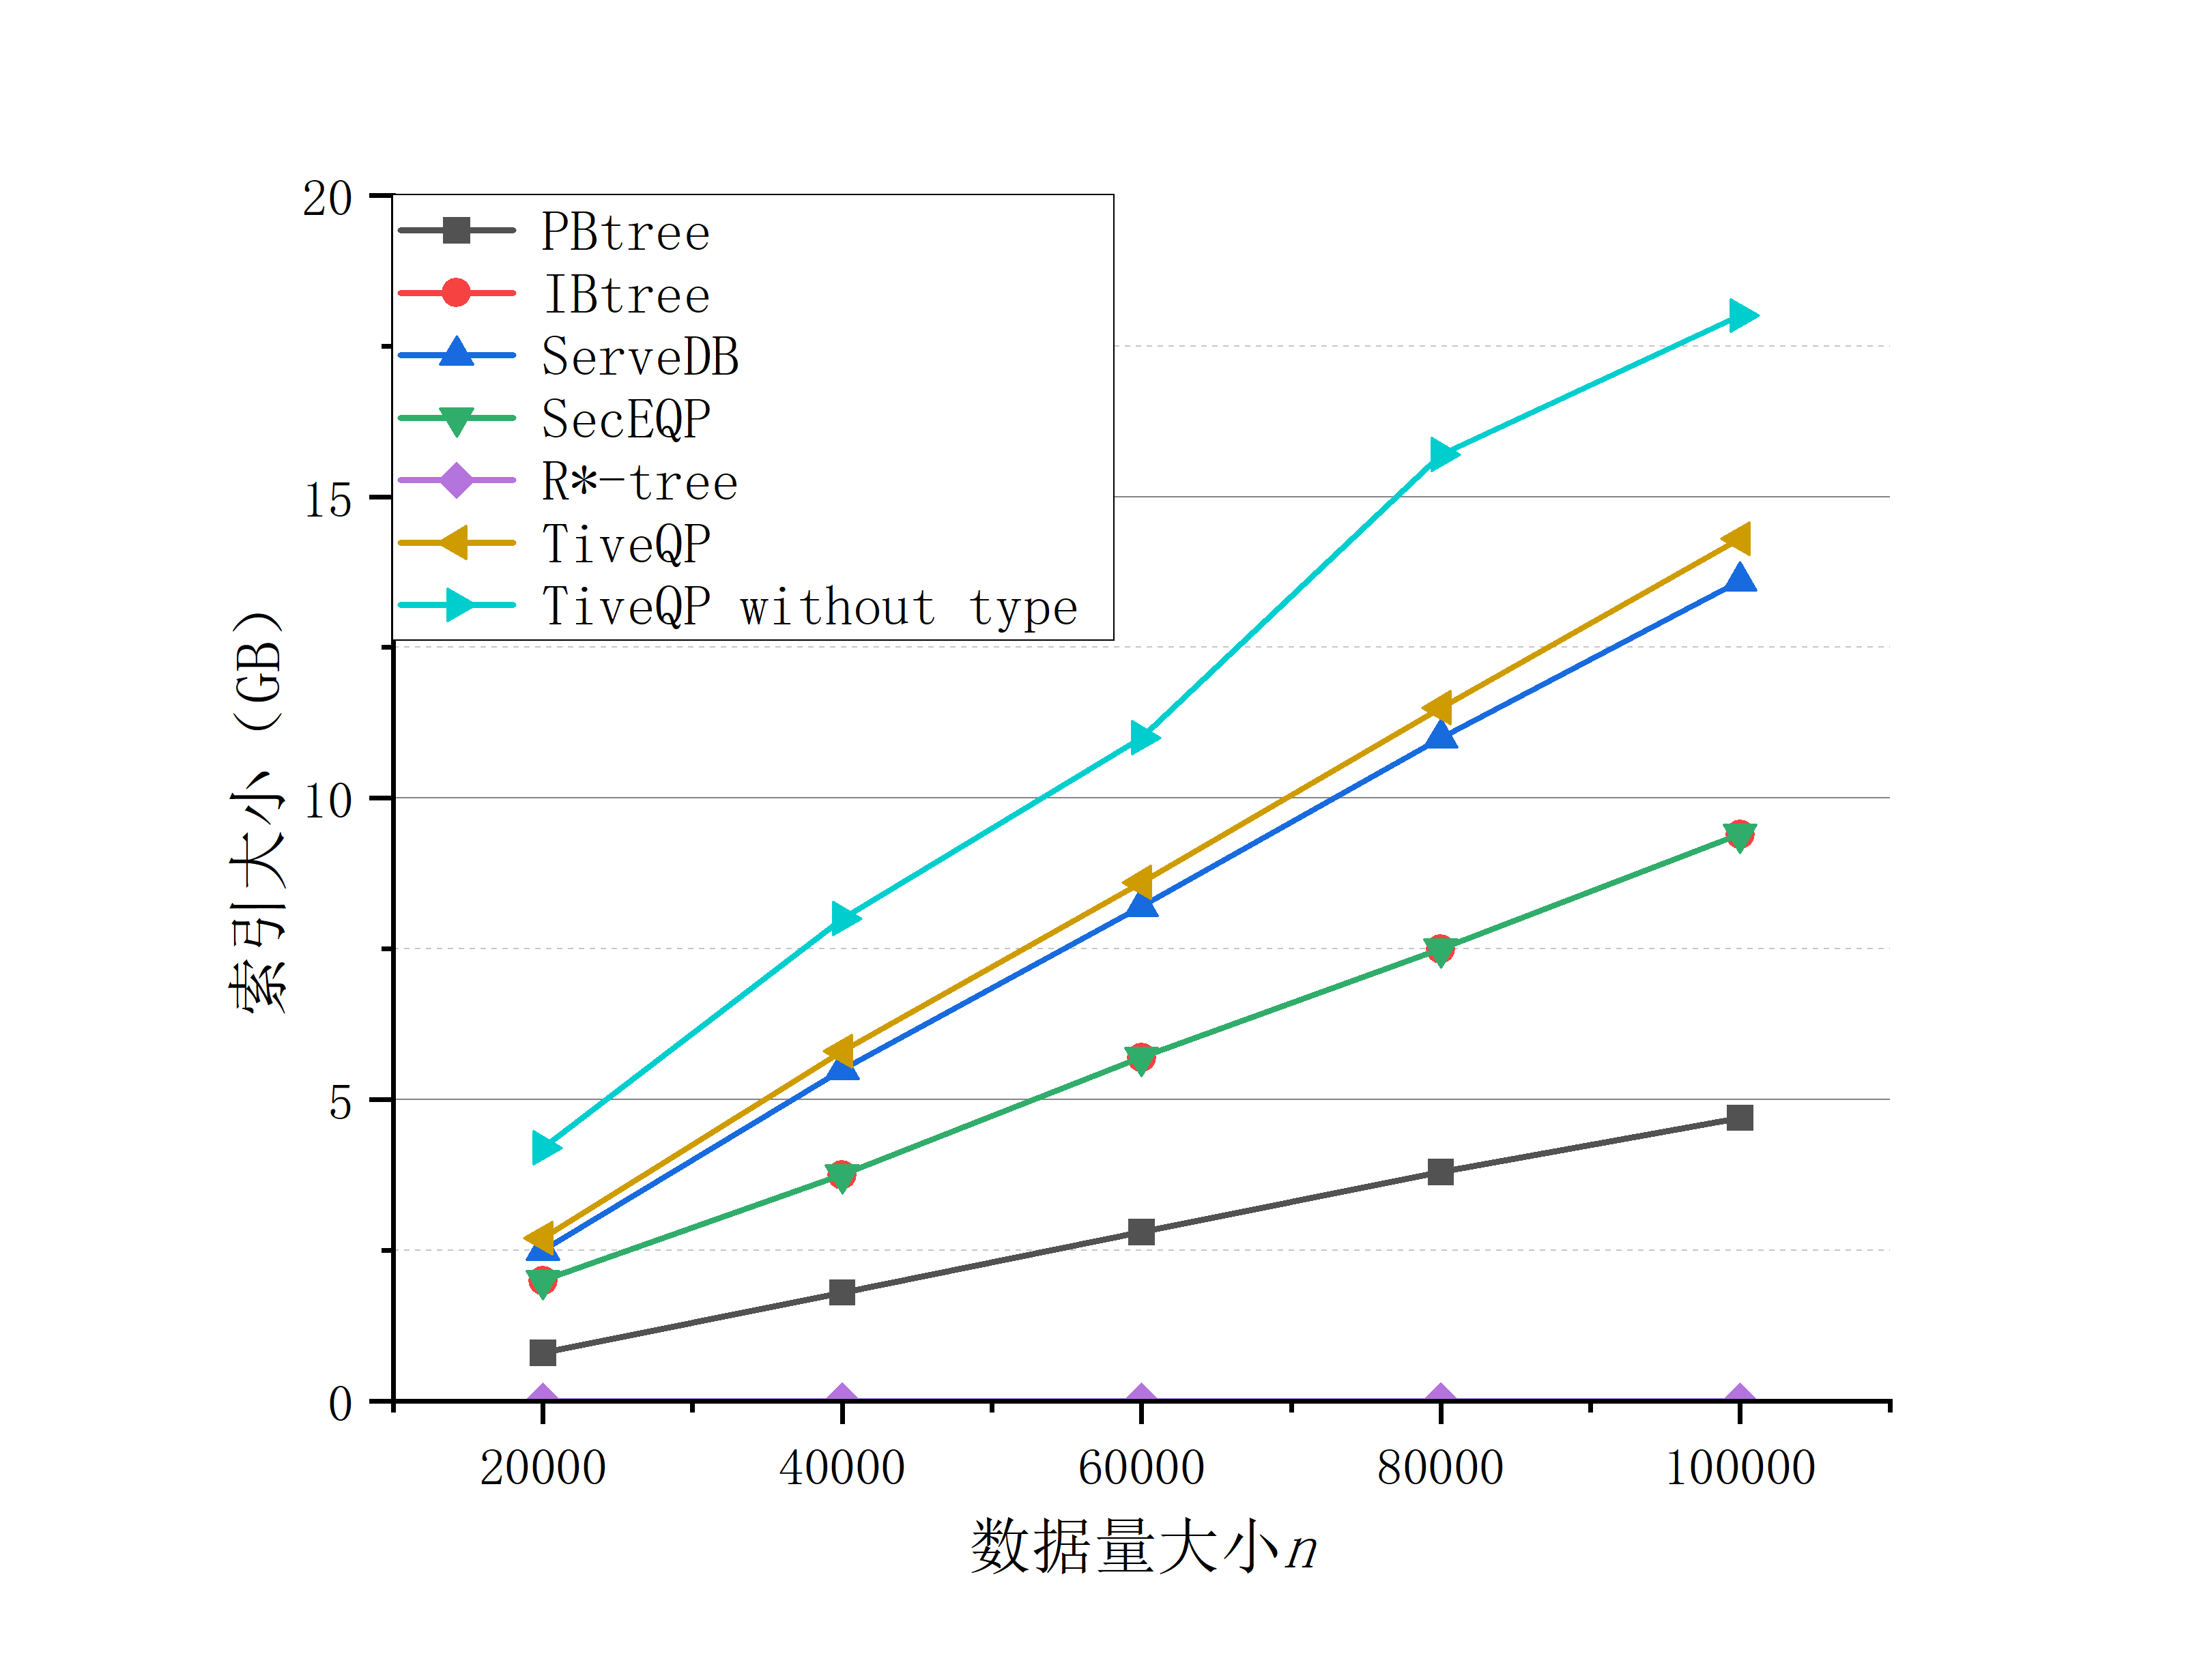
\includegraphics[width=0.45\textwidth]{jpgs/6-c.png}}
    \end{subcaptionbox}
    \hfill
    \begin{subcaptionbox}{Index size varying \(gw\)}
        {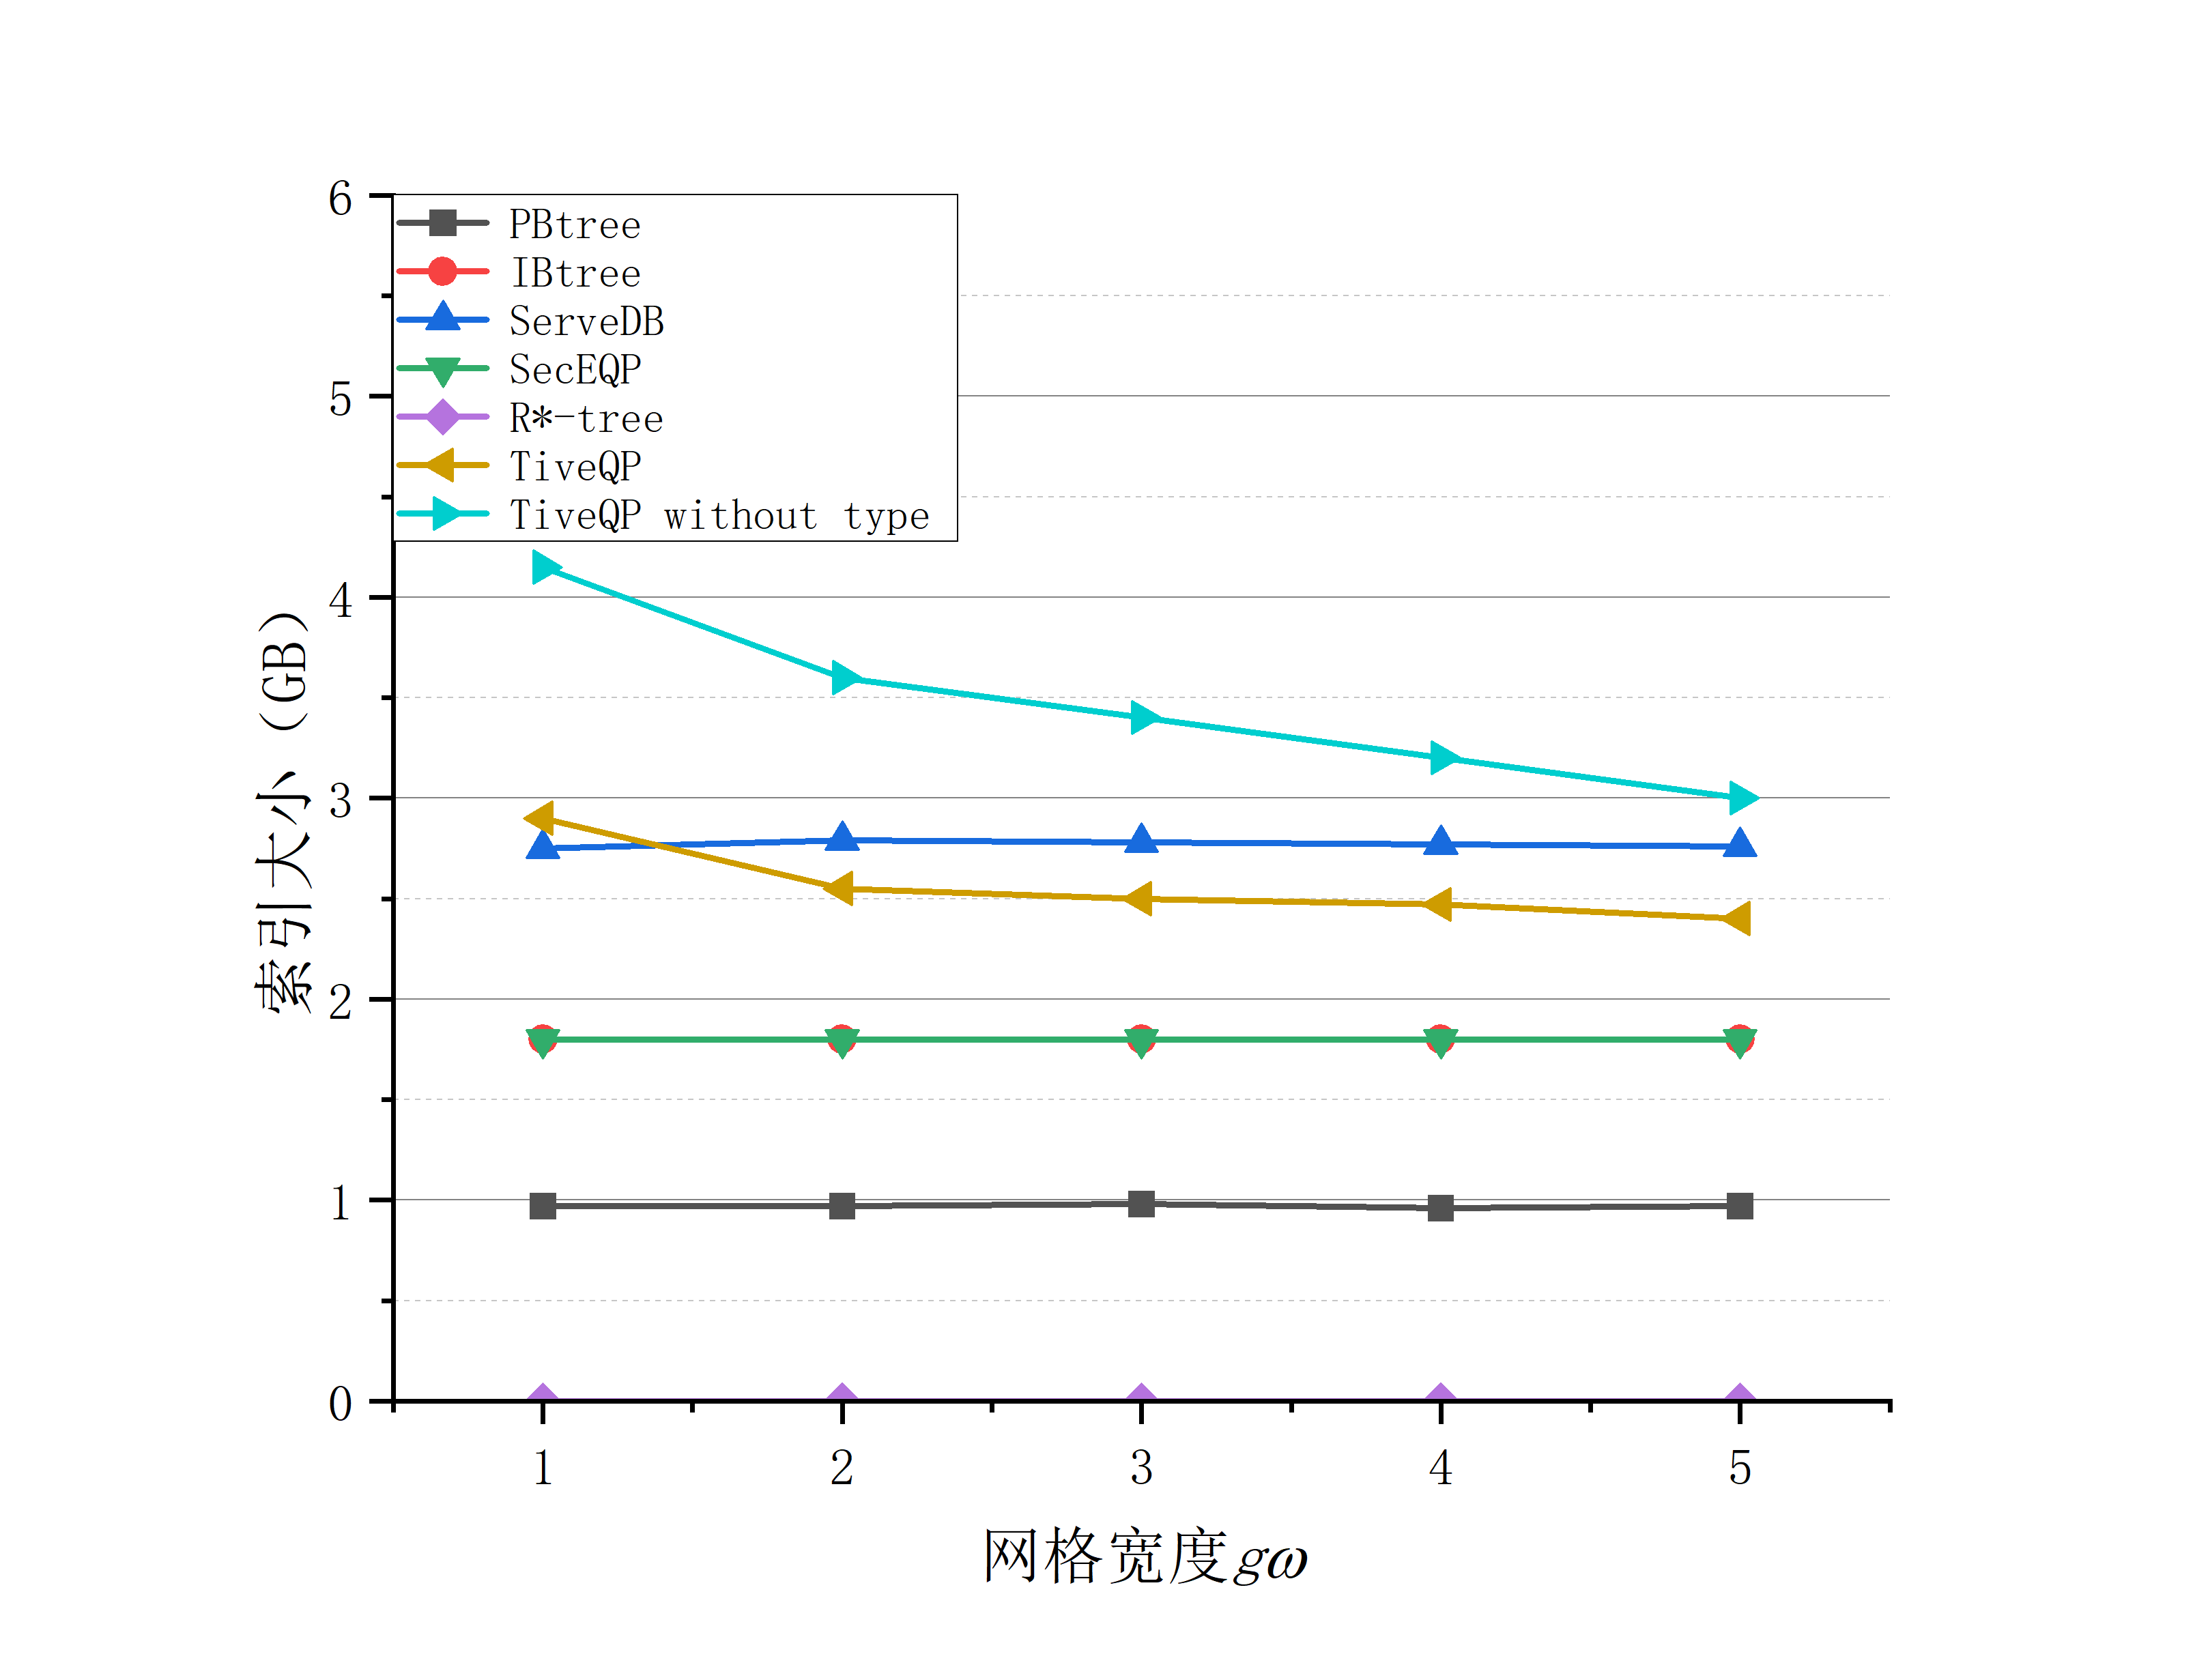
\includegraphics[width=0.45\textwidth]{jpgs/6-d.png}}
    \end{subcaptionbox}
    \caption{相关性能随 \(n\) 和 \(gw\) 的变化情况}
\end{figure}

关于不同的 \(n\) 和 \(gw\),树的大小分别从2.89GB增长到14.37GB,以及从2.89GB减少到2.34GB。

很明显,构建成本随着 \(n\) 的增加呈线性增长。而构建成本会随着位置宽度 \(gw\) 的增加而降低,这是因为当 \(gw\) 变大时,每个网格覆盖的空间更大,网格的数量会减少,从而减小了前缀最小集合(MS)的规模以及位置互补集合的规模。由于位(bits)和哈希值向量(Hv)的总长度比布隆过滤器(IBF)短得多,所以 \(gw\) 对树构建的影响较小。

我们注意到,在图5.1(b)中最左边的绿色点迅速下降到下一个点。这是因为当 \(gw\) 从1增加到2时,两个相应互补集合的规模差异比之后的互补集合规模差异更大,这就导致了更多的哈希运算。

验证信息的生成在构建时间中占主导地位,因为我们需要计算每个节点的互补集合,然后再计算位(bits)和哈希值向量(Hv)。这些计算比在叶子节点上对布隆过滤器(IBF)进行的哈希运算消耗的时间更多。

一个布隆过滤器(IBF)的大小对应于插入到该布隆过滤器中的前缀的总数。布隆过滤器(IBF)决定了树的大小。例如,当 \(n = 20,000\) 且 \(gw = 1\) 千米时,树的大小为2.893GB,而布隆过滤器(IBF)的大小为1.863GB。这是因为:
\begin{enumerate}
    \item 在给定固定的 \(n\) 和 \(m\) 的情况下,为了维持误报率(FPR),一个布隆过滤器(IBF)的长度会比较长;
    \item 对于一个叶子节点,其三个互补集合中的每一个都会生成一个较小的前缀族集合,这使得通信开销较小,并且随着节点向上合并,这三个互补集合会变得更小;
    \item 位(bits)中的每个字符串都有 \(m\) 个位以及一个标识符,哈希消息认证码集合(Sv)中的元素和哈希值(HV)都是256位。
\end{enumerate}
实验结果表明,TiveTree的构建成本是可以接受的。

\subsubsection{检索耗时}
查询处理的时间复杂度为 \(O(k\log(\frac{n}{k}))\) 。平均时间:图5.2(a)到5.2(c)分别展示了关于不同的 \(n\)、位置宽度 \(gw\) 和 \(k\) 的查询延迟(假设插入相关图片,示例同构建耗时部分图片插入方式)。实验结果表明,查询处理时间在毫秒量级。



\begin{figure}[h]
    \centering
    \begin{subcaptionbox}{Average query time by varying \(n\)}
        {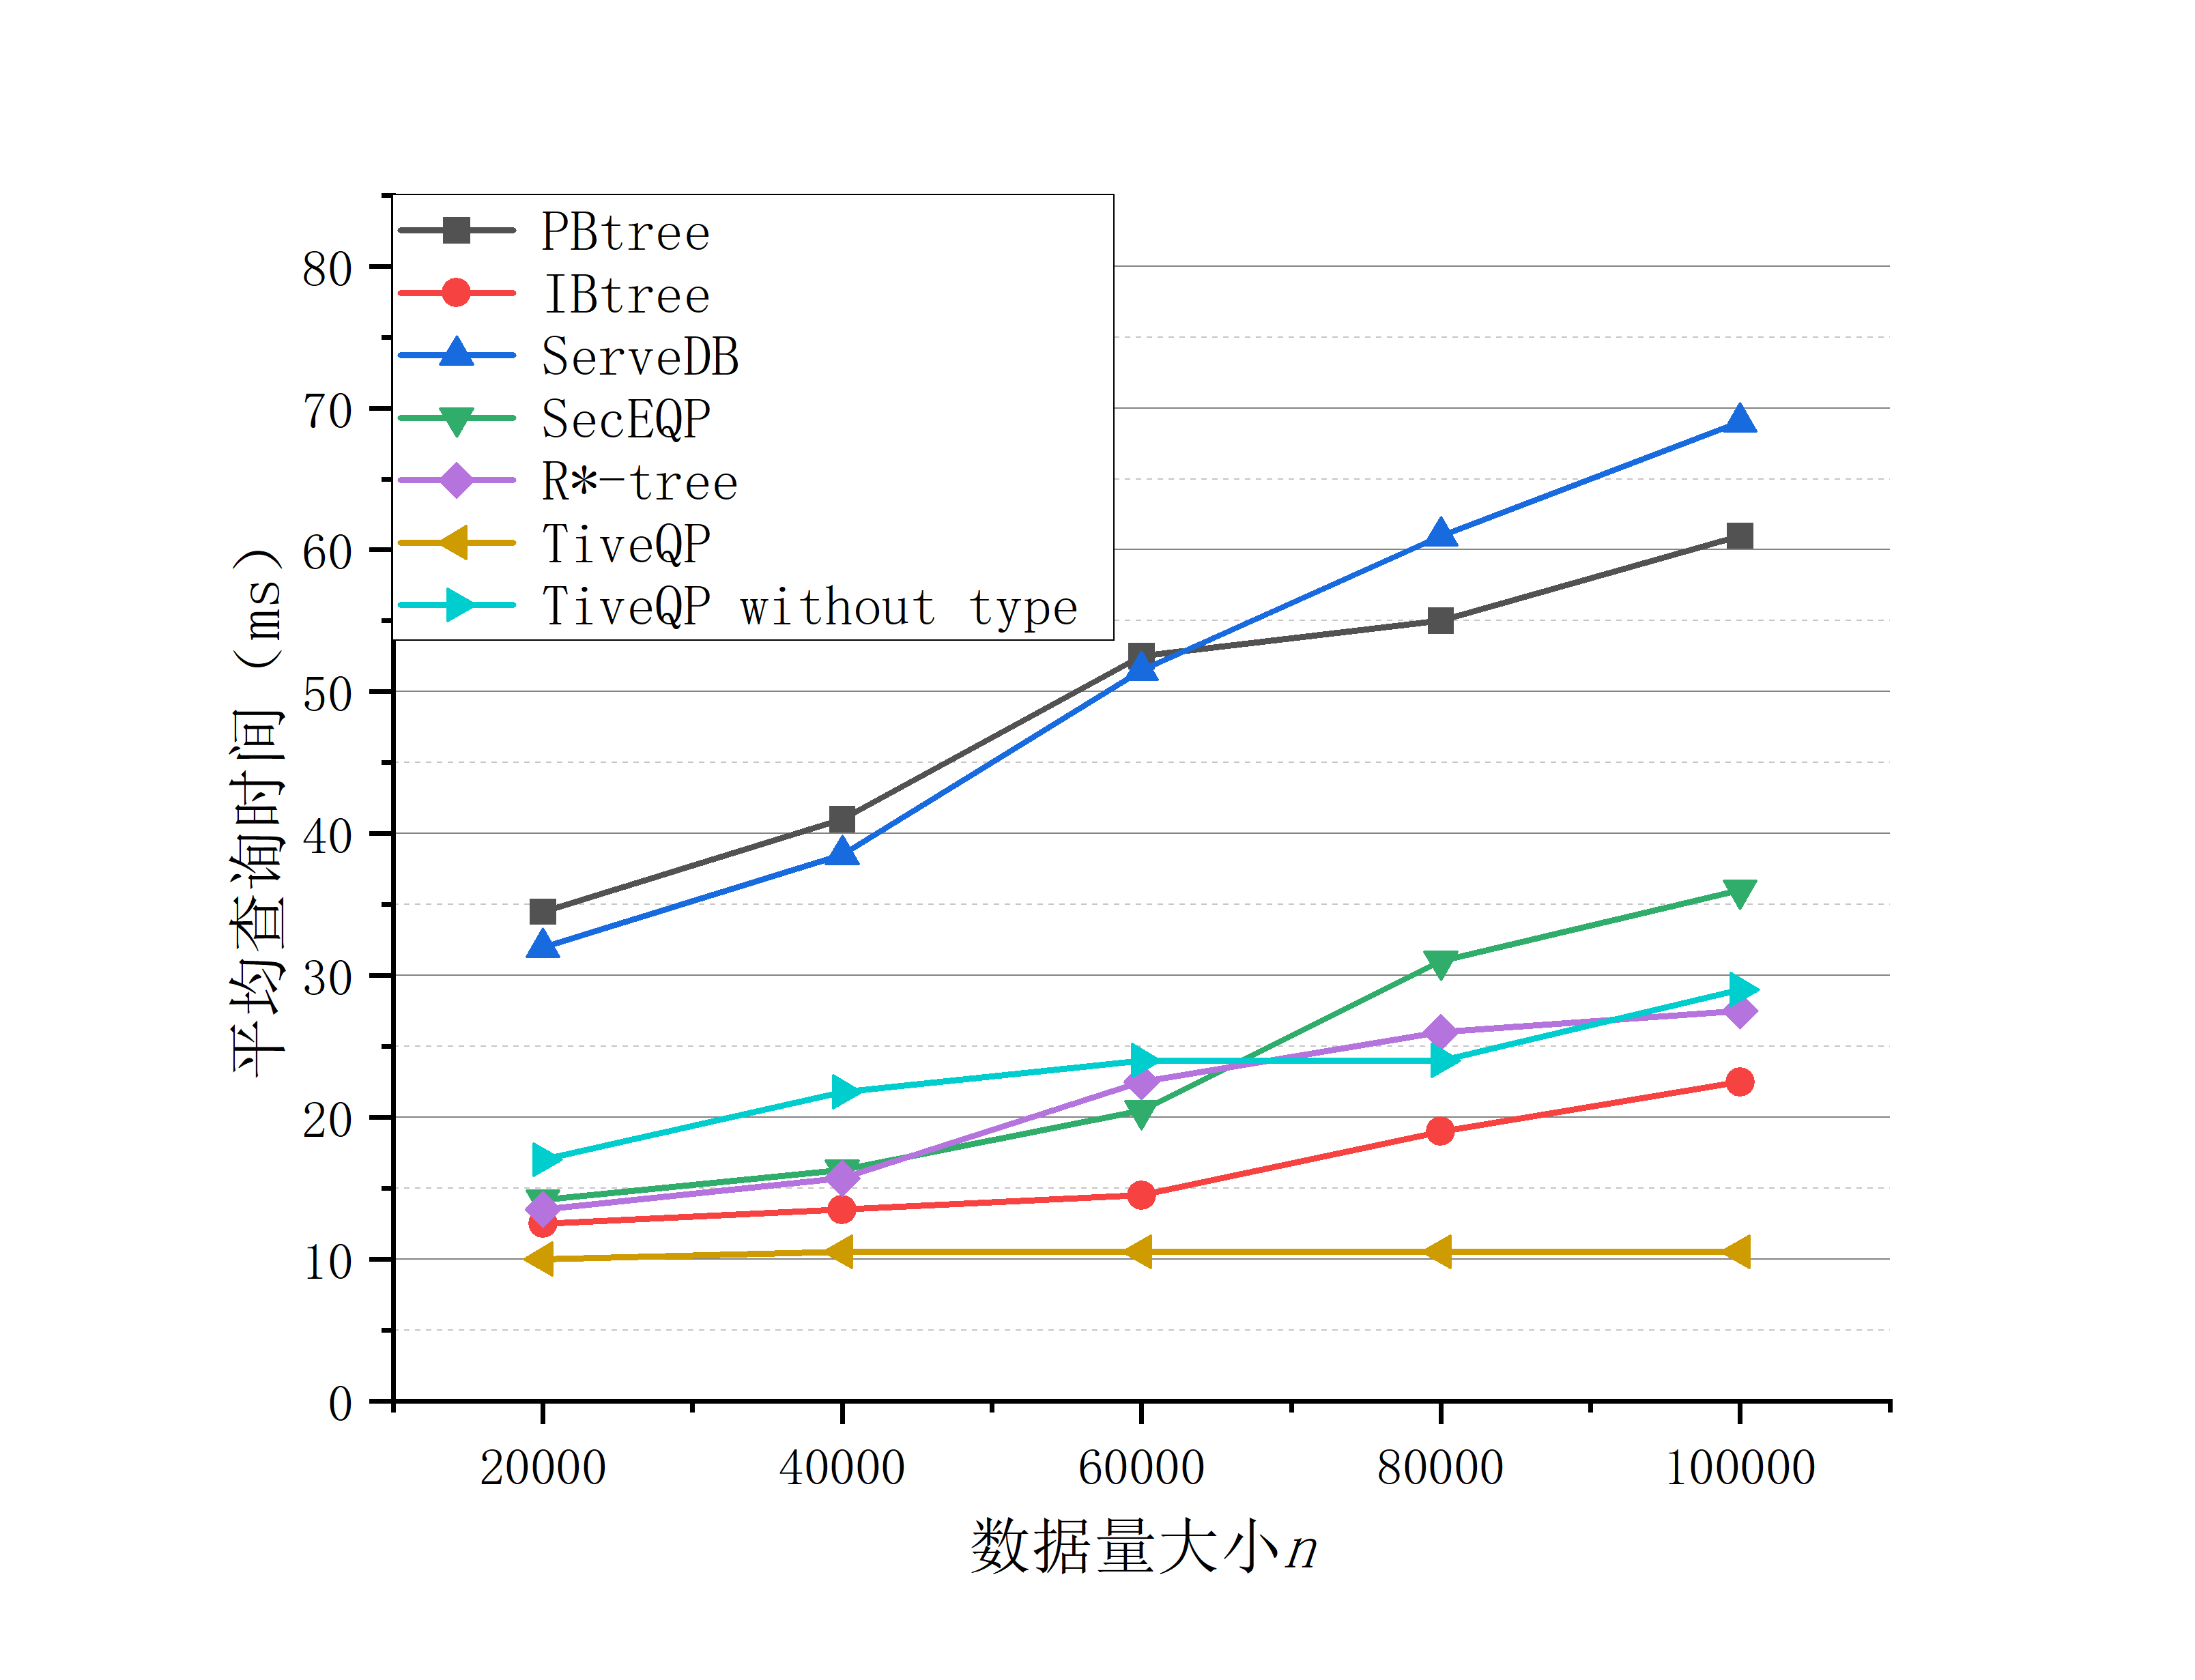
\includegraphics[width=0.3\textwidth]{jpgs/7-a.png}}
    \end{subcaptionbox}
    \hspace{10pt}
    \begin{subcaptionbox}{Average query time varying \(gw\)}
        {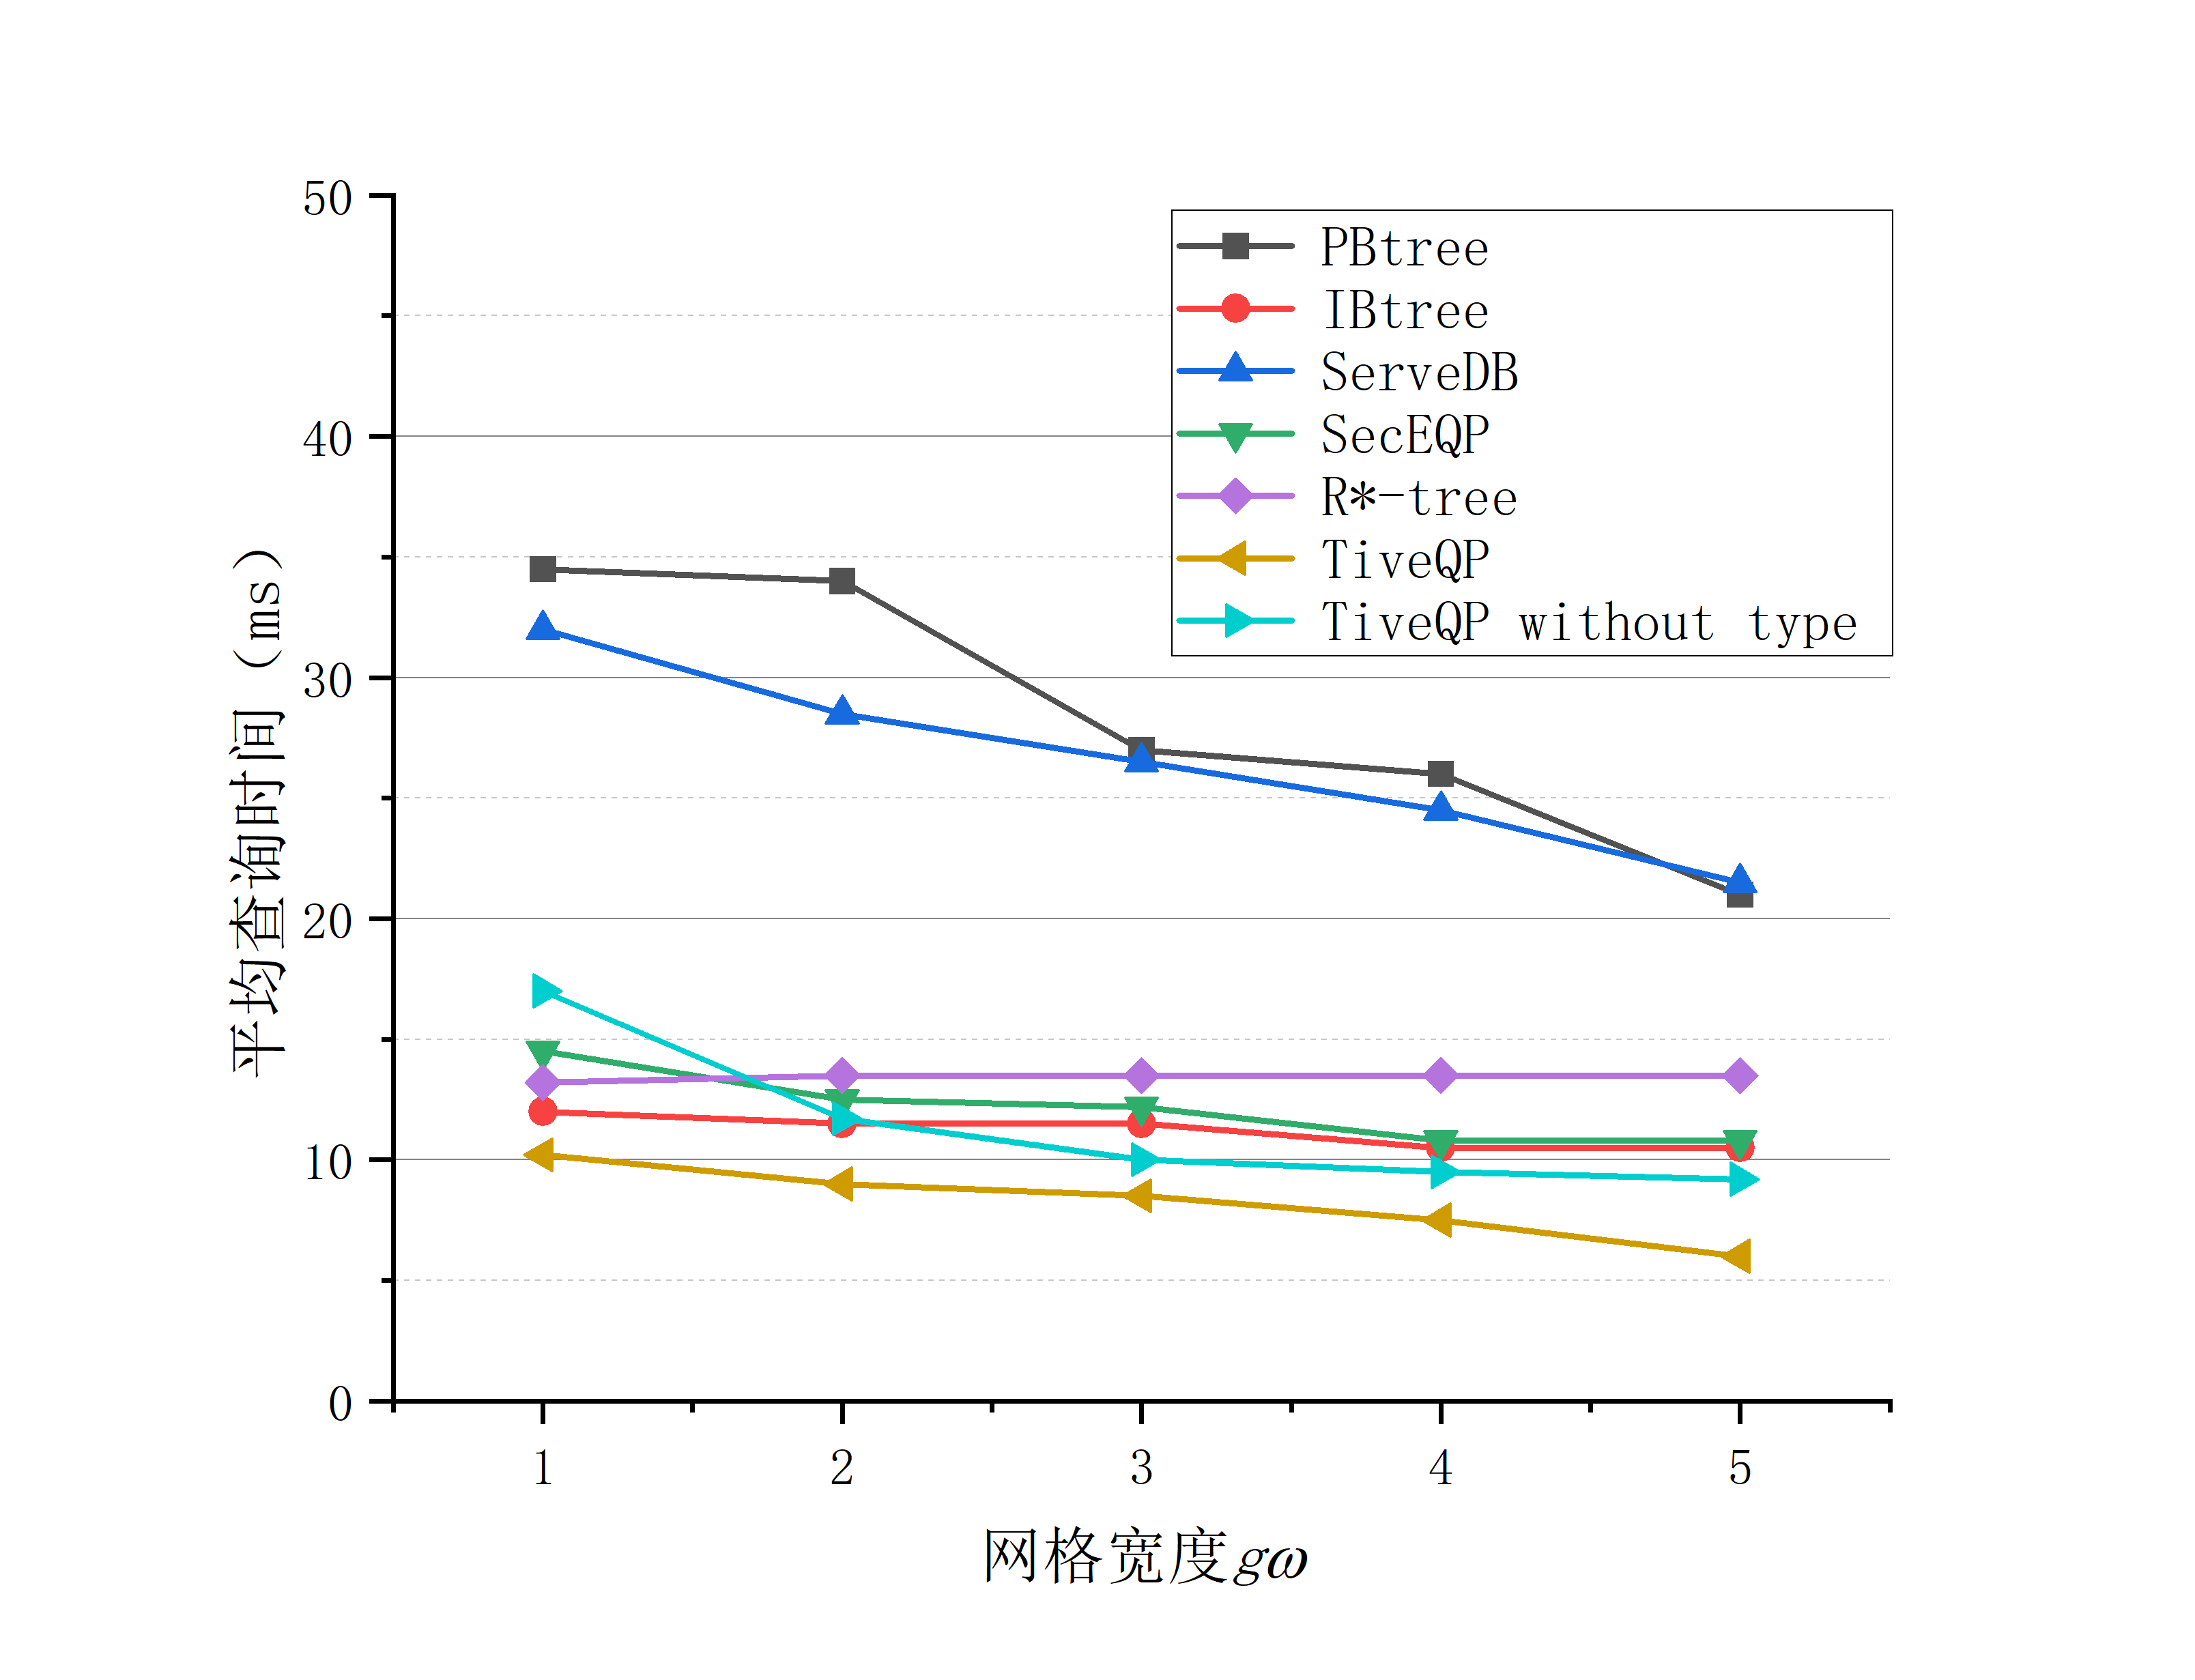
\includegraphics[width=0.3\textwidth]{jpgs/7-b.png}}
    \end{subcaptionbox}
    \hspace{10pt}
    \begin{subcaptionbox}{Average query time varying \(k\)}
        {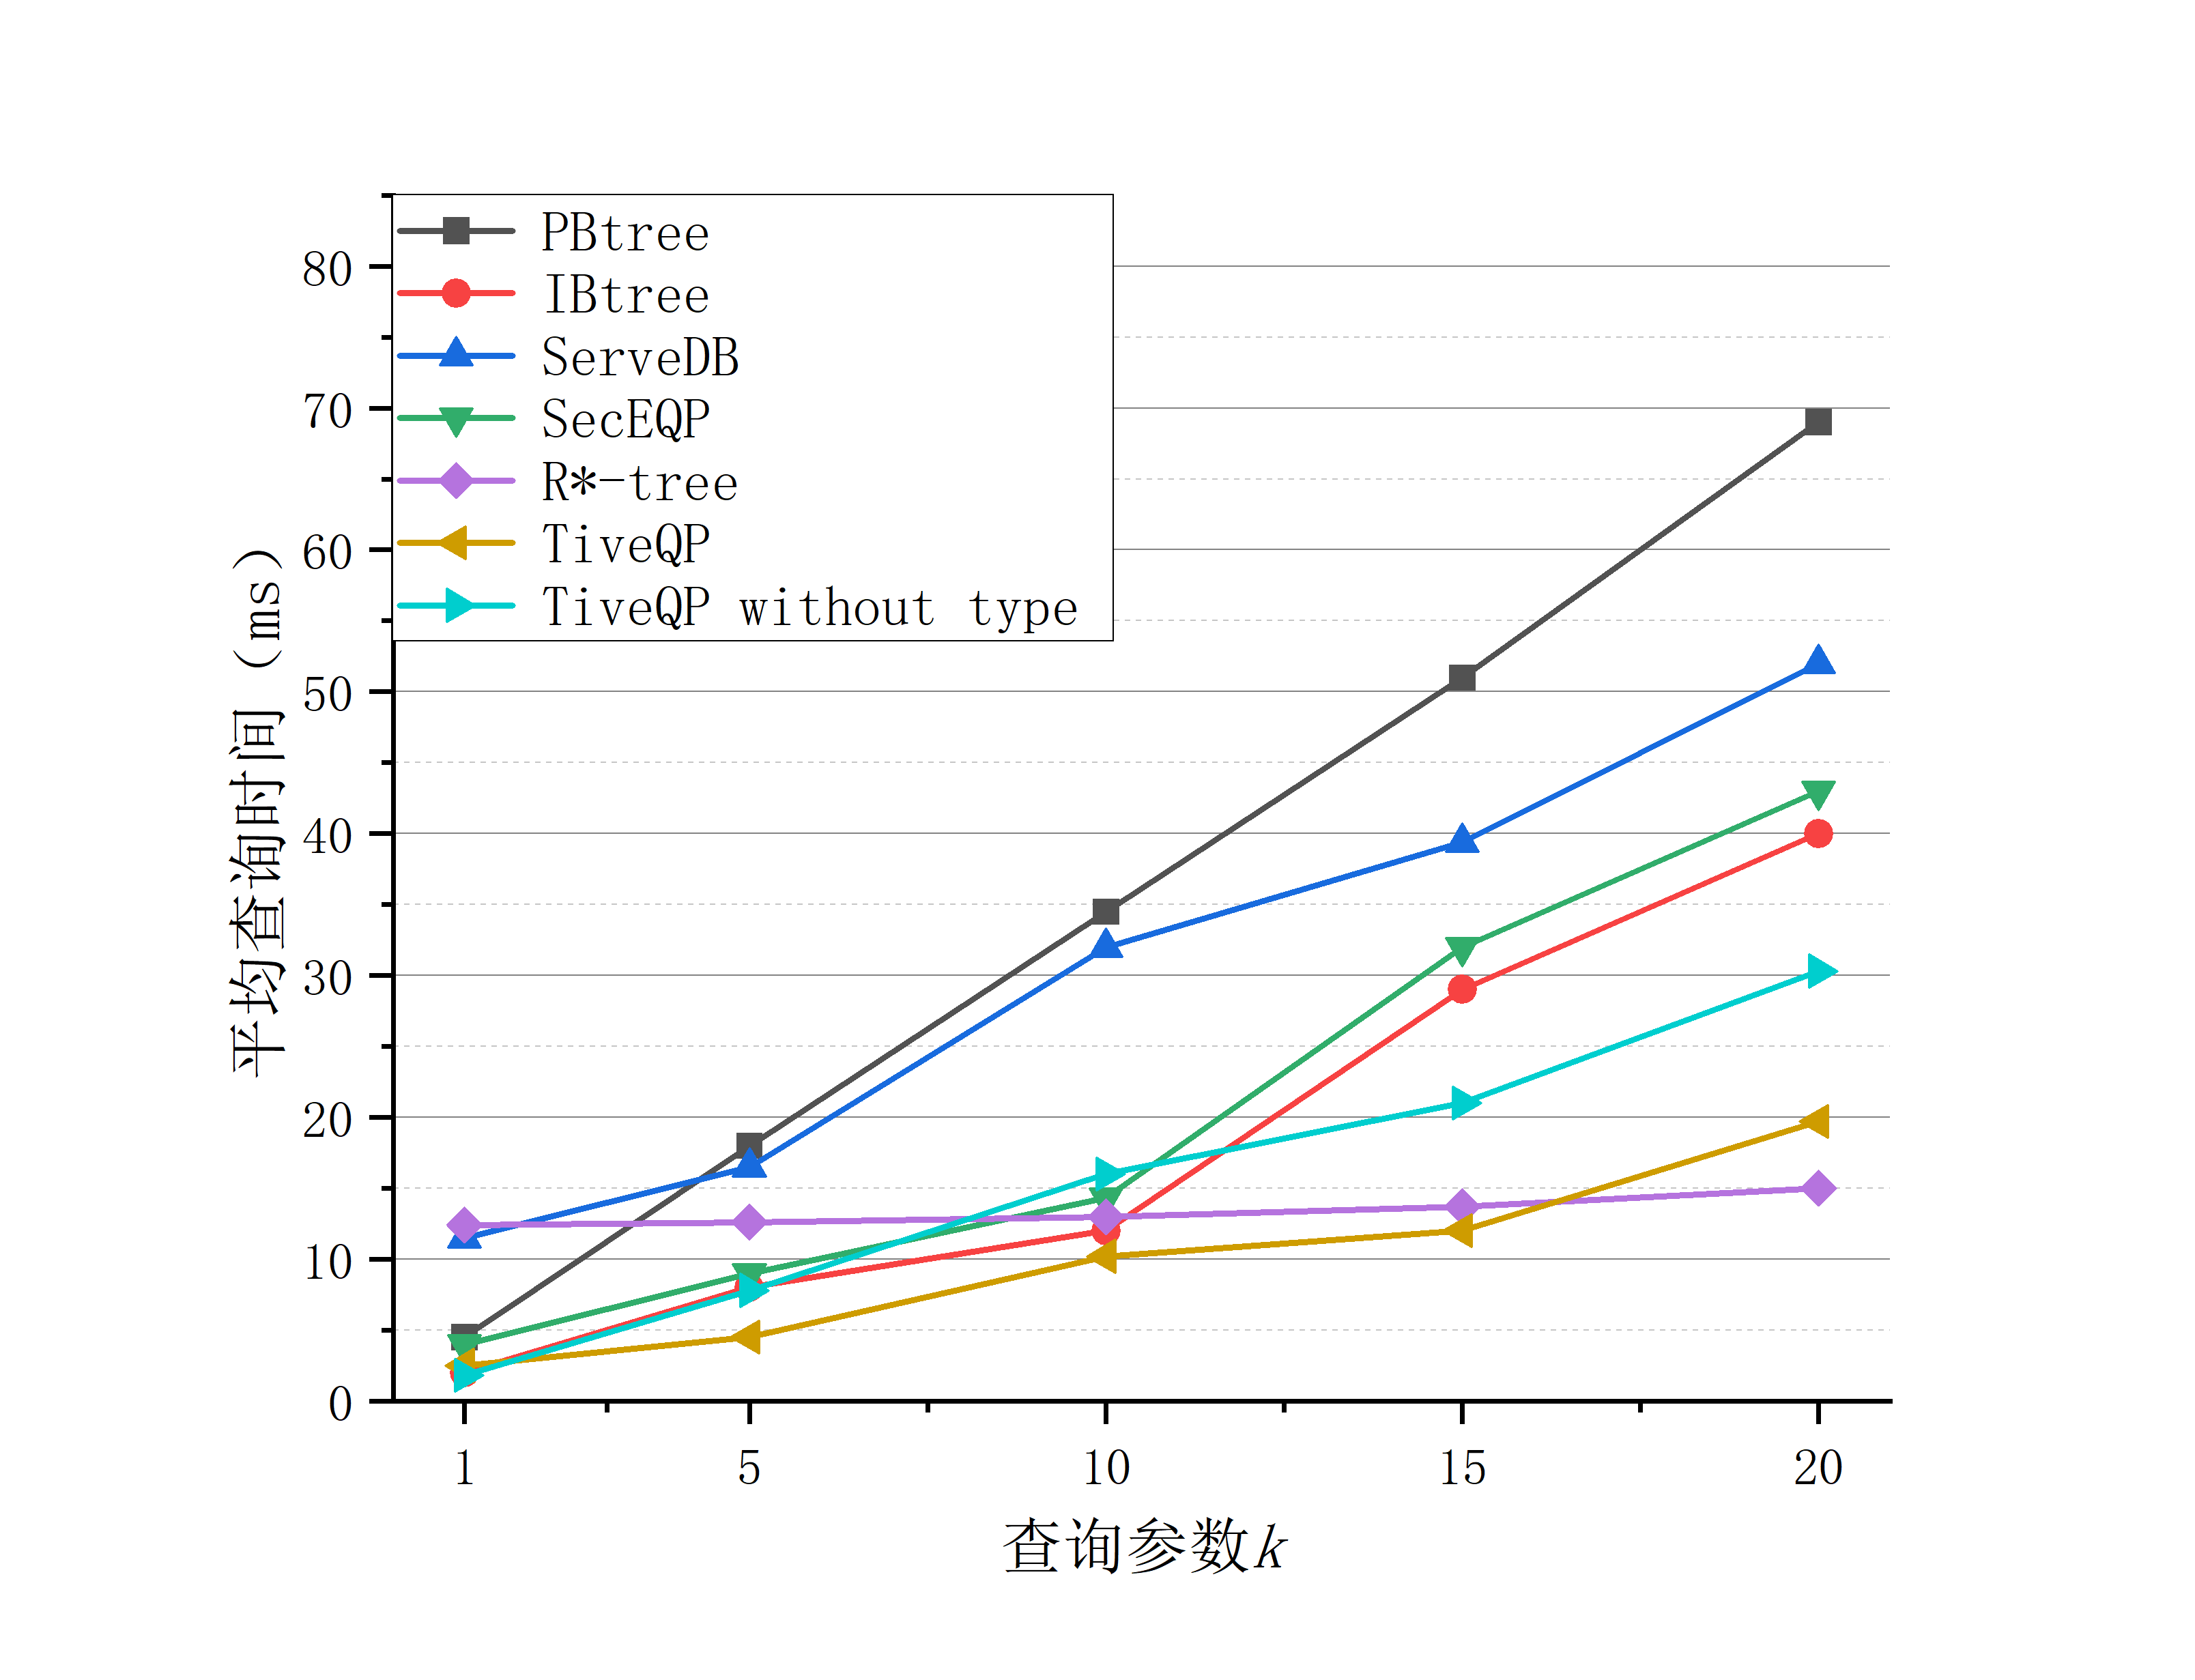
\includegraphics[width=0.3\textwidth]{jpgs/7-c.png}}
    \end{subcaptionbox}
    \caption{平均查询时间随不同参数的变化情况}
    \label{fig:query_time}
\end{figure}

改变 \(gw\):当 \(n = 20,000\) 且 \(k = 10\) 时,TiveQP的平均查询处理时间约为10毫秒。它不会随 \(n\) 增加,原因有两点:
\begin{enumerate}
    \item 我们在五个集合中使用所有数据项进行查询,因此它们的总数保持不变;
    \item 在按照类型和城市组织树之后,所需的数据项被排列在叶子节点附近,即它们被放置在索引树的一个小的子树中。 
\end{enumerate}
当 \(n = 20,000\) 且 \(k = 10\) 时,随着网格宽度 \(gw\) 从1千米增加到5千米,平均查询处理时间从10.1毫秒减少到6.2毫秒。出现这种情况是因为随着 \(gw\) 增加,位置前缀数量中的陷阱门变得更少,这导致更少的哈希操作,进而减少处理时间。

改变 \(k\):当 \(n = 20,000\) 且 \(gw = 1\) 时,随着 \(k\) 从1增加到20,平均查询处理时间从2.5毫秒增长到19.8毫秒。这是显而易见的,因为更多的查询会导致更多的搜索路径和时间。

\subsubsection{验证耗时}
数据用户会验证结果的正确性和完整性。我们记录了关于 \(n\)、位置宽度 \(gw\) 和 \(k\) 的平均验证时间。图5.3(a)、图5.3(b)和图5.3(c)表明,该时间在 \(n\) 和 \(gw\) 变化时几乎保持不变(假设插入相关图片)。我们将此优势归因于,在精心进行结构组织后,TiveQP才构建索引树。随着 \(k\) 的增加,时间会略有增长,因为用户必须检查更多搜索路径的更多证明。

\begin{figure}[h]
    \centering
    \begin{subcaptionbox}{Average verification time varying \(n\)}
        {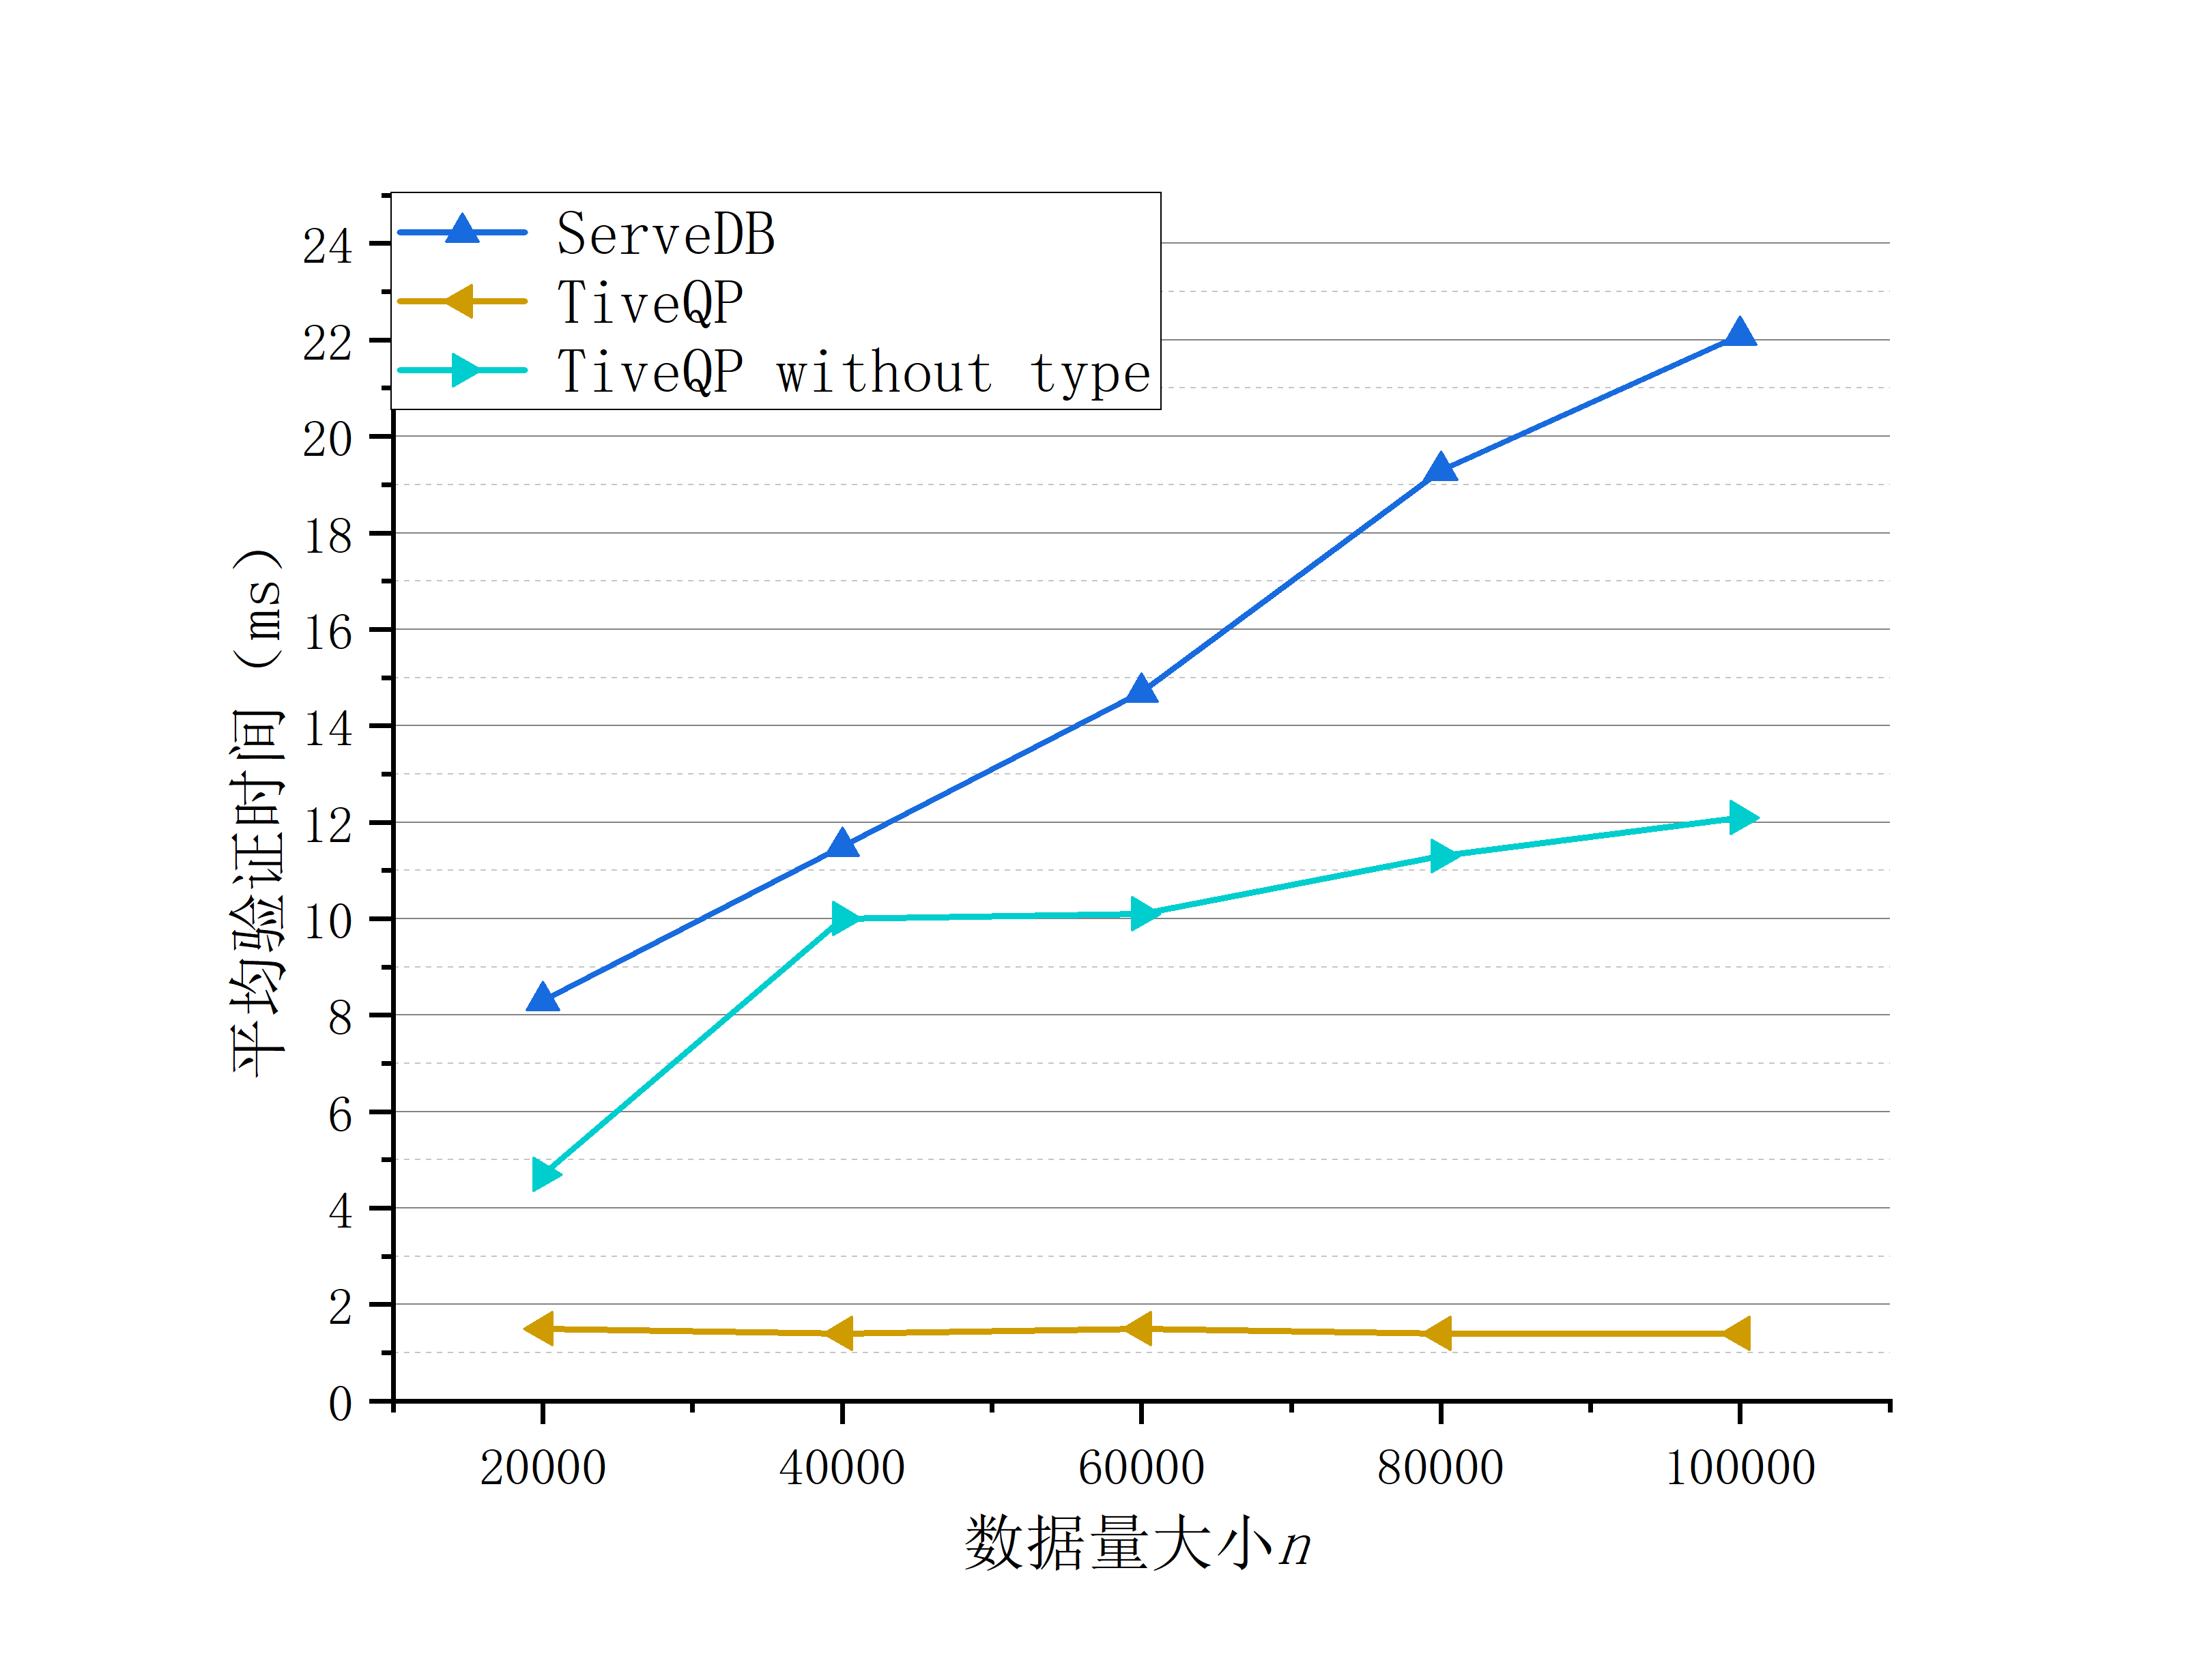
\includegraphics[width=0.3\textwidth]{jpgs/8-a.png}}
    \end{subcaptionbox}
    \hspace{10pt}
    \begin{subcaptionbox}{Average verification time varying \(gw\)}
        {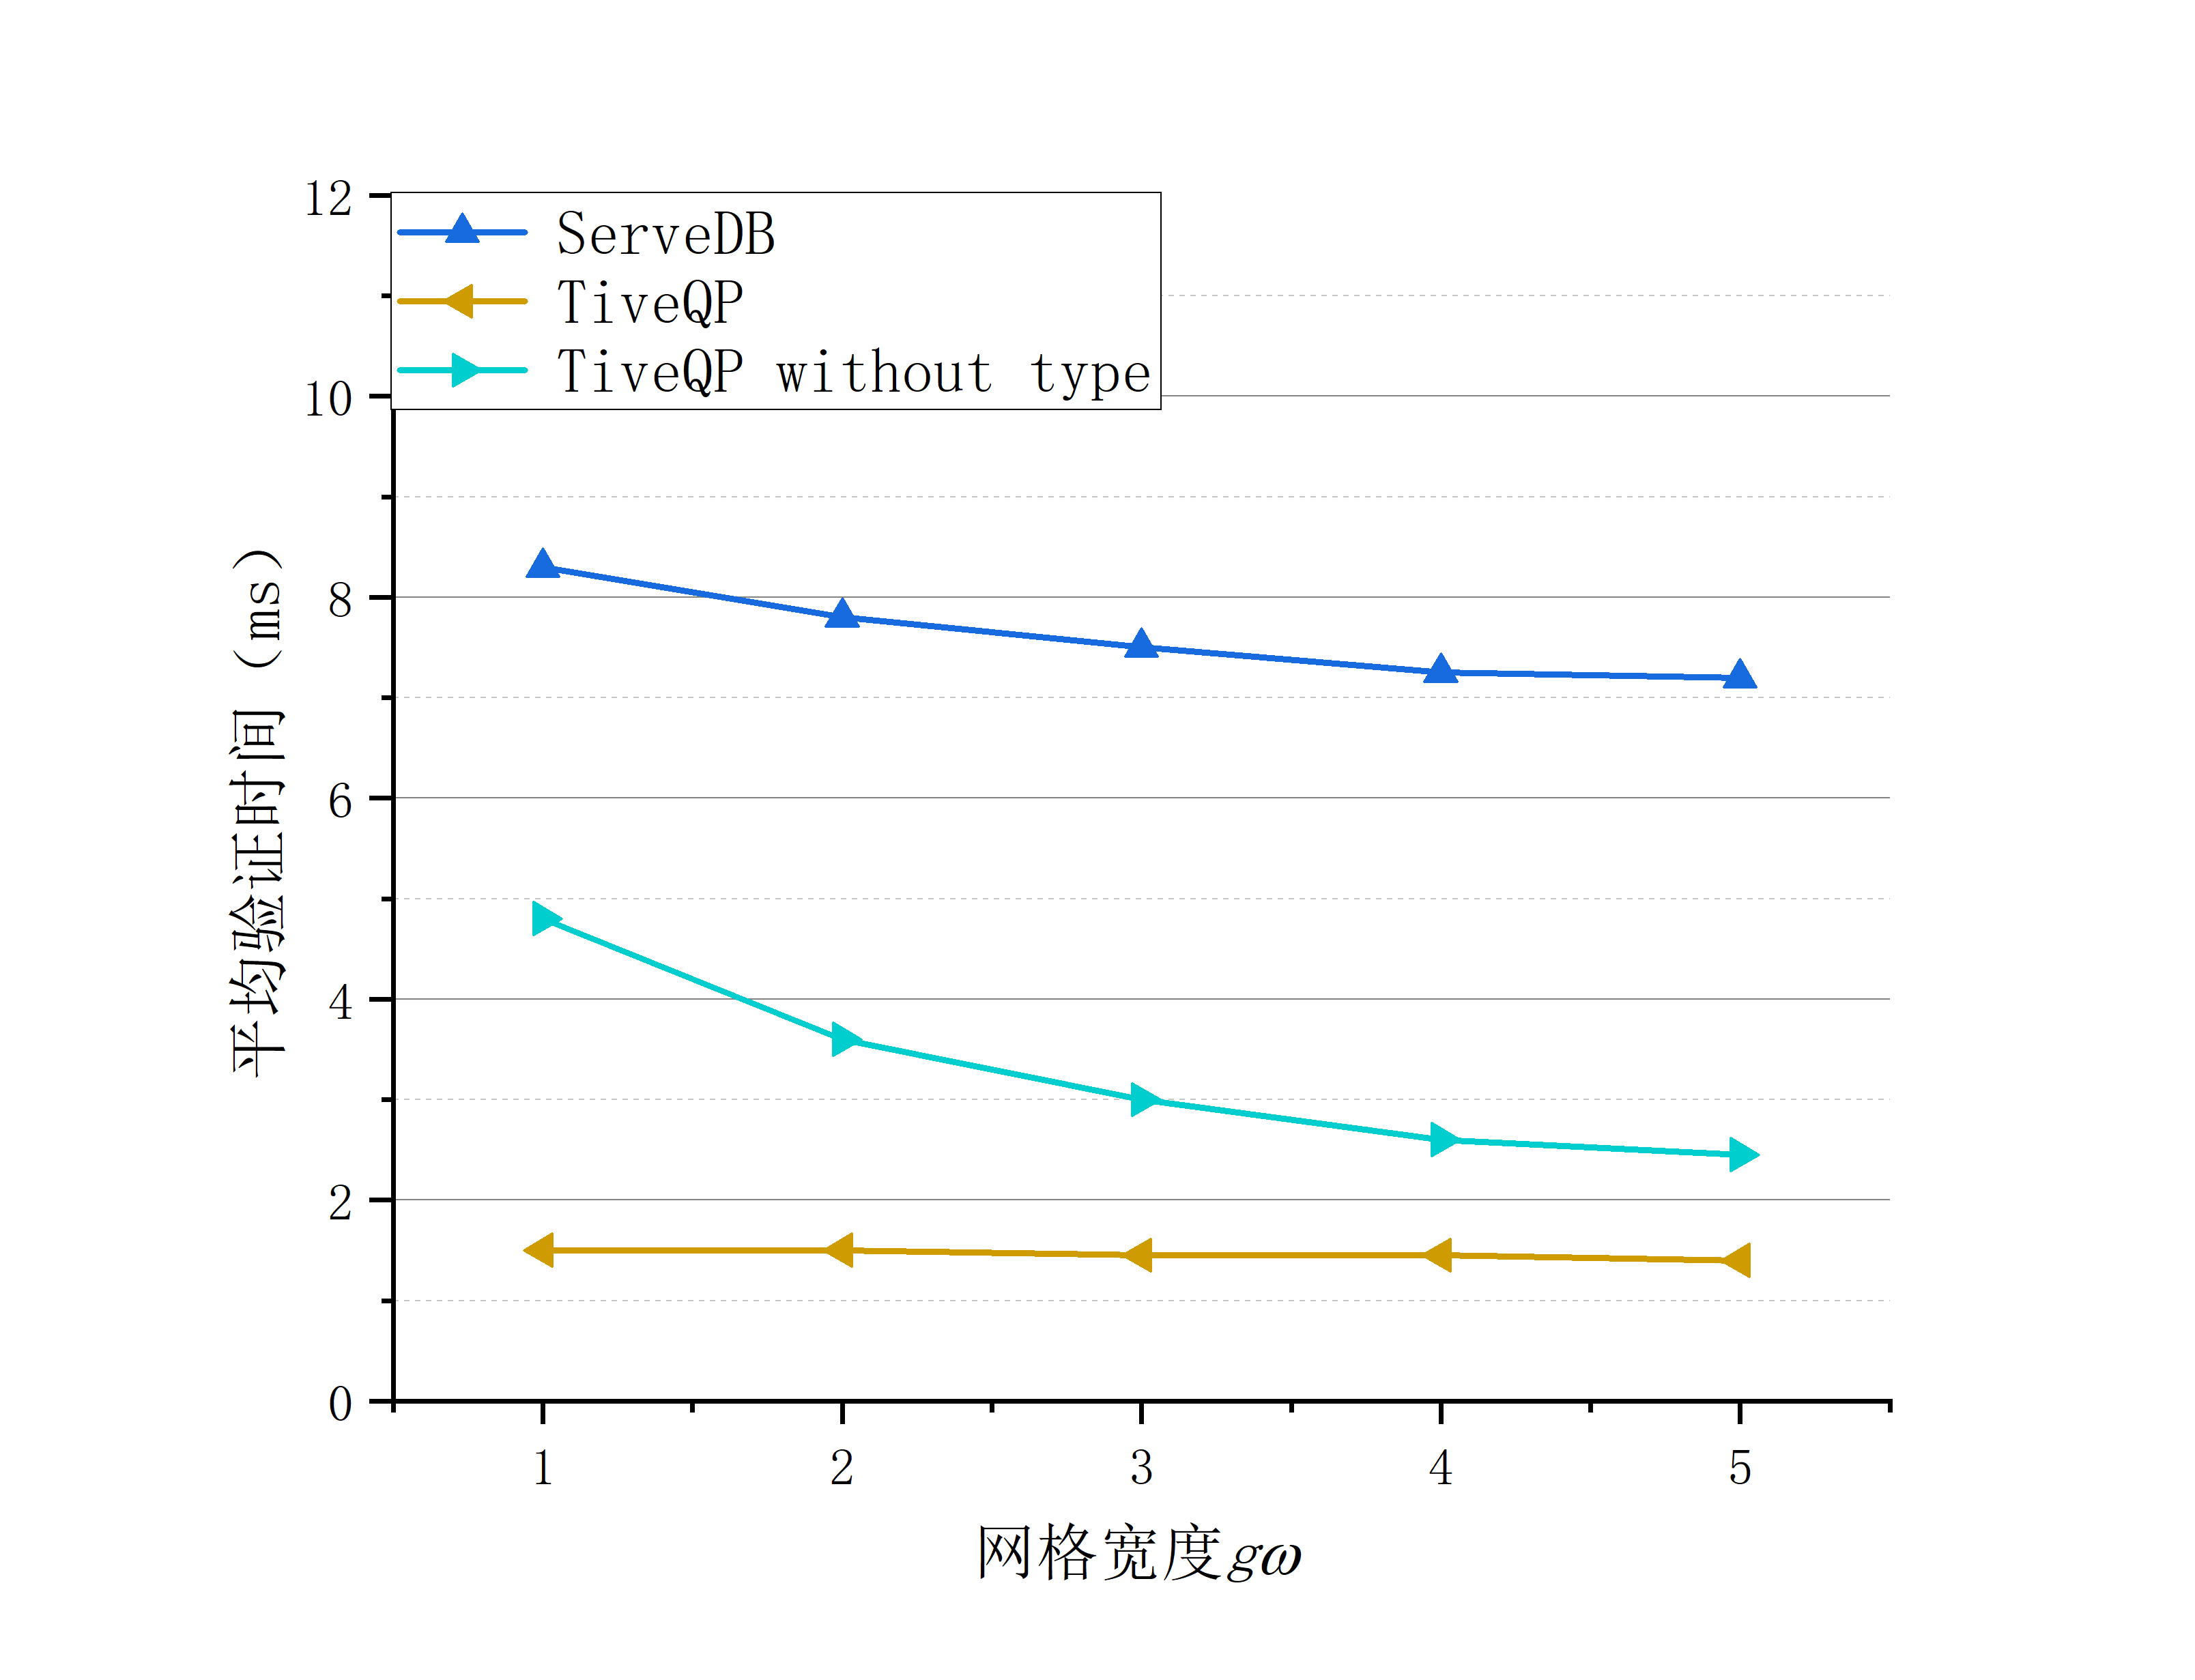
\includegraphics[width=0.3\textwidth]{jpgs/8-b.png}}
    \end{subcaptionbox}
    \hspace{10pt}
    \begin{subcaptionbox}{Average verification time varying \(k\)}
        {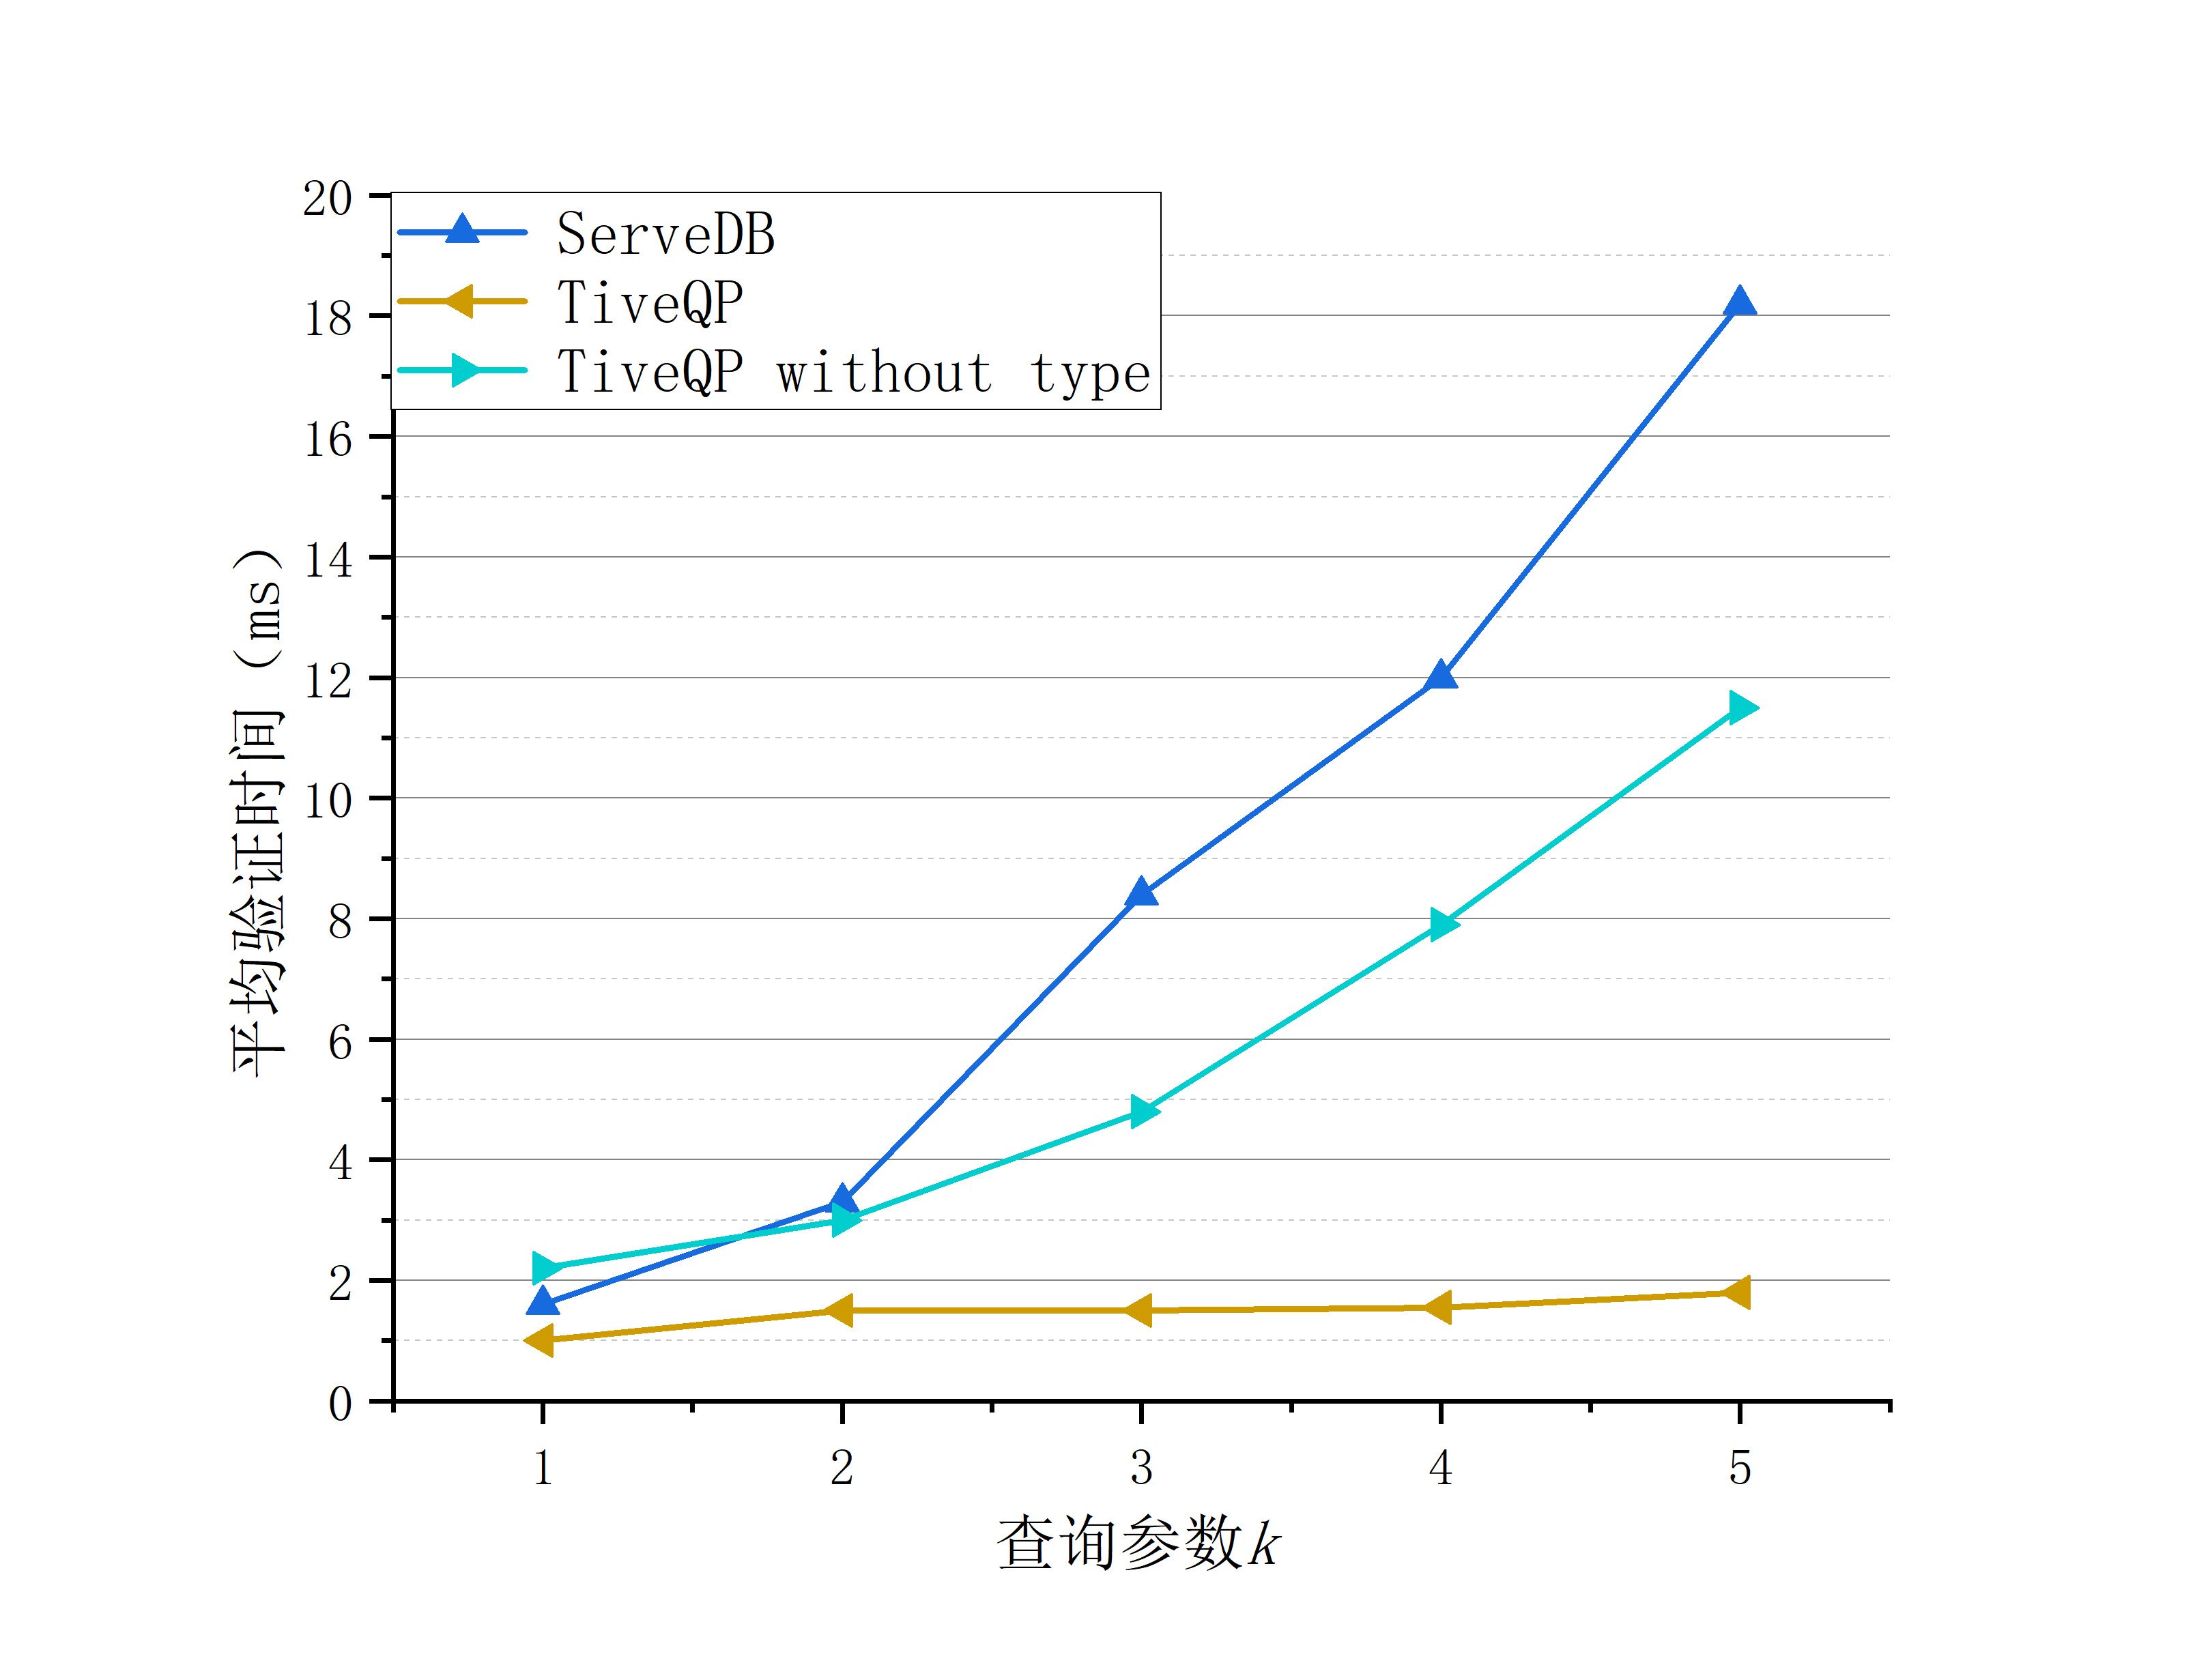
\includegraphics[width=0.3\textwidth]{jpgs/8-c.png}}
    \end{subcaptionbox}
    \caption{平均验证时间随不同参数的变化情况}
    \label{fig:verification_time}
\end{figure}

\subsection{通信代价测试}
图5.4(a)、5.4(b)和5.4(c)分别展示了关于不同的 \(n\)、\(gw\) 和 \(k\) 的通信开销(假设插入相关图片)。通信开销不会随 \(n\) 变化,原因与查询处理中的相同。当 \(gw\) 增加时,网格数量减少,网格编码的大小也随之减小,从而降低了通信开销。

\begin{figure}[h]
    \centering
    \begin{subcaptionbox}{Proof size varying \(n\)}
        {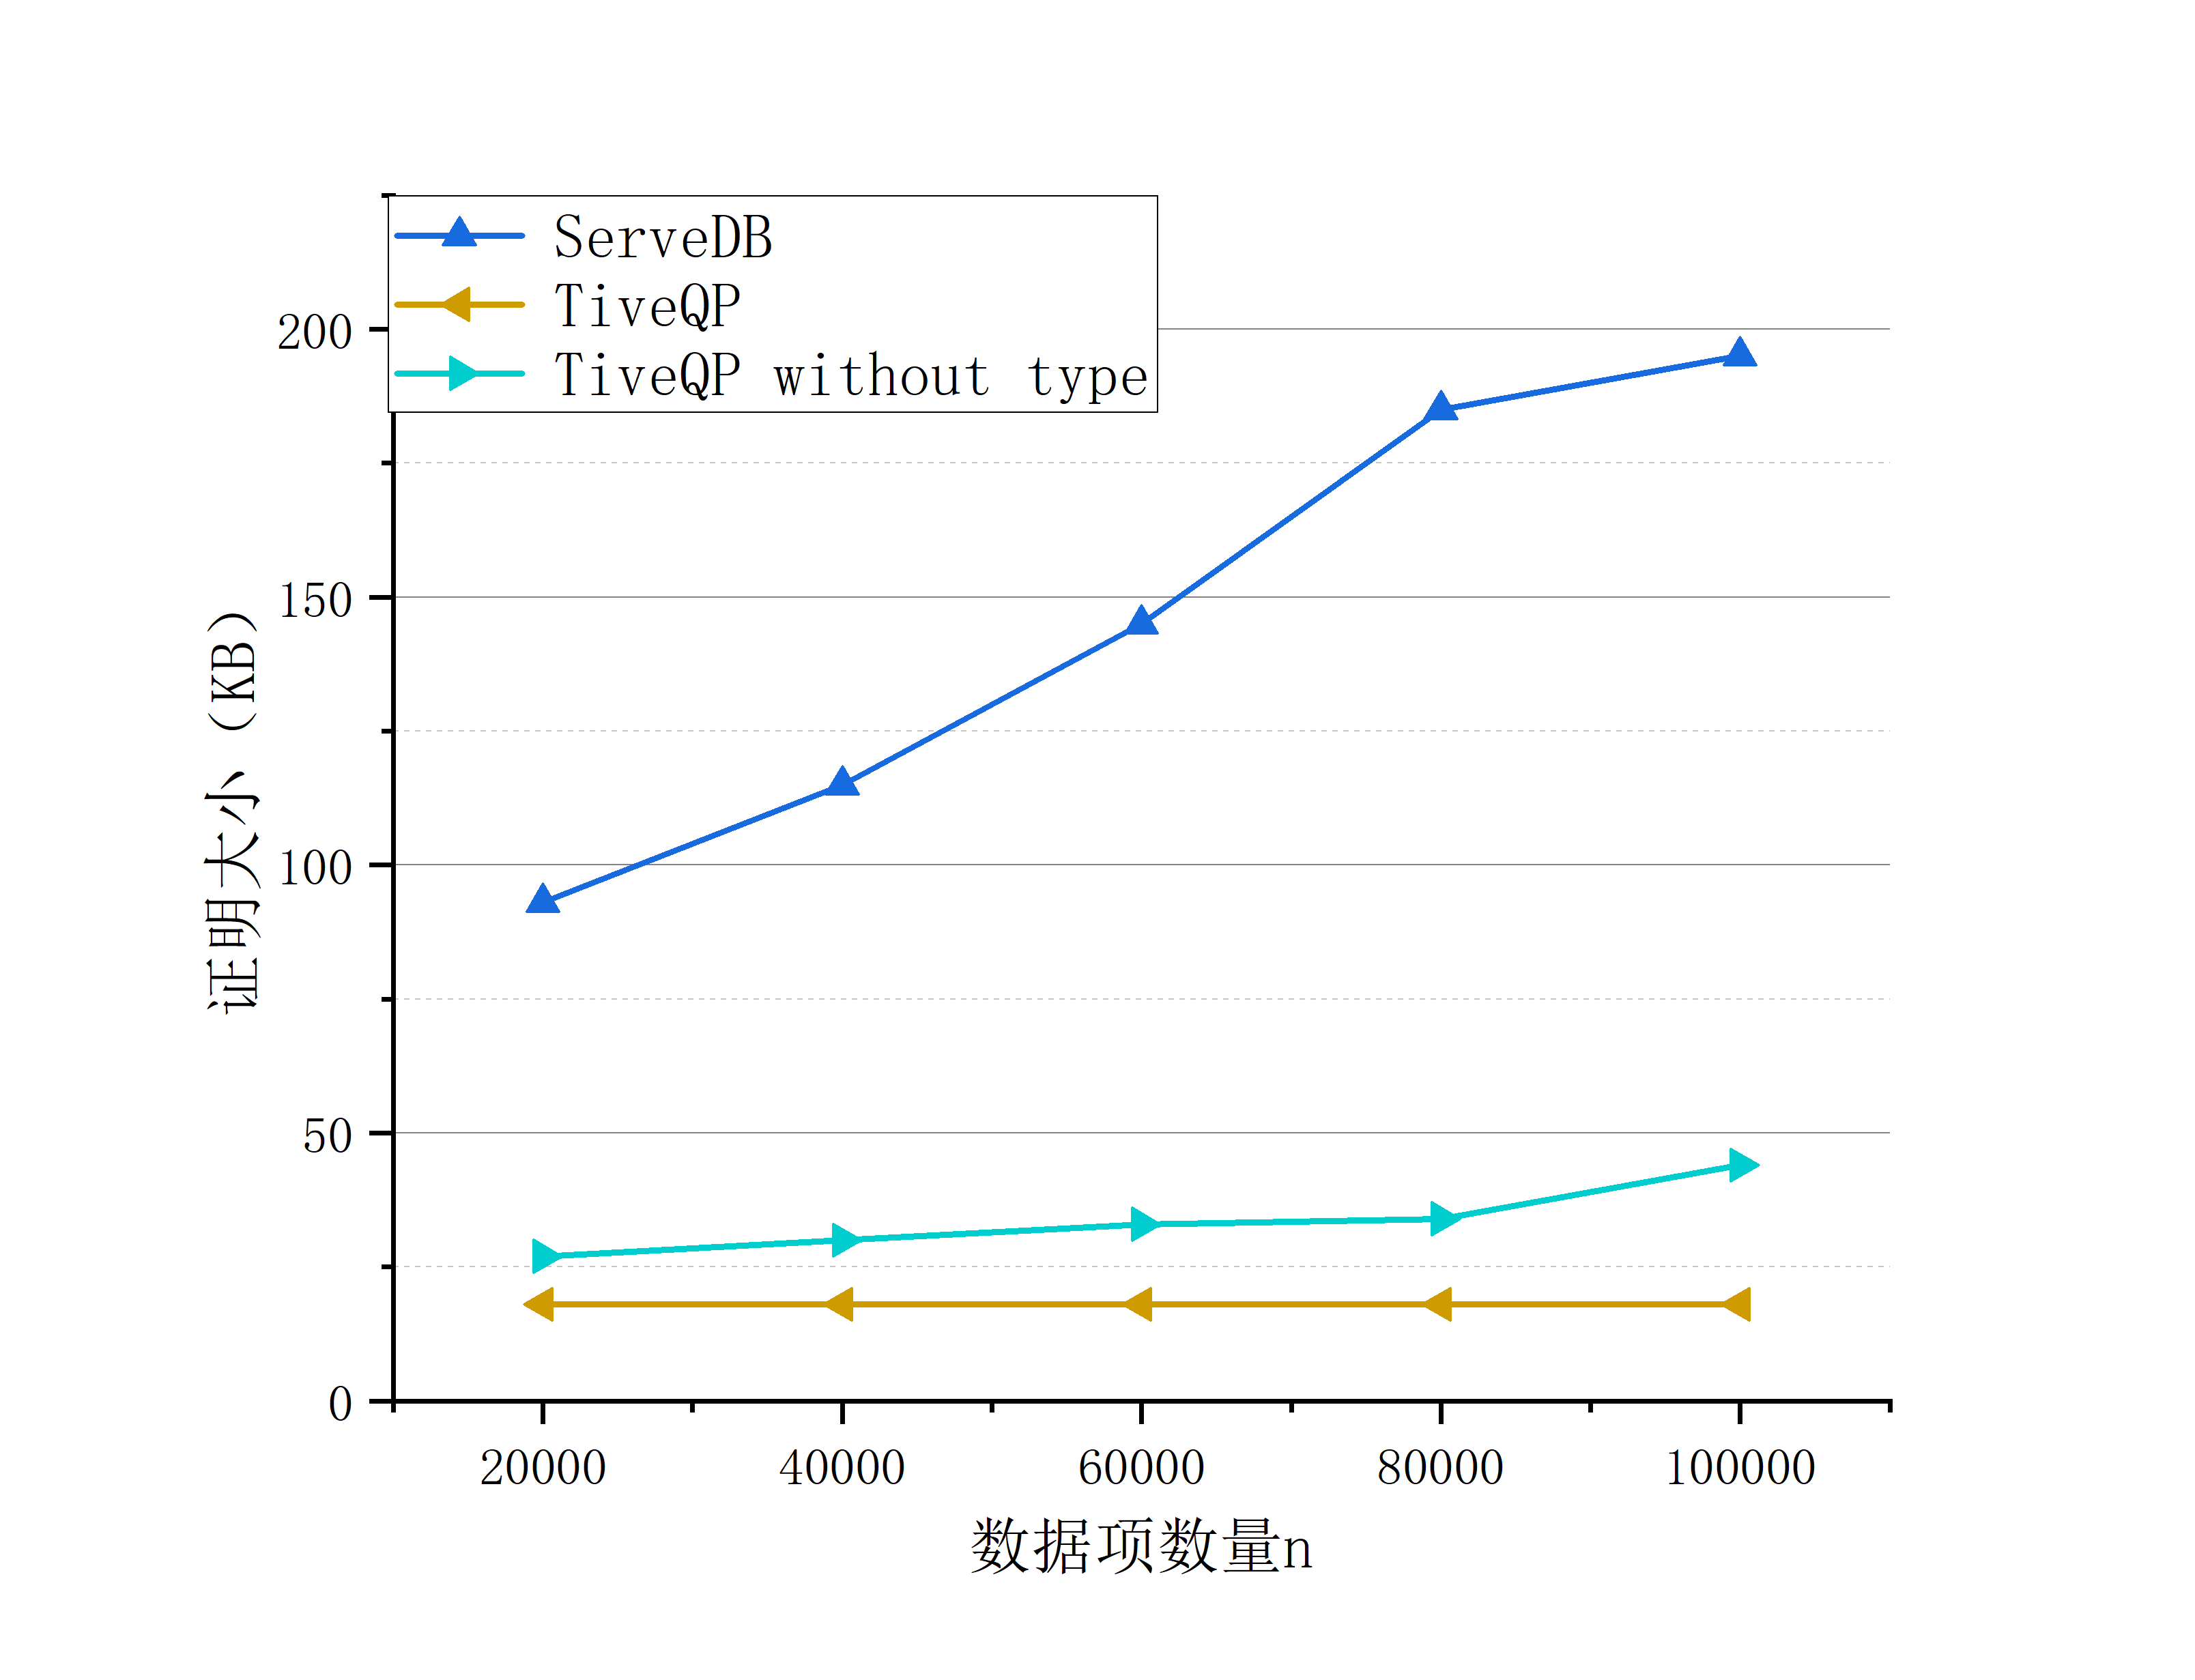
\includegraphics[width=0.3\textwidth]{jpgs/7-d.png}}
    \end{subcaptionbox}
    \hspace{10pt}
    \begin{subcaptionbox}{Proof size varying \(gw\)}
        {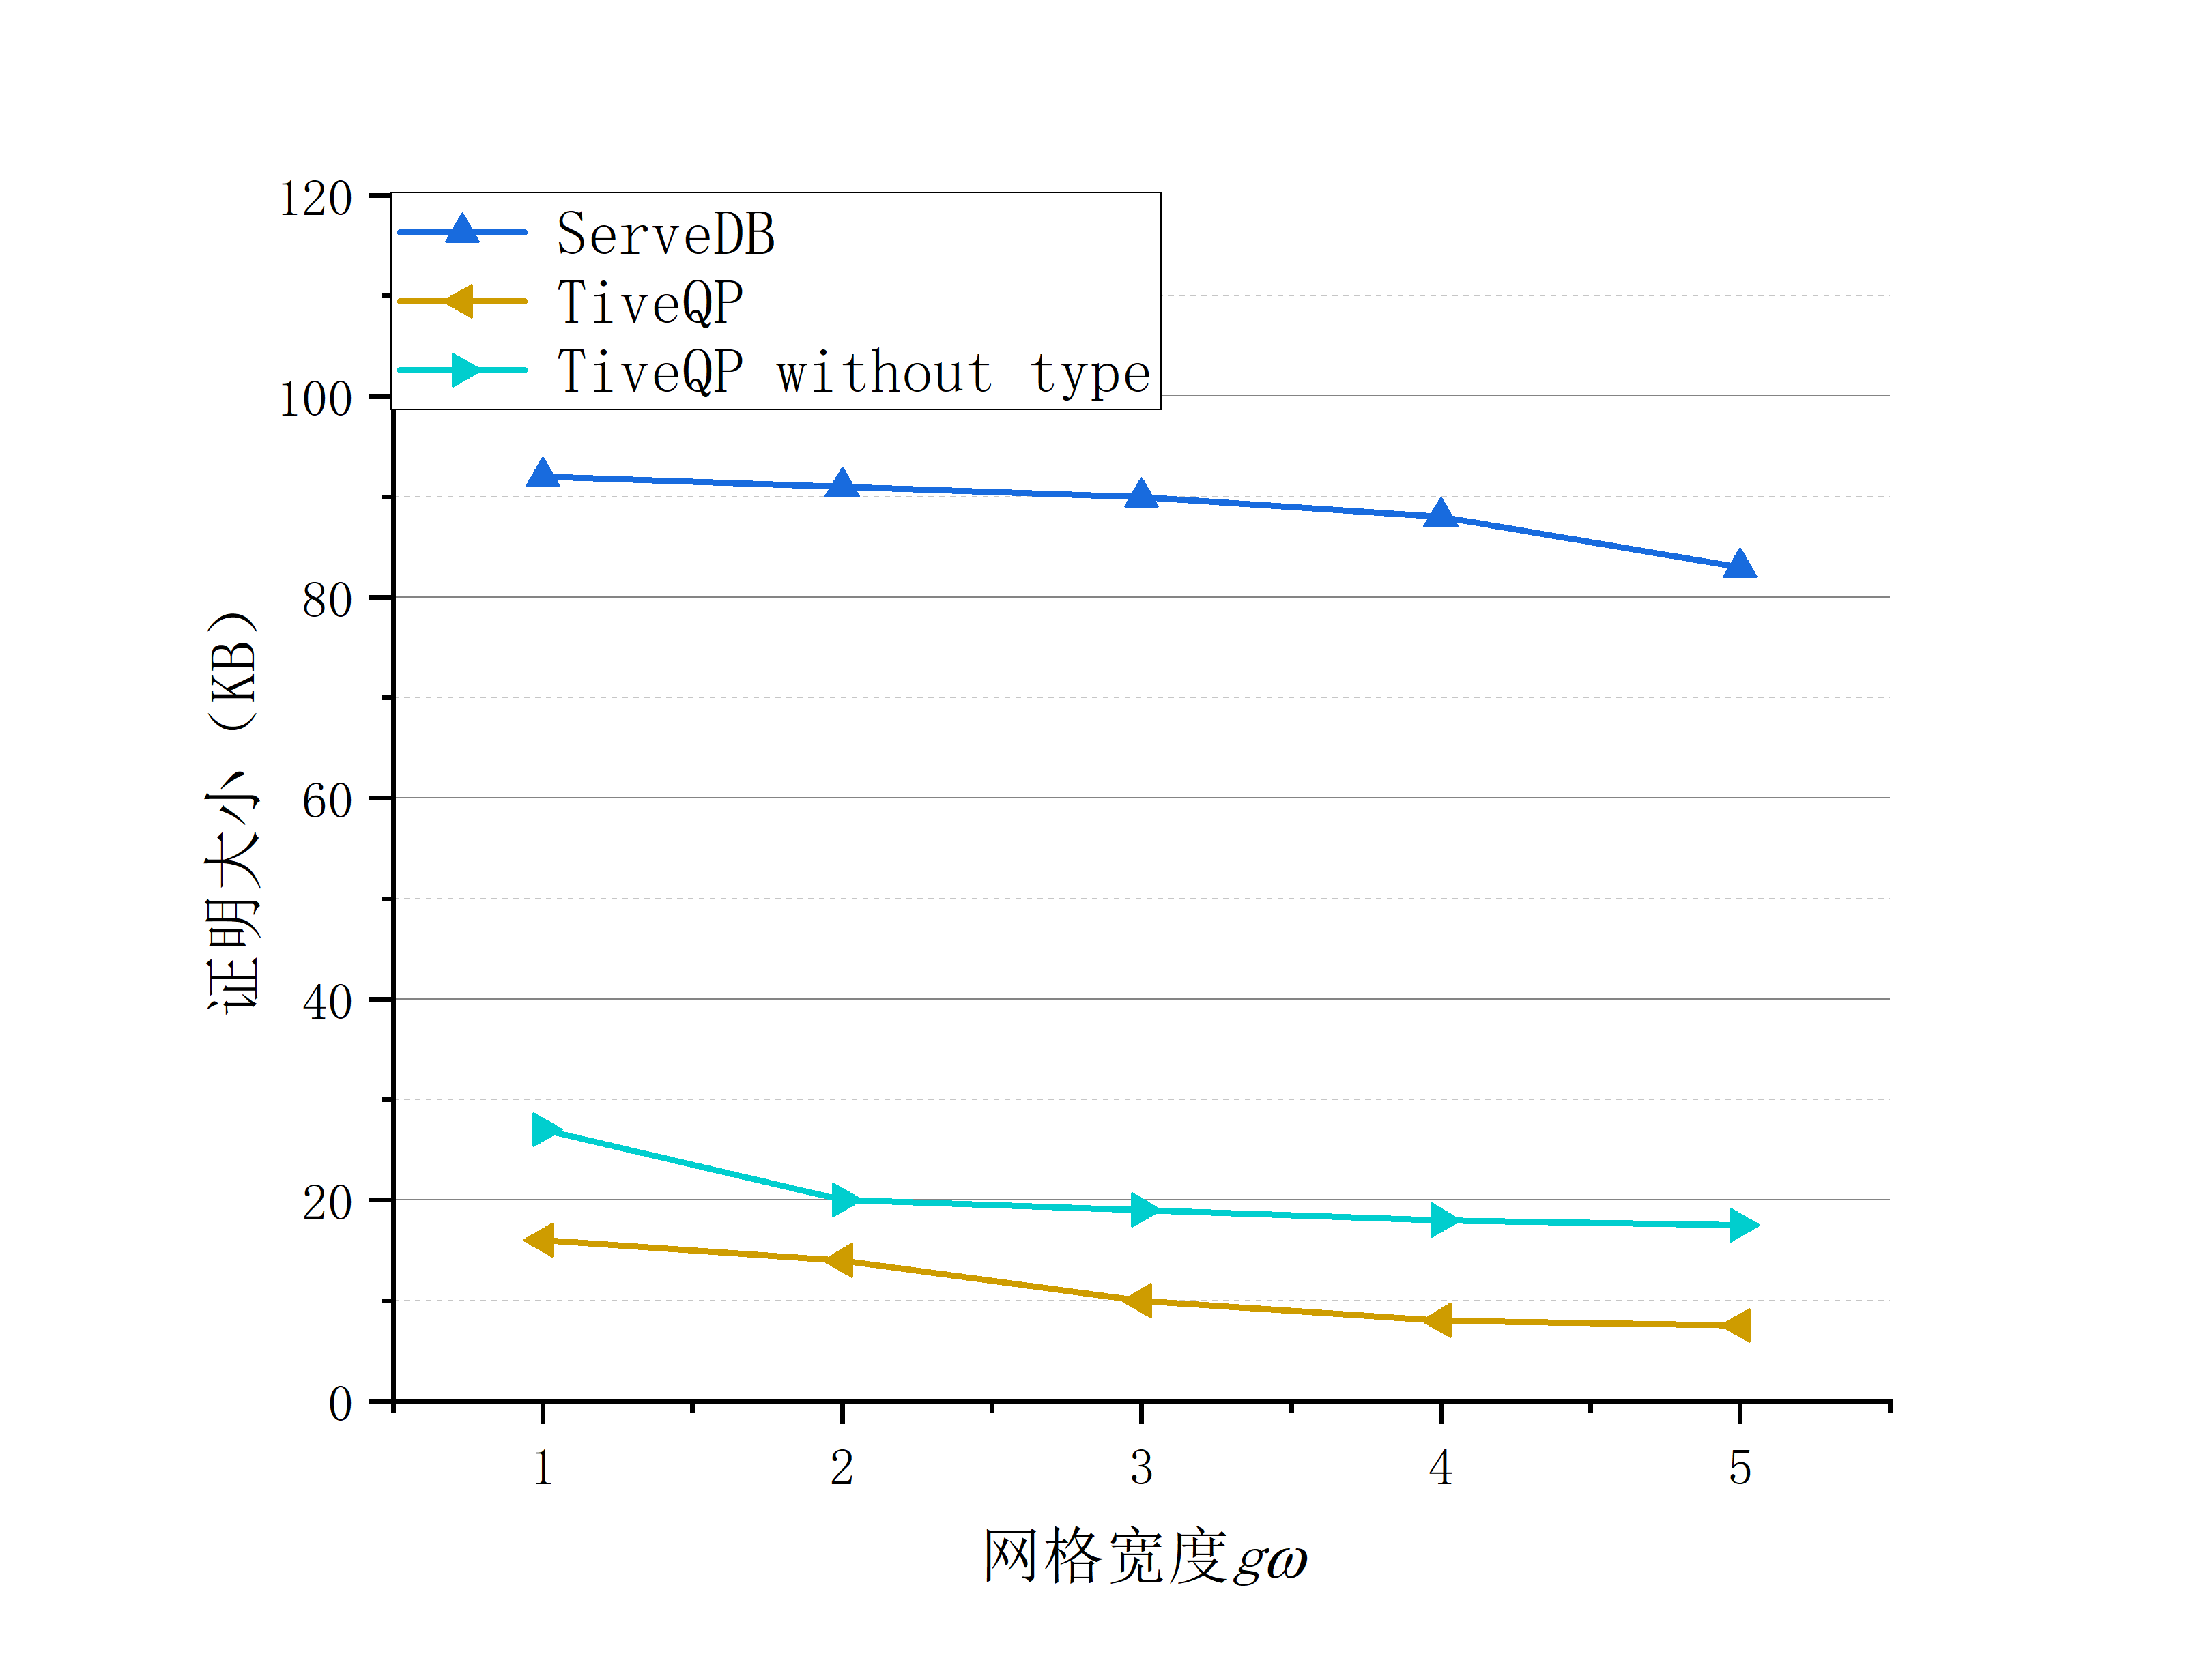
\includegraphics[width=0.3\textwidth]{jpgs/7-e.png}}
    \end{subcaptionbox}
    \hspace{10pt}
    \begin{subcaptionbox}{Proof size varying \(k\)}
        {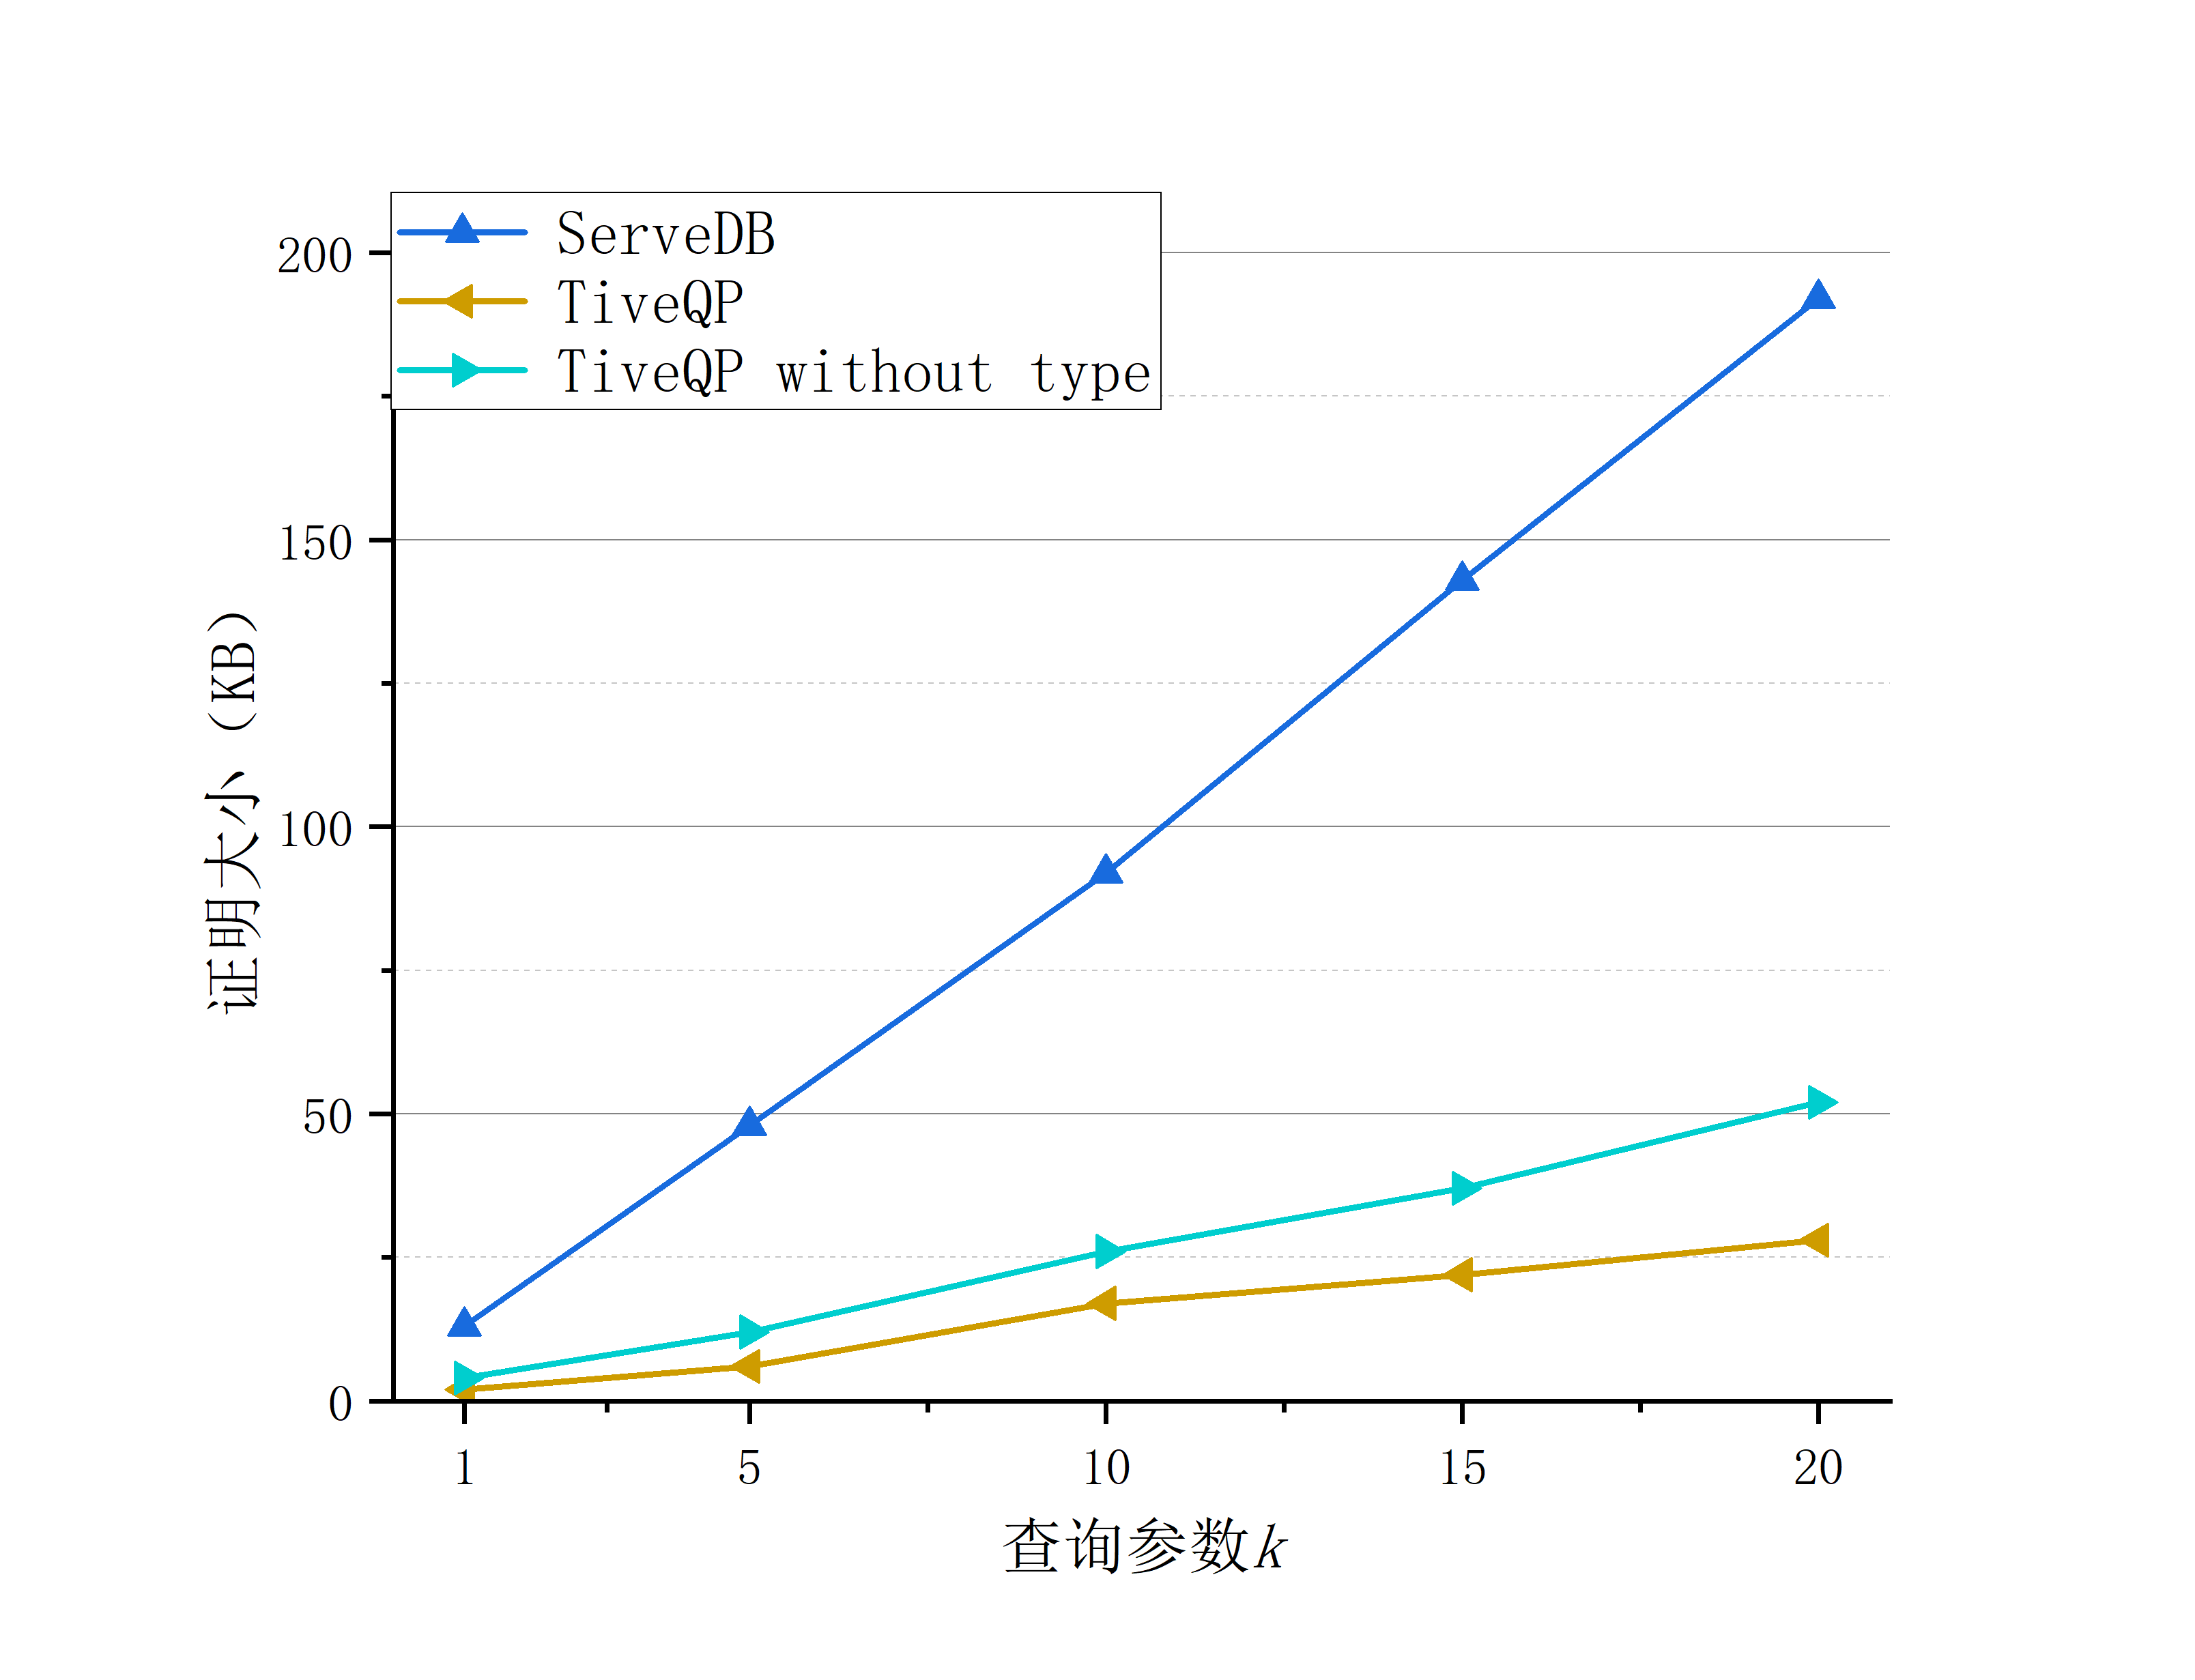
\includegraphics[width=0.3\textwidth]{jpgs/7-f.png}}
    \end{subcaptionbox}
    \caption{证明大小随不同参数的变化情况}
    \label{fig:proof_size}
\end{figure}

\newpage
\section{创新性说明}
TiveQP系统是一款极具创新性的限时、可验证且高效的SkNN查询处理系统。它深度融合了空间编码技术、前缀编码技术、不可区分的布隆过滤器(IBF)、互补集(CS)概念以及剪枝策略等前沿技术,成功打造出安全、高效且能充分保护隐私的查询处理与结果验证机制。该系统的核心创新优势显著,其独特的编码与查询整合方式极大提升了查询效率,同时,借助隐私保护验证方法和精妙的剪枝策略,TiveQP系统不仅确保了查询结果的可验证性,更显著增强了查询过程中数据的隐私保护力度。此外,系统通过严格的理论分析和丰富的实验验证,充分展现了在理论层面的严谨性以及实际应用中的高效性,为云计算环境下的加密数据查询处理提供了极具价值的实践方案。

\subsection{扩展SkNN以支持隐私保护的时间受限访问}
TiveQP系统开创性地对SkNN进行扩展,实现了对隐私保护的时间受限访问。系统运用空间编码技术精准处理位置信息,同时利用前缀编码技术巧妙处理位置和时间信息,并将编码后的结果巧妙插入不可区分的布隆过滤器(IBF)。通过把每个查询精心编码为一个陷门,系统将原本分别针对空间属性和时间属性的处理查询,完美整合为对联合关键字的查询。这种创新方式在有效解决时间限制访问难题的同时,还充分保障了查询效率,使用户能够在特定时间范围内高效获取所需数据,并且全方位保护了数据的隐私性。

\subsection{提出保护隐私的结果验证方案}
TiveQP系统创造性地提出了互补集(CS)概念,并设计出一套先进的保护隐私的结果验证方案。传统验证方式常常存在数据隐私泄露风险,而该系统另辟蹊径,不直接证明一个位置不在A区域,而是证明其位于A的互补区域。具体来说,数据拥有者针对每份数据精准计算位置、类型和打开时间三个互补集,每个集合被转化为前缀的最小集合,由前缀在IBF节点中生成一个比特段。系统进一步计算段的键控哈希消息认证码(HMAC)作为签名。当证明不匹配时,系统仅将匹配到的比特段与HMAC返回给用户,而非整个IBF或比特段,从而最大程度避免了未查询数据隐私的泄露。

\subsection{设计剪枝策略提高查询处理和结果验证效率}
为大幅提升查询处理和结果验证效率,TiveQP系统精心设计了一种剪枝策略。系统首先依据数据项的空间属性(如类型和城市)对其进行科学分类,然后自上而下为每种位置类型构建子树。通过这一策略,系统有效消除了不必要的搜索路径,显著缩短了查询处理时间和结果验证时间。查询复杂度成功降低到 \(O(k\log(\frac{n}{t*c}))\),其中 \(t\) 和 \(c\) 分别代表类型和城市的数量。该策略让TiveQP系统在面对大规模数据集时,能够迅速响应用户的查询需求,极大提升了系统的整体性能。

\subsection{支持动态数据更新与查询优化}
TiveQP系统具备支持动态数据更新的能力,这是其区别于传统查询系统的重要创新点。在实际应用场景中,数据往往是动态变化的,例如实时的位置数据、时间敏感的数据等。TiveQP系统能够高效地处理这些动态更新,而无需重新构建整个查询结构。系统通过设计一种增量式的编码和更新机制,当有新的数据加入或已有数据发生变化时,只需对相关的编码和布隆过滤器进行局部更新。同时,系统还会根据数据的动态变化,自动调整剪枝策略和查询计划,进一步优化查询性能。这种动态适应性使得TiveQP系统在不断变化的数据环境中始终保持高效稳定的查询处理能力。

\subsection{实现跨平台兼容性与分布式查询处理}
TiveQP系统实现了出色的跨平台兼容性,能够在多种操作系统和硬件环境下稳定运行。无论是在传统的服务器集群上,还是在新兴的云计算平台、边缘计算设备上,TiveQP系统都能无缝部署和高效工作。此外,系统还支持分布式查询处理,通过将查询任务合理分配到多个节点上并行执行,充分利用分布式系统的计算资源和存储能力。在分布式环境中,各个节点之间通过高效的通信协议进行数据交互和结果整合,大大提高了查询处理的速度和可扩展性。同时,系统在分布式处理过程中依然能够严格保证数据的隐私性和查询结果的准确性,为大规模、复杂的数据查询场景提供了强大的支持。

\newpage

\section{总结}
本作品提出了一种限时、可验证、高效的SkNN查询处理方案TiveQP。该方案在设计和实现过程中具备两大重要创新点。其一,通过整合空间属性与时间属性,成功把时间限制这一访问特征引入SkNN查询处理,达成了特定时间范围内的数据高效访问。其二,借助互补集中的成员检查,设计出一种独特的隐私保护验证方法。此方法通过验证数据是否处于互补集中,有效避免了未查询数据隐私的泄露,进而增强了系统的安全性与隐私保护能力。

在提升查询效率方面,本作品引入了新颖的空间编码技术和修剪策略。空间编码技术对数据进行精细编码和优化组织,让查询处理更为高效;修剪策略则智能地减少不必要的搜索路径,显著提高了查询速度和结果验证的效率。这些技术创新使TiveQP在面对大规模数据集时,能够迅速响应用户的查询需求。

为确保TiveQP的安全性,本作品开展了严格的理论分析与证明。通过形式化的安全声明,证实了TiveQP能够有效抵御各类潜在的安全威胁,保障用户数据在云环境中的安全性与完整性。实验结果进一步验证了TiveQP的性能优势。与传统方法相比,TiveQP在查询处理速度和结果验证效率上均有显著提升。实验数据表明,在大规模数据集和高并发查询环境下,TiveQP能够维持稳定的高性能表现。

总体而言,TiveQP不仅在理论层面具有创新性和前瞻性,在实际应用中也展现出强大的实用性和高效性。它将时间限制、空间编码和隐私验证有机结合,实现了高效、安全的SkNN查询处理。这一方案拥有广泛的应用前景,尤其适用于需要高效安全数据访问的场景,例如医疗数据管理、金融数据分析等。未来,TiveQP有望为更多领域的数据安全与查询效率提供可靠的解决方案,推动云计算环境下的数据处理技术迈向新高度。
% 我们将DeTAPS方案划分为五个主要阶段,包括密钥初始化(Setup)、签名生成(Sign)、签名合并(Combine)、签名验证(Verify)和签名溯源(Trace)。DeTAPS系统流程如图\ref{系统流程}所示,图中省略了密钥初始化的过程,上半部分展示了签名生成与合并流程,下半部分展示了签名验证与溯源流程。

% \begin{figure}[H]
% 	\centering
% 	\includegraphics[width=1.0\linewidth]{系统流程图.jpg}
% 	\caption{系统流程图}
% 	\label{系统流程}
% \end{figure}




% \begin{figure}[!ht]
% 	\begin{minipage}[t][0.92\textheight][t]{\textwidth}
% 		\begin{framed}
% 			\fontsize{10pt}{12.3pt}\selectfont
% 			\vspace{-0.1cm}
% 			\noindent\underline{$\mathsf{Setup}(1^{\lambda}, n, n_1, n_2, t):$}\\
% 			\vspace{-0.18cm}
% 			%$\mathcal{U}$ is the set of all $n$ signers, $\mathcal{G}$ is set of signer group identifiers\\
% 			$1.\ (pk, \{sk_i\}^{n}_{i=1}) \leftarrow \mathsf{ATS.KeyGen}(1^{\lambda}, n, t)$\ \textcolor{darkgrey}{//$n$: number of signers}\\
% 			\vspace{-0.18cm}
% 			$2.\ r_{pk} \leftarrow \mathcal{R}_{\lambda}$, $\textsf{com}_{pk} \leftarrow \mathsf{COM.Comm}(pk, r_{pk})$\\
% 			\vspace{-0.18cm}
% 			$3.\ (mk, ek, vk, ck) \leftarrow \mathsf{DTPKE.Setup}(1^{\lambda})$\\
% 			\vspace{-0.18cm}
% 			$4.\ (pk^s_j, sk^s_j) \leftarrow \mathsf{SIG.KeyGen}(1^{\lambda}, j)$, $j\in [n_1]$\ \ \ \textcolor{darkgrey}{//Combiner $C_j$'s signing keys}\\
% 			\vspace{-0.18cm}
% 			$5.\ (pk^e_j, sk^e_j) \leftarrow \mathsf{PKE.KeyGen}(1^{\lambda}, j)$, $j\in [n_1]$\ \textcolor{darkgrey}{//Enclave $E_j$'s encryption keys}\\
% 			\vspace{-0.18cm}
% 			$6.\ (usk_o, upk_o, uvk_o) \leftarrow \mathsf{DTPKE.Join}(mk, o)$, $o\in [n_3]$\ \textcolor{darkgrey}{//$n_3$: number of notaries}\\
% 			\vspace{-0.18cm}
% 			$7.\ (\mathcal{B}, \mathcal{PK}, H) \leftarrow \mathsf{KASE.Setup}(\lambda, |G|)$\\
% 			\vspace{-0.18cm}
% 			$8.\ (mpk, msk) \leftarrow \mathsf{KASE.KeyGen}(\lambda)$\\
% 			\vspace{-0.18cm}
% 			$9.\ k_a \leftarrow \mathsf{KASE.Extract}(msk, \mathcal{G})$\ 
% 			\textcolor{darkgrey}{//$\mathcal{G}$: set of signer groups}\\
% 			\vspace{-0.18cm}
% 			$10.\ sk_j^c \leftarrow (\tikzmark{id}{\colorbox{grey}{$pk, sk^e_j, t, ek, r_{pk}$}}), \tikzmark{kd}j \in [n_1]$\ \textcolor{darkgrey}{//Combining key}\\
% 			\begin{tikzpicture}[overlay, remember picture,node distance =1.0cm]
% 				\node [darkgrey](cd) [above right=of kd ]{\textbf{\underline{stored in Enclave $E_j$}}};
% 				\draw[darkgrey,->,thick] (cd) to [in=10,out=-175] (id);
% 			\end{tikzpicture}
% 			\vspace{-0.08cm}
% 			$11.\ sk_j^t \leftarrow ($\colorbox{grey}{$sk^e_j, ck, pk$}), $j\in [n_2]$\ \ \ \ \ \ \ \ \ \ \ \ \textcolor{darkgrey}{//Tracing key}\\
% 			\vspace{-0.18cm}
% 			$12.\ gid \leftarrow \mathsf{HASH}(GID, time)$, $GID\in \mathcal{G}$\ \ \ 
% 			\textcolor{darkgrey}{//$gid$: signer group identifier}\\
% 			\vspace{-0.18cm}
% 			$13.\ PK \leftarrow (\textsf{com}_{pk}, ek, vk, \{pk^s_i\}^{n_j}_{j=1}, \{pk^e_j\}^{n_1}_{j=1}, \mathcal{B}, \mathcal{PK}, H, mpk, \{gid\})$\\
% 			\vspace{-0.18cm}
% 			$14.$ Output $(PK, \{sk_i\}^{n}_{i=1}, \{sk^s_j\}^{n_1}_{j=1}, \{sk^c_j\}^{n_1}_{j=1}, \{sk^t_j\}^{n_2}_{j=1}, \mathcal{G}, k_a)$\\
% 			\vspace{-0.1cm}
% 			\underline{$\mathsf{Sign}(sk_i, m, \mathcal{S}, \mathcal{N}) \rightarrow \widehat{\sigma_i}:$}\\
% 			\vspace{-0.18cm}
% 			$1.\ \sigma_i\leftarrow \textsf{ATS.Sign}(sk_i, m, \mathcal{S})$\\
% 			\vspace{-0.18cm}
% 			$2.\ \widehat{\sigma}_i\leftarrow \mathsf{PKE.Enc}(pk^e_j, m||\sigma_i||\mathcal{N}||gid)$\ %\textcolor{darkgrey}{//Sent to CB to be processed by a combiner}\\
			
% 			\vspace{-0.05cm}
% 			\noindent\underline{$\mathsf{Combine}(\colorbox{grey}{$sk^c_j=(pk, sk^e_j, t, ek, r_{pk}$)}, sk^s_j, m, \mathcal{S}, \{\widehat{\sigma_i}\}_{i\in \mathcal{S}})\rightarrow \sigma$}\\
% 			\vspace{-0.1cm}
% 			\colorbox{grey}{
% 				$1.\ (m||\sigma_i||\mathcal{N}||gid)\leftarrow \mathsf{PKE.Dec}(\widehat{\sigma}_i, sk^e_j)$\ \textcolor{darkgrey}{//\textbf{Enter $E_i$} here; $\sigma_i\in$ Tx pool}}\\
% 			\vspace{-0.18cm}
% 			\colorbox{grey}{
% 				$2.\ \sigma^m \leftarrow \mathsf{ATS.Combine}(pk, m, \mathcal{S}, \{\sigma_i\}_{i\in \mathcal{S}})$}\\
% 			\vspace{-0.18cm}
% 			\colorbox{grey}{
% 				$3.\ \overline{\sigma}\leftarrow \mathsf{DTPKE.Enc}(ek, \mathcal{N}, \sigma^m)$}\\
% 			\vspace{-0.18cm}
% 			\colorbox{grey}{
% 				$4.\ (c^{gid}_1, c^{gid}_2, \{ind_o\}_{o\in \mathcal{N}})\leftarrow \mathsf{KASE.Enc}(mpk, gid, \mathcal{N})$}\\
% 			\vspace{-0.18cm}
% 			\colorbox{grey}{
% 				5. Generate a proof for the relation:}
% 			\vspace{-0.4cm}
% 			\begin{equation*}
% 				\mathcal{R}((t', \textsf{com}_{pk}, ek, mpk, m, \overline{\sigma}, gid, c^{gid}_1, c^{gid}_2, \{ind_o\}_{o\in \mathcal{N}}); (\mathcal{N}, \sigma^m, r_{pk}, pk)) = \textrm{1 iff}
% 				\vspace{-0.3cm}
% 			\end{equation*}
% 			\begin{equation*}
% 				\left\{
% 				\begin{aligned}
% 					&\mathcal{N} \subseteq [n_3],\ \mathsf{ATS.Verify}(pk, m, \sigma^m) = 1,\ \mathsf{COM.Verify}(pk, r_{pk}, \textsf{com}_{pk}) = 1,\\
% 					&\overline{\sigma} = \mathsf{DTPKE.Enc}(ek, \mathcal{N}, \sigma^m),\ (c_1, c_2, \{ind_o\}_{o\in \mathcal{N}})\leftarrow \mathsf{KASE.Enc}(mpk, gid, \mathcal{N}).\\
% 				\end{aligned}
% 				\right\}
% 			\end{equation*}
% 			\vspace{-0.18cm}
% 			$6.\ \eta\leftarrow \mathsf{SIG.Sign}(sk^s_j, (m, \overline{\sigma}, c^{gid}_1, c^{gid}_2, \{ind_o\}_{o\in \mathcal{N}}, \pi))$\\
% 			\vspace{-0.18cm}
% 			$7.$ Output a DeTAPS signature $\sigma\leftarrow (\overline{\sigma}, c^{gid}_1, c^{gid}_2, \{ind_o\}_{o\in \mathcal{N}}, \pi, \eta)$\\
% 			\vspace{-0.1cm}
% 			\underline{$\mathsf{Verify}(PK, m, \sigma)\rightarrow\ \{0,1\}$}\\
% 			\vspace{-0.18cm}
% 			1. Accept $\sigma$ if $\mathsf{SIG.Verify}(pk^s_j, m, \sigma) = 1$ and $\pi$ is valid; reject otherwise.\\
% 			\vspace{-0.02cm}
% 			\underline{$\mathsf{Trace}(sk^t_j = (\colorbox{grey}{$sk^e_j, ck, pk$}), m, \sigma) \rightarrow \mathcal{S}$}\\
% 			\vspace{-0.15cm}
% 			$1.\ td_o \leftarrow \mathsf{KASE.Trapdoor}(k_a, pid_o)$\ \textcolor{darkgrey}{//For each notary with a pseudo identity $pid_o$}\\
% 			\vspace{-0.18cm}
% 			$2.\ td^{gid}_o\leftarrow \mathsf{KASE.Adjust}(\mathcal{B}, \mathcal{PK}, H, gid, \mathcal{G}, td_o)$\ \textcolor{darkgrey}{//For each $gid$ and $td_o$}\\
% 			\vspace{-0.18cm}
% 			$3.\ \{0,1\}\leftarrow \mathsf{KASE.Test}(td^{gid}_o, (c^{gid}_1, c^{gid}_2, \{ind_o\}))$\ \textcolor{darkgrey}{//Search all indexes to locate $\overline{\sigma}$}\\
% 			\vspace{-0.18cm}
% 			4. If $\mathsf{SIG.Verify}(pk^s_j, (m, \overline{\sigma}, \pi), \eta) \neq 1$, output fail and return.\\
% 			\vspace{-0.18cm}
% 			5. $\delta_o \leftarrow \mathsf{DTPKE.ShareDecrypt}(pid_o, usk_o, \overline{\sigma})$\ \textcolor{darkgrey}{//For each $pid_o$ and each $m$}\\
% 			\vspace{-0.18cm}
% 			6. $\overline{\delta}_o\leftarrow \mathsf{PKE.Enc}(pid_o, uvk_o, \delta_o, pk^e_j)$\\
% 			\vspace{-0.1cm}
% 			\colorbox{grey}{
% 				7. $(pid_o, uvk_o, \sigma^m_o) \leftarrow \mathsf{PKE.Dec}(\overline{\delta}_o, sk^e_j)$}\\
% 			\vspace{-0.18cm}
% 			\colorbox{grey}{
% 				8. $\{0,1\}\leftarrow \mathsf{DTPKE.ValidateCT}(ek, \mathcal{N}, \overline{\sigma})$}\ \textcolor{darkgrey}{//Assume that $\overline{\sigma}$ is preloaded}\\
% 			\vspace{-0.15cm}
% 			\colorbox{grey}{
% 				9. $\{0, 1\}\leftarrow \mathsf{DTPKE.ShareVerify}(vk, pid_o, uvk_o, \overline{\sigma}, \delta_o)$}\\
% 			\vspace{-0.15cm}
% 			\colorbox{grey}{
% 				10. $\sigma^m\leftarrow \mathsf{DTPKE.Combine}(ck, \mathcal{N}, \overline{\sigma}, \{\delta_o\}_{o\in \mathcal{N}})$}\\
% 			\vspace{-0.18cm}
% 			\colorbox{grey}{
% 				11. $\mathcal{S}\leftarrow \mathsf{ATS.Trace}(pk, m, \sigma^m)$.}
% 			\vspace{-0.1cm}
% 		\end{framed}
% 	\end{minipage} 
% 	\caption{DeTAPS方案}
% 	\label{DeTAPS}
% \end{figure}

% \setlength{\parindent}{2em}

% \textbf{(1) $\mathsf{Setup}(1^{\lambda}, n, n_1, n_2, t):$ } 
% 在初始化阶段,系统为所有参与者生成所需的密钥,包括为$n$个签名者生成各自的私钥$sk_i$,为$n_1$个合并者生成合并密钥$sk_c$,以及为$n_2$个溯源者生成溯源密钥$sk_t$。
% 同时,生成一个公钥$pk$和相关的加密密钥、解密密钥等,用于后续的签名合并和溯源过程。
% \textbf{\bfseries\siyuan{此外,还确定了一组公证人$\mathcal{N}$,他们负责在签名溯源阶段参与解密和验证过程。}}

% \textbf{(2) $\mathsf{Sign}(sk_i, m, \mathcal{S}, \mathcal{N}) \rightarrow \widehat{\sigma_i}:$}
% 签名者利用其私钥对消息$m$进行签名,生成签名份额$\sigma_i$。
% 签名者将签名份额加密后发送到区块链,以便后续由合并者进行处理。

% \textbf{(3) $\mathsf{Combine}(sk^c_j=(pk, sk^e_j, t, ek, r_{pk}), sk^s_j, m, \mathcal{S}, \{\widehat{\sigma_i}\}_{i\in \mathcal{S}})\rightarrow \sigma:$}
% 不可信的合并者被选举出来,从区块链上收集$t$个签名份额。
% 合并者在TEE内部执行合并任务,对收集到的签名份额进行解密,并生成一个完整的门限签名$\sigma$。
% 在TEE外部,合并者还会生成一个加密的门限签名,并创建一个非交互式零知识证明,证明签名的有效性而无需泄露任何敏感信息。

% \textbf{(4) $\mathsf{Verify}(PK, m, \sigma)\rightarrow\ \{0,1\}:$}
% 任何节点都可以使用公钥$pk$验证生成的门限签名$σ$是否有效,此过程在TEE外部执行。如果有效,输出1;如果无效,输出0。

% \textbf{(5) $\mathsf{Trace}(sk^t_j = (sk^e_j, ck, pk), m, \sigma) \rightarrow \mathcal{S}:$}
% 当需要溯源签名到具体的签名者时,系统唤醒一组公证人$\mathcal{N}$。
% 公证人使用他们的聚合密钥和伪身份生成陷门$td$,并在智能合约的帮助下搜索匹配的索引。
% 如果匹配成功,公证人将部分解密门限签名,并将其发送给请求者。
% 溯源者使用溯源密钥$sk_t$在TEE内部对部分解密的份额进行进一步处理,以溯源到原始的签名者集合。

% 我们的DeTAPS方案如图\ref{DeTAPS}所示。

% \subsection{系统架构}

% 本节将从功能与软件两个方面阐述DeTAPS系统的架构。

% \subsubsection{功能架构}

% \textbf{(1)\bfseries\siyuan{单点认证模块}}

% 为了保障用户的数据安全和实现系统的权限控制,本系统应用单点登录和JWT令牌实现用户登录认证。用户只需要选择自己的身份,使用账号密码登录客户端,其余过程将交给客户端登录与认证模块完成。客户端单点登录模块流程如图\ref{单点认证登录}所示。

% \begin{figure}[H]
% 	\centering
% 	\includegraphics[width=0.7\linewidth]{单点认证登录.pdf}
% 	\caption{单点认证登录}
% 	\label{单点认证登录}
% \end{figure}

% \textbf{(2)\bfseries\siyuan{签名模块}}

% 签名模块在DeTAPS系统中扮演着核心角色。当用户通过客户端提交需要签名的消息$m$时,他们必须选择参与签名的签名者身份。系统在这一步骤中记录下用户的身份标识$gid$。随后,每个签名者利用他们各自的私钥$sk_i$生成对应的签名份额$\sigma_i$。这个签名份额随后被加密,使用的是Enclave中存储的Combiner的公钥$pk$,以确保在传输过程中的安全性。签名份额通过区块链网络发送,等待足够的签名份额收集以进行下一步的合并过程。签名模块示意图如图\ref{签名模块示意图}所示。

% \begin{figure}[H]
% 	\centering
% 	\includegraphics[width=0.6\linewidth]{签名模块.pdf}
% 	\caption{签名模块示意图}
% 	\label{签名模块示意图}
% \end{figure}

% \textbf{(3)\bfseries\siyuan{合并模块}}

% 一旦收集到足够的签名份额,合并模块便开始工作。合并者负责收集所有通过区块链网络发送来的签名份额。他们首先使用自己的私钥对每个签名份额进行解密,恢复出原始的签名份额。随后,在Enclave提供的安全环境中,合并者利用合并密钥$sk_c$​
% 将这些签名份额合并成一个完整的签名$\sigma^m$。为了增强安全性和隐私保护,合并者进一步采用动态门限公钥加密(DTPKE)对完整签名$\sigma^m$进行加密,生成一个加密的门限签名$\overline{\sigma}$。此外,为了向外界证明签名的有效性而不泄露任何额外信息,合并者还生成了一个零知识证明。合并模块示意图如图\ref{合并模块示意图}所示。

% \begin{figure}[t]
% 	\centering
% 	\includegraphics[width=0.9\linewidth]{Combiner_sgx2.jpg}
% 	\caption{合并模块示意图}
% 	\label{合并模块示意图}
% \end{figure}

% \textbf{(4)\bfseries\siyuan{公证模块}}

% 公证模块进一步提升了签名的合法性和透明度。在签名过程中,签名者能够从 $n$ 个公证人中根据具体需求动态设定门限 $t'$。每个公证人有一个伪身份$pid$。在公证过程中,需要至少 $t'$ 个公证人合作来完成溯源任务。在溯源时,这些公证人利用聚合密钥来生成用于识别签名的陷门。接着,公证人会对每一个签名应用调整算法来获得调整后的陷门,随后使用定位算法来定位到与待溯源的签名组相关的签名。合并者在生成零知识证明的同时,计算一个与公证人集合$\mathcal{N}$相关的索引$ind$,并利用密钥聚合可搜索加密(KASE)生成与$ind$相关联的加密信息。这一步骤确保了只有在足够数量的公证人同意的情况下,签名才能被进一步解密和验证。公证模块示意图如图\ref{公证模块示意图}所示。

% \begin{figure}[H]
% 	\centering
% 	\includegraphics[width=0.8\linewidth]{公证模块.pdf}
% 	\caption{公证模块示意图}
% 	\label{公证模块示意图}
% \end{figure}

% \textbf{(5)\bfseries\siyuan{溯源模块}}

% 溯源模块为系统提供了溯源签名来源的能力。当需要溯源一个签名时,将唤醒选定的公证人,他们使用各自的伪身份$pid_i$和陷门$td_i$通过KASE定位到与其相关的签名,然后解密加密后的门限签名$\overline{\sigma}$,然后上传到区块链。溯源者收集到至少$t'$个公证人的解密份额后,在Enclave中结合这些份额对$\overline{\sigma}$进行解密,进而通过签名验证算法确认签名的有效性,并溯源到原始的签名者集合。这一流程不仅保障了签名的不可抵赖性,同时也限制了溯源操作只能在必要时由授权的实体执行。溯源模块示意图如图\ref{溯源模块示意图}所示。

% \begin{figure}[H]
% 	\centering
% 	\includegraphics[width=0.9\linewidth]{Tracer_sgx2.jpg}
% 	\caption{溯源模块示意图}
% 	\label{溯源模块示意图}
% \end{figure}

% \textbf{(6)\bfseries\siyuan{区块链模块}}

% 区块链作为一个不可篡改的分布式账本,记录了所有签名者、合并者、公证人和溯源者的交易和行为日志,确保了系统的透明性和可审计性。每个签名份额在被签名者加密后,作为交易的一部分被提交到区块链上,由网络节点验证并打包进区块中。智能合约部署在区块链上,自动执行包括合并者的选举、公证人的选取、签名份额的收集与验证、以及签名的验证和溯源等过程。共识机制确保了网络中的节点就交易的有效性达成一致,同时,区块链的安全性特性保证了即使部分节点被攻击或损坏,整个系统的安全性和数据完整性也不会受到影响。

% \subsubsection{软件架构}
% 本系统整体架构由五个层次组成,分别为表示层、服务层、业务逻辑层、数据访问层以及数据存储层次组成,系统架构如图\ref{软件架构}所示。

% \begin{figure}
% 	\centering
% 	\includegraphics[width=0.9\linewidth]{软件架构.pdf}
% 	\caption{ 软件架构图 }
% 	\label{软件架构}
% \end{figure}\par

% \textbf{(1)\bfseries\siyuan{表示层}}

% 表示层作为本平台的前端部分,提供了用户交互的界面。这一层不仅负责收集用户的操作指令,对这些输入信息进行整理和封装,使之适配于服务层的处理需求,进而提交给服务层进行深层次的逻辑处理;同时,它也负责将服务层返回的数据解析并以用户友好的方式呈现。本平台采用B/S(浏览器/服务器)架构设计,其展示层主要基于Vue3框架与Element Plus组件构建的Web界面,并在客户端的浏览器上运行。这个Web平台设计简洁、界面直观,使用户能够轻松操作和使用,同时也能通过图形化的方式清楚地了解到区块链上动态的交易信息以及公证人的公证记录。

% \textbf{(2)\bfseries\siyuan{服务层}}

% 服务层承担了平台核心功能的实现,包括但不限于用户权限管理、任务管理,智能合约交互服务等关键业务。这一层向上提供了系统的API接口,例如,在用户权限管理方面,它处理用户组的划分、账户信息的管理等任务。当表示层接收到用户的操作请求时,服务层会解析这些请求,并将其委托给相应的服务组件处理。这些服务组件会进一步整理用户的输入,并通过调用业务逻辑层的接口来执行相应的操作。操作完成后,服务层会将处理结果回传给展示层,以便向用户展示。此种架构设计使得表示层在开发过程中只需依赖于服务层提供的接口,而无需深入了解业务逻辑层的内部实现细节。这样即使业务逻辑层的实现发生变更,也不会影响到展示层的接口设计,从而极大地提升了系统的灵活性和可维护性。

% \textbf{(3)\bfseries\siyuan{业务逻辑层}}

% 业务逻辑层充当平台中处理业务规则的核心部分,它支撑着系统应用功能的有效执行,并满足系统的业务需求。该层在接收到服务层传递的经过初步解析的用户请求之后,会进行详细的逻辑分析,根据业务需求将这些请求分配到相应的处理接口上去,并且等待处理结果。在处理逻辑时,业务逻辑层会与数据访问层进行交互,请求必要的数据或者提交数据变更。一旦从数据访问层获取到处理结果,业务逻辑层会对这些结果进行必要的加工和转换,确保结果数据符合服务层的处理标准,然后将加工后的数据回传给服务层,以便进一步地向用户展示或进行下一步的业务逻辑处理。这样的设计模式不仅优化了数据流动和处理过程,还提高了系统的可维护性和可扩展性。

% \textbf{(4)\bfseries\siyuan{数据访问层}}

% 数据访问层在软件架构中扮演着至关重要的角色,它作为业务逻辑层与数据存储层之间的桥梁,确保了数据流的顺畅与安全。通过精心设计的数据访问层,应用程序能够高效地与数据库进行交互,执行必要的数据操作,同时保持代码的清晰和可维护性。数据访问层的核心职责包括实现数据的基本操作,即增删改查,这些操作是任何数据密集型应用程序的基础。除此之外,数据访问层还负责处理更为复杂的事务处理。通过事务管理,可以确保即使在出现错误或系统故障的情况下,数据的一致性也不会被破坏。数据访问层还涉及到数据同步和并发控制。在多用户环境中,多个用户可能会同时对同一数据进行操作,数据访问层通过锁机制和并发控制策略来解决潜在的数据冲突和竞态条件,确保数据的一致性和准确性。

% \textbf{(5)\bfseries\siyuan{数据存储层}}

% 数据存储层在DeTAPS系统中由云端的MySQL数据库实现,负责存储系统所需的关键数据,为业务逻辑层提供了坚实的数据支撑。数据库中记录了通过DeTAPS系统处理的各类信息,包括但不限于签名数据、公证记录、合并签名结果以及溯源信息。具体来说,系统数据库中签名者模块负责存储签名者的签名信息,包括签名内容、签名者标识以及签名时间等;数据库公证人模块则负责记录公证过程中产生的数据,如公证人的标识、公证过的记录。此外,数据库合并签名模块存储了签名的内容及经过合并后的签名数据,为签名的最终验证和使用提供了依据;数据库溯源模块则记录了溯源过程中的关键信息,包括溯源的时间、溯源的结果,为系统的可审计性提供了保障。这样的数据存储架构不仅保证了DeTAPS系统的高效运作,也为系统的可扩展性和维护性提供了支持,确保了数据的安全性和完整性。

% \subsection{硬件控图}

% 本系统的硬件控图如图\ref{签名过程硬件控图}和图\ref{公证过程硬件控图}所示。我们将$t$和$t'$都设置为2,分别用两台笔记本模拟两个签名者和两个公证人集合对溯源过程进行公证,得到溯源信息。

% \begin{figure}[H]
% 	\centering
% 	\includegraphics[width=0.9\linewidth]{硬件控图1.jpg}
% 	\caption{ 签名过程硬件控图 }
% 	\label{签名过程硬件控图}
% \end{figure}

% \begin{figure}[H]
% 	\centering
% 	\includegraphics[width=0.9\linewidth]{硬件控图2.jpg}
% 	\caption{ 公证过程硬件控图 }
% 	\label{公证过程硬件控图}
% \end{figure}

% \newpage

% \section{安全与隐私性证明}

% 本章旨在对DeTAPS系统的安全与隐私性提供证明。

% 首先,我们为不可伪造性与可溯源性提供定义。

% 不可伪造性指的是攻击者破坏了少于 $t$ 的签名者,就不能在信息上生成有效的签名\cite{MT1,MT2},而可溯源性指的是攻击者破坏了不少于 $t$ 的签名者,就不能生成有效的法生成有效的信息-签名对。

% 我们在图 \ref{fig2} 的攻击实验中正式定义了这两个属性。让 $\textbf{Adv}^{\textrm{forg}}_{\mathcal{A}, {\Pi}}(\lambda)$ 成为 $\mathcal{A}$ 在与 DeTAPS 方案 ${\Pi}$ 的攻击实验中获胜的条件。

% \textbf{\bfseries\siyuan{定义1(不可伪造性和可溯源性)}}如果对于所有 PPT 攻击者 $\mathcal{A}$ 来说,DeTAPS 方案 ${\Pi}$ 是不可伪造和可溯源的,那么存在一个可忽略函数 $\mathsf{negl}$ ,使得 $\textbf{Adv}^{\textrm{forg}}_{\mathcal{A}, {\Pi}}(\lambda)\leq \mathsf{negl}(\lambda)$.

% \begin{figure*}[!htb]
% 	\begin{framed}
% 		\vspace{-0.3cm}
% 		1. $(n, n_1, n_2, t, \mathcal{S}, \mathsf{state}) \overset{\$}{\leftarrow} \mathcal{A}(1^{\lambda})$ where $t\in [n]$, $\mathcal{S}\subseteq [n]$\ \ \ \ \ \ \ \ \ \ \ \ \ \ \ \ \ \ \ \ \ \ \ \ \ \ \ \ \textbf{Exp$^{\textrm{forg}}$}\\
		
% 		\vspace{-0.45cm}
% 		2. $(PK, (sk_1, \cdots, sk_n), \{sk^s_i, sk^c_i\}^{n_1}_{i=1}, \{sk^t_i\}^{n_2}_{i=1}, \mathcal{G}, k_a) \overset{\$}{\leftarrow} \mathsf{Setup}(1^{\lambda}, n, n_1, n_2, t)$\\
		
% 		\vspace{-0.45cm}
% 		3. $(m', \sigma') \overset{\$}{\leftarrow} \mathcal{A}^{\mathcal{O}(\cdot,\cdot)}(PK, (sk_1, \cdots, sk_n), \{sk^s_i, sk^c_i\}^{n_1}_{i=1}, \{sk^t_j\}^{n_2}_{j=1}, \mathcal{G}, k_a, \mathsf{state})$\\
		
% 		\vspace{-0.45cm}
% 		where $\mathcal{O}_1(\mathcal{S}_i, m_i)$ returns the signature shares $\{\mathsf{Sign}(sk_j, m_i, \mathcal{S}_i, \mathcal{N})\}_{j\in \mathcal{S}_i}$\\
		
% 		\vspace{-0.45cm}
% 		Winning condition:\\
		
% 		\vspace{-0.45cm}
% 		Let $(\mathcal{S}_1, m_1), (\mathcal{S}_2, m_2), \cdots$ be $\mathcal{A}$'s queries to $\mathcal{O}_1$\\
		
% 		\vspace{-0.45cm}
% 		Let $\mathcal{S} \leftarrow \cup\mathcal{S}_i$, union over all queries to $\mathcal{O}_1(\mathcal{S}_i, m')$, let $\mathcal{S}_t \leftarrow \mathsf{Trace}(sk^t_i, m', \sigma')$\\
		
% 		\vspace{-0.45cm}
% 		Output 1 if $\mathsf{Verify}(PK, m', \sigma')=1$ and either $\mathcal{S}_t \nsubseteq \mathcal{S}\cup \mathcal{S}'$ or if $\mathcal{S}_t = \mathsf{fail}$
% 		\vspace{-0.2cm}
% 	\end{framed}
% 	\centering
% 	\vspace{-0.45cm}
% 	\caption{不可伪造性和可溯源性实验}
% 	\label{fig2}
% \end{figure*}

% 接着,我们为隐私性提供定义。

% \begin{itemize}
% 	\item[(1)] 面向公众的隐私性:能观察$(m,\sigma)$ 的一方对$t$、$t'$ 的值或签名者集合一无所知。
% 	\item[(2)] 面向签名者的隐私性:能观察$(m,\sigma)$ 的合作签名者不会获得任何关于$t'$ 或签名者集合的信息。
% 	\item[(3)]面向不可信合并者的隐私性:合并者无法获取 $t$、$t'$的值或签名者集合。
% 	\item[(4)]面向不可信溯源者的隐私性:溯源者无法获取 $t$、$t'$的值或签名者集合。
% \end{itemize}

% 我们将这四种特性在攻击实验中进行正式定义,如图 \ref{fig3} 和图 \ref{fig4} 所示。

% \textbf{\bfseries\siyuan{定义2(隐私性)}}
% 如果对于所有PPT攻击者 $\mathcal{A}$, $\textbf{Adv}^{\textrm{privP}}_{\mathcal{A}, {\Pi}}(\lambda)$, $\textbf{Adv}^{\textrm{privS}}_{\mathcal{A}, {\Pi}}(\lambda)$, $\textbf{Adv}^{\textrm{privC}}_{\mathcal{A}, {\Pi}}(\lambda)$, 和 $\textbf{Adv}^{\textrm{privT}}_{\mathcal{A}, {\Pi}}(\lambda)$, 都是 $\lambda$中的可忽略函数,那么DeTAPS方案是隐私保护的.

% \begin{figure*}[!htb]
% 	\begin{framed}
% 		\vspace{-0.3cm}
% 		1. $b_1\overset{\$}{\leftarrow} \{0,1\}$, $b_2\overset{\$}{\leftarrow} \{0,1\}$\ \ \ \ \ \ \ \ \ \ \ \ \ \ \ \ \ \ \ \ \ \ \ \ \ \ \ \ \ \ \ \ \ \ \ \ \ \ \ \ \ \ \ \ \ \ \ \ \ \ \ \ \ \ \ \ \ \ \ \ \ \ \ \ \ \ \ \textbf{Exp$^{\textrm{privP}}$}\\
		
% 		\vspace{-0.65cm}
% 		2. $(n, n_1, n_2, t_0, t_1, t'_0, t'_1, \mathcal{S}_0, \mathcal{S}_1, \mathcal{N}_0, \mathcal{N}_1, \mathsf{state}) \overset{\$}{\leftarrow} \mathcal{A}(1^{\lambda})$, $t_0, t_1\in [n], t'_0, t'_1\in [n_3]$\\
		
% 		\vspace{-0.65cm}
% 		3. $(PK, (sk_1, \cdots, sk_n), \{sk^s_i, sk^c_i\}^{n_1}_{i=1}, \{sk^t_j\}^{n_2}_{j=1}, \mathcal{G}, k_a) \overset{\$}{\leftarrow} \mathsf{Setup}(1^{\lambda}, n, n_1, n_2, t_{b_1})$\\
		
% 		\vspace{-0.65cm}
% 		4. $(b'_1, b'_2) \leftarrow \mathcal{A}^{\mathcal{O}_2(\cdot, \cdot, \cdot), \mathcal{O}_3(\cdot, \cdot, \cdot, \cdot, \cdot), \mathcal{O}_4(\cdot, \cdot)}(PK, \mathsf{state})$\\
		
% 		\vspace{-0.6cm}
% 		5. Output $(b'_1=b_1)\wedge(b'_2=b_2)$.\\
		
% 		\vspace{-0.6cm}
% 		where $\mathcal{O}_2(\mathcal{N}_0, \mathcal{N}_1, m||\sigma||gid)$: $\widehat{\sigma}\leftarrow\ \mathsf{PKE.Enc}(pk^e, m||\sigma||\mathcal{N}_{b_2}||gid)$\\
		
% 		\vspace{-0.4cm}
% 		$\mathcal{O}_3(\mathcal{S}_0, \mathcal{S}_1, \mathcal{N}_0, \mathcal{N}_1, m)$: $\sigma \overset{\$}{\leftarrow} \mathsf{Combine}(sk^c_i, m, \mathcal{S}_{b_1}, \{\mathsf{Sign}(sk_j, m, \mathcal{S}_{b_1}, \mathcal{N}_{b_2}\}_{j})$\\
		
% 		\vspace{-0.65cm}
% 		\ \ \ \ for $\mathcal{S}_0, \mathcal{S}_1\subseteq [n]$, $|\mathcal{S}_0|=t_0$ and $|\mathcal{S}_1|=t_1$, $\mathcal{N}_0, \mathcal{N}_1\subseteq [n_3]$, $|\mathcal{N}_0|=t'_0$ and $|\mathcal{N}_1|=t'_1$\\
		
% 		\vspace{-0.65cm}
% 		$\mathcal{O}_4(m, \sigma)$ returns $\mathsf{Trace}(sk^t_i, m, \sigma)$.\\
		
% 		\vspace{-0.65cm}
% 		\underline{Restriction: if $\sigma$ is computed from $\mathcal{O}_3(\cdot,\cdot, \cdot, \cdot, m)$, $\mathcal{A}$ never queries $\mathcal{O}_4$ at $(m, \sigma)$.\ \ \ \ \ \ \ \ \ \ \ }\\
		
% 		\vspace{-0.65cm}
% 		1. $b_1\overset{\$}{\leftarrow} \{0,1\}$, $b_2\overset{\$}{\leftarrow} \{0,1\}$\ \ \ \ \ \ \ \ \ \ \ \ \ \ \ \ \ \ \ \ \ \ \ \ \ \ \ \ \ \ \ \ \ \ \ \ \ \ \ \ \ \ \ \ \ \ \ \ \ \ \ \ \ \ \ \ \ \ \ \ \ \ \ \ \ \ \ \textbf{Exp$^{\textrm{privS}}$}\\
		
% 		\vspace{-0.65cm}
% 		2. $(n, n_1, n_2, t, t'_0, t'_1, \mathcal{S}_0, \mathcal{S}_1, \mathcal{N}_0, \mathcal{N}_1, \mathsf{state}) \overset{\$}{\leftarrow} \mathcal{A}(1^{\lambda})$ where $t\in [n], t'_0, t'_1\in [n_3]$\\
		
% 		\vspace{-0.65cm}
% 		3. $(PK, (sk_1, \cdots, sk_n), \{sk^s_i, sk^c_i\}^{n_1}_{i=1}, \{sk^t_j\}^{n_2}_{j=1}, \mathcal{G}, k_a) \overset{\$}{\leftarrow} \mathsf{Setup}(1^{\lambda}, n, n_1, n_2, t)$\\
		
% 		\vspace{-0.6cm}
% 		4. $(b'_1, b'_2)\leftarrow \mathcal{A}^{\mathcal{O}_2(\cdot, \cdot, \cdot), \mathcal{O}_4(\cdot, \cdot)}(PK, $\colorbox{LemonChiffon}{$(sk_1, sk_2, \cdots, sk_n)$}, $\mathsf{state})$\\
		
% 		\vspace{-0.65cm}
% 		5. Output $(b'_1=b_1)\wedge(b'_2=b_2).$\\
		
% 		\vspace{-0.65cm}
% 		Restriction: $|\mathcal{S}_0|=|\mathcal{S}_1|=t$, $\mathcal{N}_0, \mathcal{N}_1\subseteq [n_3]$, $|\mathcal{N}_0|=t'_0$, $|\mathcal{N}_1|=t'_1$\\
% 		\vspace{-0.55cm}
% 	\end{framed}
% 	\centering
% 	\vspace{-0.35cm}
% 	\caption{两个面向公众和签名者的隐私性实验}
% 	%\caption{Experiment defining $\textbf{Adv}^{\textrm{forg}}_{\mathcal{A}, {\rm \Pi}}(\lambda)$ of $\mathcal{A}$ outputting a valid forgery against a DeTAPS scheme ${\rm \Pi} = (\mathsf{Setup}, \mathsf{Sign}, \mathsf{Combine}, \mathsf{Verify}, \mathsf{Trace})$ with respect to $\lambda$.}
% 	\label{fig3}
% \end{figure*}


% \begin{figure*}[!htb]
% 	\begin{framed}
% 		\vspace{-0.3cm}
% 		1. $b_1\overset{\$}{\leftarrow} \{0,1\}$, $b_2\overset{\$}{\leftarrow} \{0,1\}$\ \ \ \ \ \ \ \ \ \ \ \ \ \ \ \ \ \ \ \ \ \ \ \ \ \ \ \ \ \ \ \ \ \ \ \ \ \ \ \ \ \ \ \ \ \ \ \ \ \ \ \ \ \ \ \ \ \ \ \ \ \ \ \ \ \ \ \textbf{Exp$^{\textrm{privC}}$}\\
		
% 		\vspace{-0.65cm}
% 		2. $(n, n_1, n_2, t_0, t_1, t'_0, t'_1, \mathcal{S}_0, \mathcal{S}_1, \mathcal{N}_0, \mathcal{N}_1, \mathsf{state}) \overset{\$}{\leftarrow} \mathcal{A}(1^{\lambda})$ where $t_0, t_1\in [n], t'_0, t'_1\in [n_3]$\\
		
% 		\vspace{-0.65cm}
% 		3. $(PK, (sk_1, \cdots, sk_n), \{sk^s_i, sk^c_i\}^{n_1}_{i=1}, \{sk^t_j\}^{n_2}_{j=1}, \mathcal{G}, k_a) \overset{\$}{\leftarrow} \mathsf{Setup}(1^{\lambda}, n, n_1, n_2, t_{b_1})$\\
		
% 		\vspace{-0.65cm}
% 		4. $(b'_1, b'_2) \leftarrow \mathcal{A}^{\mathcal{O}_2(\cdot, \cdot, \cdot), \mathcal{O}_3(\cdot, \cdot, \cdot, \cdot, \cdot), \mathcal{O}_4(\cdot, \cdot)}(PK, $\colorbox{LemonChiffon}{$sk^s_i$}, $\mathsf{state})$, $i\in [n_1]$\\
		
% 		\vspace{-0.6cm}
% 		5. Output $(b'_1=b_1)\wedge(b'_2=b_2)$.\\
		
% 		\vspace{-0.65cm}
% 		\underline{Restriction: $sk^s_i$ can be the one used in $\mathcal{O}_3(\mathcal{S}_0, \mathcal{S}_1, \mathcal{N}_0, \mathcal{N}_1, m)$.\ \ \ \ \ \ \ \ \ \ \ \ \ \ \ \ \ \ \ \ \ \ \ \ \ \ \ \ \ \ \ \ }\\
		
% 		\vspace{-0.65cm}
% 		1. $b_1\overset{\$}{\leftarrow} \{0,1\}$, $b_2\overset{\$}{\leftarrow} \{0,1\}$\ \ \ \ \ \ \ \ \ \ \ \ \ \ \ \ \ \ \ \ \ \ \ \ \ \ \ \ \ \ \ \ \ \ \ \ \ \ \ \ \ \ \ \ \ \ \ \ \ \ \ \ \ \ \ \ \ \ \ \ \ \ \ \ \ \ \ \textbf{Exp$^{\textrm{privT}}$}\\
		
% 		\vspace{-0.65cm}
% 		2. $(n, n_1, n_2, t_0, t_1, t'_0, t'_1, \mathcal{S}_0, \mathcal{S}_1, \mathcal{N}_0, \mathcal{N}_1, \mathsf{state}) \overset{\$}{\leftarrow} \mathcal{A}(1^{\lambda})$ where $t_0, t_1\in [n], t'_0, t'_1\in [n_3]$\\
		
% 		\vspace{-0.65cm}
% 		3. $(PK, (sk_1, \cdots, sk_n), \{sk^s_i, sk^c_i\}^{n_1}_{i=1}, \{sk^t_j\}^{n_2}_{j=1}, \mathcal{G}, k_a) \overset{\$}{\leftarrow} \mathsf{Setup}(1^{\lambda}, n, n_1, n_2, t_{b_1})$\\
		
% 		\vspace{-0.65cm}
% 		4. $(b'_1, b'_2) \leftarrow \mathcal{A}^{\mathcal{O}_2(\cdot, \cdot, \cdot), \mathcal{O}_3(\cdot, \cdot, \cdot, \cdot, \cdot), \mathcal{O}_4(\cdot, \cdot)}(PK, \mathsf{state})$\\
		
% 		\vspace{-0.65cm}
% 		5. Output $(b'_1=b_1)\wedge(b'_2=b_2)$.\\
		
% 		\vspace{-0.45cm}
% 	\end{framed}
% 	\centering
% 	\vspace{-0.35cm}
% 	\caption{两个面向合并者和溯源者的隐私性实验}
% 	%\caption{Experiment defining $\textbf{Adv}^{\textrm{forg}}_{\mathcal{A}, {\rm \Pi}}(\lambda)$ of $\mathcal{A}$ outputting a valid forgery against a DeTAPS scheme ${\rm \Pi} = (\mathsf{Setup}, \mathsf{Sign}, \mathsf{Combine}, \mathsf{Verify}, \mathsf{Trace})$ with respect to $\lambda$.}
% 	\label{fig4}
% \end{figure*}

% 现在,我们根据以上实验与定义,用以下五个引理对定理1进行证明。

% $\textbf{\bfseries\siyuan{引理1}}$. 如果$\mathsf{ATS}$ 是安全的, $(\mathsf{P}, \mathsf{V})$ 是知识论证,以及$\mathsf{COM}$ 是计算绑定的,那么DeTAPS方案${\Pi}$是不可伪造的、可溯源的。也就是说,对于所有的PPT攻击者 $\mathcal{A}$, 存在攻击者$\mathcal{A}_1$, $\mathcal{A}_2$,使得
% \begin{equation}
% 	\textrm{\textbf{Adv}}^{\text{forg}}_{\mathcal{A}, {\Pi}}(\lambda) \leq \left(\textrm{\textbf{Adv}}^{\textrm{forg}}_{\mathcal{A}_1, \mathsf{ATS}}(\lambda) + \textrm{\textbf{Adv}}^{\text{bind}}_{\mathcal{A}_2, \mathsf{COM}}(\lambda)\right) \cdot \alpha(\lambda) + \beta(\lambda),
% \end{equation}

% 其中 $\alpha$ 和 $\beta$ 分别为知识误差和证明系统的严密性。

% \textbf{\bfseries\siyuan{证明.}} 我们通过定义实验 Exp 0、Exp 1 和 Exp 2 来证明 引理1。

% \textbf{Exp 0.} 这是在图\ref{fig2}中定义的,应用于 ${\Pi}$ 的不可伪造性和可溯源性实验\textbf{Exp$^{\textrm{forg}}$}。如果 $E_0$ 代表 $\mathcal{A}$ 在 $\text{Exp 0}$中获胜,那么
% \begin{equation}
% 	\textrm{\textbf{Adv}}^{\textrm{forg}}_{\mathcal{A}, {\Pi}}(\lambda)=\textrm{Pr}[E_0].
% \end{equation}

% \textbf{Exp 1.} 此实验与 Exp 0 相似,但获胜条件有所提高:$\mathcal{A}$ 必须输出一个有效的伪造 $(m', \sigma')$ ,其中  $\sigma' = (\overline{\sigma}', c^{gid'}_1, c^{gid'}_2, \{ind'_o\},$ $\pi', \eta')$ 有一个证据满足 $\mathcal{R}((t', \textsf{com}_{pk}, ek, mpk, m', \overline{\sigma}', gid', c^{gid'}_1, c^{gid'}_2,$ $\{ind'_o\});$ $(\mathcal{N}'', \sigma''^m, r''_{pk}, pk'')) = 1$.

% 假设$\mathcal{A}'$ 是Exp 1中的一个攻击者。此实验调用 $\mathcal{A}$ 并回应 $\mathcal{A}'$的查询,直到从 $\mathcal{A}$ 收到 $(m', \overline{\sigma}', c^{gid'}_1, c^{gid'}_2, \{ind'_o\})$ ,于是提供一个语句 $(t', \textsf{com}_{pk}, ek, mpk, m', \overline{\sigma}', gid', c^{gid'}_1, c^{gid'}_2, \{ind'_o\})$。
% $\mathcal{A}'$ 在 $\mathcal{A}$ 的剩余执行进程中执行 $Ext$ 的提取器 $(\mathsf{P},\mathsf{V})$。
% $Ext$ 产生一个证据 $w=(\mathcal{N}'',\sigma''^m,r''_{pk},pk'')$。
% $\mathcal{A}'$使用$w$和$sk^s$生成$\pi'$和$\eta'$,使得$\sigma' = (\overline{\sigma}', c^{gid'}_1, c^{gid'}_2, \{ind'_o\}, \pi', \eta')$是$m'$上的有效签名。$\mathcal{A}'$ 输出 $(m', \sigma')$ 和 $w$。
% 根据 $Ext$ 的定义,如果 $E_1$ 代表 $\mathcal{A}'$ 在Exp 1中获胜,那么
% \begin{equation}
% 	\textrm{Pr}[E_1] \geq (\textrm{Pr}[E_0] - \alpha(\lambda))/\beta(\lambda).
% \end{equation}

% \textbf{Exp 2.} 攻击者目前拥有$pk$ 和 $r_{pk}$。我们再次提高获胜条件,要求 $pk = pk''$。令 $E_2$ 代表 $\mathcal{A}$ 在 Exp 2 中获胜,$E$ 代表 $pk\neq pk''$。因此,$\textrm{Pr}[E_2] = \textrm{Pr}[E_1\wedge \neg E] \geq \textrm{Pr}[E_1] - \textrm{Pr}[E]$。假设有一个攻击者 $\mathcal{A}_2$ 使得 $\textrm{Pr}[E] = \textrm{\textbf{Adv}}^{\textrm{bind}}_{\mathcal{A}_2, \mathsf{COM}}(\lambda)$,于是有
% \begin{equation}
% 	\textrm{Pr}[E_2] \geq \textrm{Pr}[E_1] - \textrm{\textbf{Adv}}^{\textrm{bind}}_{\mathcal{A}_2, \mathsf{COM}}(\lambda).
% \end{equation}

% 接下来,我们构建一个攻击者 $\mathcal{A}_1$ 来调用 $\mathcal{A}$ 并回答 $\mathcal{A}$的查询。当 $\mathcal{A}$ 输出的伪造 $(m', \sigma')$ 和证据 $(\mathcal{N}'', \sigma''^m, r''_{pk}, pk'')$满足 Exp 1 和 Exp 2 的获胜条件时,$\mathcal{A}_1$ 输出 $(m', \sigma''^m)$ 。
% 根据$\mathcal{R}$,可知$\sigma''^m$是$m'$上关于$pk''$的有效签名。根据 Exp 2, 我们有 $pk=pk''$。因此,如果$\mathcal{A}$在Exp 2中获胜,那么$(m', \sigma''^m)$就是$\mathsf{ATS}$方案的有效伪造。由于 $\mathsf{ATS}$ 是安全的,我们可以得出 $\textrm{Pr}[E_2]$ 最多可以忽略不计,即
% \begin{equation}
% 	\textrm{\textbf{Adv}}^{\textrm{forg}}_{\mathcal{A}_1, \mathsf{ATS}}(\lambda) \geq \textrm{Pr}[E_2].
% \end{equation}

% 最后,结合 (3.2)、(3.3)、(3.4) 和 (3.5) 可以证明 (3.1)。至此,引理1证明完毕。

% $\textbf{\bfseries\siyuan{引理2}}$. DeTAPS方案 ${\Pi}$ 对于公众是隐私的,若
% $\mathsf{COM}$ 是隐藏的,
% %
% $\mathsf{PKE}$ 是语义安全的,
% %
% TEE是保密的,
% %
% $\mathsf{DTPKE}$ 是IND-NAA-NAC-CPA安全的,
% %
% $\mathsf{KASE}$ 是隐私保护的,
% %
% $(\mathsf{Prove}, \mathsf{Verify})$ 针对诚实验证者的零知识证明,
% 以及
% $\mathsf{SIG}$ 是强不可伪造的,
% 也就是说对于所有的PPT攻击者 $\mathcal{A}$,存在攻击者 $\mathcal{A}_1$, $\mathcal{A}_2$, $\mathcal{A}_3$, $\mathcal{A}_4$, $\mathcal{A}_5$, $\mathcal{A}_6$, $\mathcal{A}_7$, 使得
% % \begin{equation}
% % 	\begin{aligned}
% % 		\textrm{\textbf{Adv}}^{\textrm{priP}}_{\mathcal{A}, {\Pi}}(\lambda) \leq &2\left(
% % 		\epsilon_{\mathcal{A}_1}(\lambda) + \textrm{\textbf{Adv}}^{\textrm{ind-cpa}}_{\mathcal{A}_2, \mathsf{PKE}}(\lambda) + \textrm{\textbf{Adv}}^{\textrm{ind-obs}}_{\mathcal{A}_3, \textrm{TEE}}(\lambda)\right +\textrm{\textbf{Adv}}^{\textrm{ind-cpa}}_{\mathcal{A}_4, \mathsf{DTPKE}}(\lambda) \\ 
% % 		&\left.+ \textrm{\textbf{Adv}}^{\textrm{ind-cka}}_{\mathcal{A}_5, \mathsf{KASE}}(\lambda) + Q\cdot\textrm{\textbf{Adv}}^{\textrm{hvzk}}_{\mathcal{A}_6, (\mathsf{P},\mathsf{V})}(\lambda) + \textrm{\textbf{Adv}}^{\textrm{euf-cma}}_{\mathcal{A}_7, \mathsf{SIG}}(\lambda)\right)
% % 	\end{aligned}
% % \end{equation}

% 其中$\epsilon_{\mathcal{A}_1}(\lambda)$ 隐藏了$\mathsf{COM}$ 的统计距离, obs 是 $\mathcal{A}_3$ 的观测函数,$Q$ 是查询次数。

% \textbf{\bfseries\siyuan{证明.}} 我们通过定义七个实验来证明引理2。

% \textbf{Exp 0.} 这是对 ${\Pi}$进行的图\ref{fig3}中的 \textbf{Exp$^{\textrm{priP}}$} 实验。如果 $E_0$ 代表 $\mathcal{A}$ 在 Exp 0中获胜,那么
% \begin{equation}
% 	\textrm{\textbf{Adv}}^{\textrm{priP}}_{\mathcal{A}, {\Pi}}(\lambda) = |2\textrm{Pr}[E_0]-1|.
% \end{equation}

% \textbf{Exp 1.} 此实验与 Exp 0相似,只有 $\mathsf{Setup}$ 的第二步略有改动,使得 $r_{pk} \leftarrow \mathcal{R}_{\lambda}$, $\textsf{com}_{pk} \leftarrow \mathsf{COM.Comm}(0, r_{pk})$,其中0 取代了 $pk$.
% 由于$\mathsf{COM}$是隐藏的, Exp 1中攻击者的 $\textrm{\textbf{Adv}}$ 与Exp 0中的 $\textrm{\textbf{Adv}}$是无差别的,即假设 $E_3$ 代表 $\mathcal{A}_1$ 在Exp 1中获胜,那么
% \begin{equation}
% 	|\textrm{Pr}[E_1]-\textrm{Pr}[E_0]| \leq \epsilon_{\mathcal{A}_1}(\lambda).
% \end{equation}

% \textbf{Exp 2.} 此实验与 Exp 1相似,只有签名预言机 $\mathcal{O}_1(\mathcal{S}_0, \mathcal{S}_1, \mathcal{N}_0, \mathcal{N}_1,$ $m)$ 略有改动,使得$\mathsf{Sign}$的步骤2返回 $\widehat{\sigma}_i\leftarrow \mathsf{PKE.Enc}(pk^e_j, 0)$, 其中 0 被加密,而不是 $(m||\sigma_i||\mathcal{N}||gid)$。
% 由于 $\mathsf{PKE}$ 是语义安全的,所以 $\mathcal{A}_2$ 在 Exp 2 中的 $\textrm{\textbf{Adv}}$ 与 Exp 1 中的 $\textrm{\textbf{Adv}}$ 是无差别的,即假设 $E_2$ 代表 $\mathcal{A}_2$ 在Exp 2中获胜,那么
% \begin{equation}
% 	|\textrm{Pr}[E_2]-\textrm{Pr}[E_1]| \leq \textrm{\textbf{Adv}}^{\textrm{ind-cpa}}_{\mathcal{A}_2, \mathsf{PKE}}(\lambda).
% \end{equation}

% \textbf{Exp 3.} 此实验与 Exp 2相似,只有 $\mathsf{Combine}$ 的步骤1略有改动,在不同的Enclave内返回 $(m||\sigma_i||\mathcal{N}||gid)$。

% 我们假设 $\mathcal{A}_3$ 只记录观察函数 $obs$ 的输出。TEE的保密性通过以下事实得到证明:对于攻击者操作和Enclave执行观察结果相同,但Enclave隐私状态和执行结果可能不同的任意两个轨迹,$\mathcal{A}_3$ 的执行结果(即状态序列)是相同的\cite{CCS17}。具体来说,
% \begin{equation}
% 	\begin{aligned}
% 		&\forall_{\pi_1,\pi_2}.\;\left(\mathcal{A}_{e_1}(\pi_1[0])=\mathcal{A}_{e_2}(\pi_2[0])\wedge\right.\\
% 		&\left.\forall_{i}.\;curr(\pi_1[i])=curr(\pi_2[i]) \wedge I^{P}(\pi_1[i])=I^{P}(\pi_2[i])\wedge\right.\\
% 		&\left. \forall_{i}.\;curr(\pi_1[i])=e\Rightarrow obs_{e_{1}}(\pi_1[i+1])=obs_{e_{2}}(\pi_2[i+1])\right)\\
% 		&\Rightarrow (\forall_{i}.\; \left(\mathcal{A}_{e_{1}}(\pi_1[i])=\mathcal{A}_{e_{2}}(\pi_2[i])\right)
% 	\end{aligned}
% \end{equation}

% 其中 $\mathcal{A}$ 是 $\mathcal{A}_3$,$e_1$ 和 $e_2$ 是两个不同的Enclave,$\pi_1$ 和 $\pi_2$ 是Enclave $e_1$ 和 $e_2$ 初始状态相同的两个轨迹,$curr$ 是平台当前的模式,$I^P$ 是特定状态下的非确定性比特。
% 因此,由于TEE是保密的,$\mathcal{A}_3$在Exp 3中的$\textrm{\textbf{Adv}}$与其在Exp 2中的$\textrm{\textbf{Adv}}$是无差别的,即假设$E_3$代表$\mathcal{A}_3$在Exp 3中获胜,那么
% \begin{equation}
% 	|\textrm{Pr}[E_3]-\textrm{Pr}[E_2]| \leq \textrm{\textbf{Adv}}^{\textrm{ind-obs}}_{\mathcal{A}_3, \textrm{TEE}}(\lambda).
% \end{equation}

% 更详细的步骤请读者参阅\cite{CCS17}。

% \textbf{Exp 4.} 此实验与Exp 3相似,只有签名预言机 $\mathcal{O}_1(\mathcal{S}_0, \mathcal{S}_1, \mathcal{N}_0, \mathcal{N}_1,$ $m)$ 略有改动,使得$\mathsf{Combine}$ 的步骤3返回 $\overline{\sigma}\leftarrow \mathsf{DTPKE.Enc}(ek,$ $\mathcal{N}, 0)$, 其中 0 被加密,而不是 $\sigma^m$。
% 由于$\mathsf{DTPKE}$ 是安全的,$\mathcal{A}_4$ 在 Exp 4 中的 $\textrm{\textbf{Adv}}$ 与 Exp 3 中的 $\textrm{\textbf{Adv}}$ 是无差别的,即假设 $E_5$ 代表 $\mathcal{A}_4$ 在Exp 4中获胜,那么
% \begin{equation}
% 	|\textrm{Pr}[E_4]-\textrm{Pr}[E_3]| \leq \textrm{\textbf{Adv}}^{\textrm{ind-cpa}}_{\mathcal{A}_4, \mathsf{DTPKE}}(\lambda).
% \end{equation}

% \textbf{Exp 5.} 此实验与Exp 4相似,只有签名预言机 $\mathcal{O}_1(\mathcal{S}_0, \mathcal{S}_1, \mathcal{N}_0, \mathcal{N}_1, m)$ 略有改动,使得$\mathsf{Combine}$ 的步骤4返回$(c^{gid}_1, c^{gid}_2, \{ind_o\}_{o\in \mathcal{N}})\leftarrow \mathsf{KASE.Enc}(mpk, gid, \{r_j\})$, 其中加密的是一个随机集合,而不是 $\mathcal{N}$。
% 由于$\mathsf{KASE}$ 隐私保护的,$\mathcal{A}_5$在Exp 5中的$\textrm{\textbf{Adv}}$与其在Exp 4中的$\textrm{\textbf{Adv}}$是无差别的,即假设$E_5$代表$\mathcal{A}_5$在Exp 5中获胜,那么
% \begin{equation}
% 	|\textrm{Pr}[E_5]-\textrm{Pr}[E_4]| \leq \textrm{\textbf{Adv}}^{\textrm{indcka}}_{\mathcal{A}_5, \mathsf{KASE}}(\lambda).
% \end{equation}

% \textbf{Exp 6.} 此实验与Exp 5相似,只有签名预言机 $\mathcal{O}_1(\mathcal{S}_0, \mathcal{S}_1, \mathcal{N}_0, \mathcal{N}_1,$ $m)$ 略有改动,使得 $\mathsf{Combine}$ 的步骤5使用模拟器生成证明 $\pi$,模拟器的输入为 $(t', \textsf{com}_{pk}, ek, mpk, m, \overline{\sigma}, gid, c^{gid}_1, c^{gid}_2, \{ind_o\}_{o\in \mathcal{N}})$。
% 由于模拟证明与真实证明在计算上是无差别的,因此$\mathcal{A}_6$在Exp 6中的$\textrm{\textbf{Adv}}$与其在Exp 5中的$\textrm{\textbf{Adv}}$是无差别的,即假设$E_3$代表$\mathcal{A}_6$赢得Exp 6,则
% \begin{equation}
% 	|\textrm{Pr}[E_6]-\textrm{Pr}[E_5]| \leq Q\cdot \textrm{\textbf{Adv}}^{\textrm{hvzk}}_{\mathcal{A}_6, (\mathsf{P}, \mathsf{V})}(\lambda).
% \end{equation}

% \textbf{Exp 7.} 此实验与Exp 6相似,只有 $\mathcal{O}_2(m, \sigma)$的回应变为 $\mathsf{fail}$。如果 $\mathsf{SIG}$ 是强不可伪造的,那么 Exp 7 中 $\mathcal{A}_7$ 的 $\textrm{\textbf{Adv}}$ 与 Exp 6 中的 $\textrm{\textbf{Adv}}$ 是无差别的,即假设 $E_2$ 代表 $\mathcal{A}_7$ 在Exp 7中获胜,那么
% \begin{equation}
% 	|\textrm{Pr}[E_7]-\textrm{Pr}[E_6]| \leq \textrm{\textbf{Adv}}^{\textrm{euf-cma}}_{\mathcal{A}_7, \mathsf{SIG}}(\lambda).
% \end{equation}

% 在 Exp 7 中,$\mathcal{A}_7$ 的视角独立于 $b$ 。因此,$\mathcal{A}_7$ 在 Exp 7 中没有优势,即
% \begin{equation}
% 	\textrm{Pr}[E_7] = 1/2.
% \end{equation}

% 最后,结合 (3.7)-(3.14) 可证明 (3.6)。这样就完成了引理2的证明。

% $\textbf{\bfseries\siyuan{引理3}}$. DeTAPS方案 ${\Pi}$ 对于签名者是隐私的。

% \textbf{\bfseries\siyuan{证明.}} 引理3的证明过程与引理2相同。


% $\textbf{\bfseries\siyuan{引理 4}}$. DeTAPS方案 ${\Pi}$ 对于合并者是隐私的。

% \textbf{\bfseries\siyuan{证明.}} 引理4的证明过程与引理2几乎一致,只有Exp 1被移除了,因为合并者已持有签名密钥,即
% \begin{equation}
% 	\begin{aligned}
% 		&\textrm{\textbf{Adv}}^{\textrm{priP}}_{\mathcal{A}, {\Pi}}(\lambda) \leq 2\left(
% 		Q\cdot \textrm{\textbf{Adv}}^{\textrm{hvzk}}_{\mathcal{A}_1, (\mathsf{Prove},\mathsf{Verify})}(\lambda) + \epsilon(\lambda) + \right.\\
% 		&\left.\textrm{\textbf{Adv}}^{\textrm{indcka}}_{\mathcal{A}_3, \mathsf{KASE}}(\lambda)+
% 		\textrm{\textbf{Adv}}^{\textrm{ind-cpa}}_{\mathcal{A}_4, \mathsf{DTPKE}}(\lambda) +
% 		\textrm{\textbf{Adv}}^{\textrm{ind-cpa}}_{\mathcal{A}_5, \mathsf{PKE}}(\lambda)\right)
% 	\end{aligned}
% \end{equation}

% 最后,结合 (3.7), (3.9)-(3.14) 可证明 (3.15)。这样就完成了引理 4 的证明。

% $\textbf{\bfseries\siyuan{引理 5}}$. DeTAPS方案 ${\Pi}$ 对于溯源者是隐私的。

% \textbf{\bfseries\siyuan{证明.}} 虽然溯源者是在自己的Enclave内进行溯源,但其视角与公众相同。因此,引理 5 的证明与引理 2 的证明完全相同。

% \textbf{\bfseries\siyuan{1. 证明}} $\mathcal{N} \subseteq [n_3]$:

% \textbf{\bfseries\siyuan{1.1 证明}} $V = \prod_{i=1}^{n_3} pk_i^{b_i}$

% \textit{证明者:}

% \begin{itemize}
% 	\item 随机选择 $\alpha_i\overset{\$}{\leftarrow} \mathbb{Z}_q, 1\leq i \leq n_3$, 计算 $B = \prod_{i=1}^{n_3} pk_i^{\alpha_i}$
	
% 	\item 计算 $H = \mathsf{hash}(pk_1, \cdots, pk_{n_3}, V, B)$
	
% 	\item 将 $(B, \alpha'_1 = b_1H+\alpha_1, \cdots, \alpha'_{n} = b_nH+\alpha_{n})$ 发送给验证者
	
% \end{itemize}

% \textit{验证者:}

% \begin{itemize}
% 	\item 计算 $H = \mathsf{hash}(pk_1, \cdots, pk_{n_3}, V, B)$
	
% 	\item 检验 $V^H\cdot B\overset{?}{=} \prod_{i=1}^{n_3} pk_i^{\alpha'_i}$
% \end{itemize}

% \textbf{\bfseries\siyuan{1.2 证明}} $V_0 = g^{\psi}$ and $V_1 = g^{\sum_{i=1}^{n_3} b_i}\cdot h^{\psi}$:

% \textbf{\bfseries\siyuan{1.2.1 证明}} $V_0 = g^{\psi}$

% \textit{证明者:}

% \begin{itemize}
	
% 	\item 随机选择 $\alpha\overset{\$}{\leftarrow} \mathbb{Z}_q$, 计算 $B = g^\alpha$
	
% 	\item 计算 $H = \mathsf{hash}(g, V_0, B)$
	
% 	\item 将 $(g, V_0, B, \alpha' = \psi H+\alpha)$ 发送给验证者
	
% \end{itemize}

% \textit{验证者:}

% \begin{itemize}
	
% 	\item 计算 $H = \mathsf{hash}(g, V_0, B)$
	
% 	\item 检验 $V_0^HB\overset{?}{=} g^{\alpha'}$
% \end{itemize}

% \textbf{\bfseries\siyuan{1.2.2 证明}} $V_1 = g^{\sum_{i=1}^{n_3} b_i}\cdot h^{\psi}$:

% \textit{证明者:}

% \begin{itemize}
% 	\item 随机选择 $\alpha_i\overset{\$}{\leftarrow} \mathbb{Z}_q, 1\leq i \leq n_3+1$, 计算 $B = \prod_{i=1}^{n_3} g^{\alpha_i}\cdot h^{\alpha_{n_3+1}}$
	
% 	\item 计算 $H = \mathsf{hash}(g, h, V_1, B)$
	
% 	\item 将 $(B, \alpha'_1 = b_1H+\alpha_1, \cdots, \alpha'_n = b_{n_3}H+\alpha_{n_3}, \alpha'_{n_3+1}\\=\psi H+\alpha_{n_3+1})$ 发送给验证者
	
% \end{itemize}

% \textit{验证者:}

% \begin{itemize}
% 	\item 计算 $H = \mathsf{hash}(g, h, V_1, B)$
	
% 	\item 检验 $V_1^H\cdot B\overset{?}{=} \prod_{i=1}^{n_3} g^{\alpha'_i}\cdot h^{\alpha'_{n_3+1}}$
% \end{itemize}

% \textbf{\bfseries\siyuan{1.3 证明}}
%  $b_i(1-b_i) = 0$ 当 $i=1, 2, \cdots, n_3$: Guaranteed Correct Sharing of Integer Factorization with Off-line Share-holders, PKC'98的第67页:

% 正常输入:$Com, g, h\in \mathbb{G}$, 验证者输入:$r\in \mathbb{Z}_q$

% 需证明 $Com = h^r$ 或 $Com = gh^r$

% \textit{证明者:}

% 若 $Com = h^r$

% \begin{itemize}
% 	\item 随机选择 $w, r_1, c_1\in \mathbb{Z}_q$
	
% 	\item 计算 $A = h^w$, $B = h^{r_1}(Com/g)^{-c_1}$, 和 $H = \mathsf{hash}(Com, A, B)$
	
% 	\item 将 $(Com, A, B, c_1, c_2 = H-c_1, r_1, r_2 = w+zc_2)$ 发送给验证者
% \end{itemize}

% 若 $Com = gh^r$

% \begin{itemize}
% 	\item 随机选择 $w, r_2, c_2\in \mathbb{Z}_q$
	
% 	\item 计算 $A = h^{r_2}Com^{-c_2}$, $B = h^w$, 和 $H = \mathsf{hash}(Com, A, B)$
	
% 	\item 将 $(Com, A, B, c_1=H-c_2, c_2, r_1=w+rc_1, r_2)$ 发送给验证者
% \end{itemize}

% \textit{验证者:}

% \begin{itemize}
% 	\item 检验 $H\overset{?}{=} c_1 + c_2\ \textrm{mod}\ q$
	
% 	\item 检验 $h^{r_1} \overset{?}{=} B(Com/g)^{c_1}\ \textrm{mod}\ q$
	
% 	\item 检验 $h^{r_2} \overset{?}{=} ACom^{c_2}\ \textrm{mod}\ q$
% \end{itemize}

% \textbf{\bfseries\siyuan{2. 证明}}
%  $\mathsf{ATS.Verify}(pk, m, \sigma^m) = 1$: TAPS中的Sec5.1, Sec5.4, Fig5, Fig6。

% \textbf{\bfseries\siyuan{2.1 证明}}
%  $g^z = [\prod_{i=1}^{n} pk_i^{b_i}]^c\cdot R$,其中 $R=\sigma^m$ 是受保护的。

% \textit{证明者:}

% \begin{itemize}
% 	\item 随机选择 $k_z, k_{b1}, k_{b2}, \cdots, k_{bn}\leftarrow \mathbb{Z}_q$, 计算 $A = g^{k_z}\prod_{i=1}^{n} pk_i^{-c\cdot k_{bi}}$
% 	\item 随机选择 $r\leftarrow \mathbb{Z}_q$, 计算 $B = g^zg^r$, $z' = z+r$, 和 $R' = Rg^r$
% 	\item 计算 $H = \mathsf{hash}(pk_1, \cdots, pk_{n}, c, A, B, z', R')$
% 	\item 将 $(\hat{z} = z'H+k_z, \hat{b}_1=b_1H+k_{b1}, \cdots, \hat{b}_n=b_nH+k_{bn})$ 发送给验证者
% \end{itemize}

% \textit{验证者:}

% \begin{itemize}
% 	\item 计算 $H = \mathsf{hash}(pk_1, \cdots, pk_{n}, c, A, B, z', R')$
% 	\item 检验 $A\cdot R'^{H}[\prod_{i=1}^{n}pk_i^{\hat{b}_i}]^c\overset{?}{=} g^{\hat{z}}$
% \end{itemize}

% \textbf{\bfseries\siyuan{2.2 证明}} $T_0 = g^{\psi}$ 和 $T_1 = g^{\sum_{i=1}^n b_i}\cdot h^{\psi}$:

% \textbf{\bfseries\siyuan{2.2.1 证明}} $T_0 = g^{\psi}$

% \textit{证明者:}

% \begin{itemize}
	
% 	\item 随机选择 $\alpha\overset{\$}{\leftarrow} \mathbb{Z}_q$, 计算 $B = g^\alpha$
	
% 	\item 计算 $H = \mathsf{hash}(g, T_0, B)$
	
% 	\item 将 $(g, T_0, B, \alpha' = \psi H+\alpha)$ 发送给验证者
	
% \end{itemize}

% \textit{验证者:}

% \begin{itemize}
	
% 	\item 计算 $H = \mathsf{hash}(g, T_0, B)$
	
% 	\item 检验 $T_0^HB\overset{?}{=} g^{\alpha'}$
% \end{itemize}

% \textbf{\bfseries\siyuan{2.2.2 证明}} $T_1 = g^{\sum_{i=1}^n b_i}\cdot h^{\psi}$:

% \textit{证明者:}

% \begin{itemize}
% 	\item 随机选择 $\alpha_i\overset{\$}{\leftarrow} \mathbb{Z}_q, 1\leq i \leq n+1$, 计算 $B = \prod_{i=1}^{n} g^{\alpha_i}\cdot h^{\alpha_{n+1}}$
	
% 	\item 计算 $H = \mathsf{hash}(g, h, T_1, B)$
	
% 	\item 将 $(B, \alpha'_1 = b_1H+\alpha_1, \cdots, \alpha'_n = b_nH+\alpha_n, \alpha'_{n+1}=\psi H+\alpha_{n+1})$ 发送给验证者
	
% \end{itemize}

% \textit{验证者:}

% \begin{itemize}
% 	\item 计算 $H = \mathsf{hash}(g, h, T_1, B)$
	
% 	\item 检验 $T_1^H\cdot B\overset{?}{=} \prod_{i=1}^{n} g^{\alpha'_i}\cdot h^{\alpha'_{n+1}}$
% \end{itemize}

% \textbf{\bfseries\siyuan{2.3 证明}} $b_i(1-b_i) = 0$ 当 $i=1, 2, \cdots, n$: 与1.3相同。

% \textbf{\bfseries\siyuan{3. 证明}} $\mathsf{COM.Verify}(pk, r_{pk}, \textsf{com}_{pk}) = 1$:

% \textit{证明者:}

% \begin{itemize}
% 	\item 令 $A = \textsf{com}_{pk}$
	
% 	\item 随机选择 $\alpha_1, \alpha_2 \in \mathbb{Z}_q$, 计算 $B = g^{\alpha_1}h^{\alpha_2}$, 和 $H = \mathsf{hash}(g, h, A, B)$
	
% 	\item 将 $(A, B, \alpha'_1 = Hpk+\alpha_1, \alpha'_2 = Hr_{pk}+\alpha_2)$ 发送给验证者
% \end{itemize}

% \textit{验证者:}

% \begin{itemize}
% 	\item 计算 $H = \mathsf{hash}(g, h, A, B)$
	
% 	\item 检验 $A^HB \overset{?}{=} g^{\alpha'_1}h^{\alpha'_2}$
	
% \end{itemize}


% \textbf{\bfseries\siyuan{4. 证明}} $\overline{\sigma} = \mathsf{DTPKE.Enc}(ek, \mathcal{N}, \sigma^m)$:

% \ \ \ \ 因为 $C_1 = u^{-k}$ 以及 $C_2 = h^{ks}$, 证明过程与1.2.1相似。

% \textbf{\bfseries\siyuan{5. 证明}} $(c_1, c_2, \{ind_i\})\leftarrow \mathsf{KASE.Enc}(mpk, gid, \mathcal{N})$:

% \ \ \ \ 因为 $ind = e(g, H(pk_i))^t/e(g_1, g_{|\{gid\}|})^t$, $pk_i\in \{\mathcal{N}\}$

% \textit{证明者:}

% \begin{itemize}
% 	\item 令 $A =e(g, H(pk_i))/e(g_1, g_{|\{gid\}|})$
	
% 	\item 随机选择 $\alpha\in \mathbb{Z}_q$, 计算 $B = A^{\alpha}$, 和 $H = \mathsf{hash}(ind, A, B)$
	
% 	\item 将 $(ind, A, B, \alpha' = Ht+\alpha)$ 发送给验证者
% \end{itemize}

% \textit{验证者:}

% \begin{itemize}
% 	\item 计算 $H = \mathsf{hash}(ind, A, B)$
	
% 	\item 检验 $ind^HB \overset{?}{=} A^{\alpha'}$
% \end{itemize}

% \newpage

% \section{系统实现}

% 本章分为客户端实现、系统部署、开发工具和技术栈三个部分,旨在展示系统界面,阐述系统部署方式,列举开发环境与工具。

% \subsection{客户端实现}

% \subsubsection{登录认证界面}
% 登录认证界面需要实现将用户信息提交到云服务器进行认证,认证成功后进入到签名或公证界面。

% 登录认证界面如图\ref{登录界面空白}所示,先选择用户的身份(签名者/公证人/溯源者),接着在用户名及密码输入框里分别输入用户名以及密码后,可以点击下方的“登录”按钮进行登录表单的提交。在服务端验证了用户的用户名以及密码并返回身份信息后,系统将跳转到用户信息主界面,该界面实现了用户登录信息输入以及提交的功能。

% \begin{figure}[H]
% 	\centering
% 	\includegraphics[width=1.0\linewidth]{登录页空白.png}
% 	\caption{登录认证界面}
% 	\label{登录界面空白}
% \end{figure}

% \subsubsection{签名界面}

% 签名界面需要实现让签名者利用自己的私钥对消息进行签名,签名完成后上传给区块链。

% 在签名界面中间,我们展示了四个上传文件的组件,其中签名组标识$gid$、待签名的消息$m$、公证人的身份信息$pids$可以任意文件的形式上传。在本界面,可以看到左侧有一个环形进度条用来展示文件获取的进度,而下方的文本框用会输出当前已上传文件的信息。在选择文件后,“点击签名”按钮将会变为可点击状态,点击后将会自动对文件进行签名,签名后的信息会以Base64编码的形式展示在右边的只读文本框中。在签名结束后,可以点击“上传至区块链”按钮,将文件信息打包上传到服务端。我们以签名者signer02为例,其界面如图\ref{签名界面空白}所示,此时还未上传任何文件。

% \begin{figure}[htbp]
% 	\centering
% 	\includegraphics[width=1.0\linewidth]{签名界面空白.png}
% 	\caption{签名界面}
% 	\label{签名界面空白}
% \end{figure}

% \subsubsection{合并界面}
% 在合并界面,我们以表格的形式分别展示合并记录序号、合并者ID、交易哈希值、组签名标识与合并时间。在签名过程结束后,进入合并界面,点击“数据更新”按钮,即可查看DeTAPS签名合并记录。
% 其界面如图\ref{合并界面空白}所示,此时还没有任何合并记录。

% \begin{figure}[H]
% 	\centering
% 	\includegraphics[width=1.0\linewidth]{合并记录空白.png}
% 	\caption{合并界面}
% 	\label{合并界面空白}
% \end{figure}

% \subsubsection{公证界面}

% 在公证界面,我们展示了两个上传文件的组件,直接将对应的文件从本地拖拽至其中即可。

% 同样,在本界面,可以看到左侧有一个环形进度条用来展示在公证以及上传区块链的进度,而下方的文本框用会使用类似于命令行的形式输出当前已上传文件的信息。在选择完文件后,“公证”按钮将会变为可点击状态,点击后将会自动对文件进行加密,加密后的信息会展示在右边的只读文本框中。在公证过程结束后,可以点击“上传至区块链”按钮,随后将文件信息打包上传到服务端。
% 以公证人notary02为例,其界面如图\ref{公证界面空白}所示,此时还未上传任何文件。

% \begin{figure}[H]
% 	\centering
% 	\includegraphics[width=1.0\linewidth]{公证界面空白.png}
% 	\caption{公证界面}
% 	\label{公证界面空白}
% \end{figure}

% \subsubsection{溯源界面}

% 溯源界面以表格形式展示溯源得到的信息。点击“数据更新”按钮,可获得签名者ID、公司名称、事件描述、溯源时间信息等。其界面如图\ref{溯源信息展示}所示,此时还没有任何溯源记录。

% \begin{figure}[H]
% 	\centering
% 	\includegraphics[width=1.0\linewidth]{溯源记录空白.png}
% 	\caption{溯源界面}
% 	\label{溯源信息展示}
% \end{figure}

% \subsubsection{区块链信息界面}

% 点击签名者或公证人页面最左栏的“区块链”按钮,跳转至区块链信息界面。区块链信息页面展示了交易数量、区块数量、中等燃料价格、挖矿难度、溯源者数量和合并者数量等信息。其界面如图\ref{区块链信息展示}所示。

% \begin{figure}[H]
% 	\centering
% 	\includegraphics[width=1.0\linewidth]{区块链界面.png}
% 	\caption{区块链信息界面}
% 	\label{区块链信息展示}
% \end{figure}

% \subsection{系统部署}

% 为了构建一个高效、稳定且具有良好社区支持的区块链系统,我们选择了阿里云作为我们的云服务提供商。我们选用了阿里云的ecs.g7t.large实例类型,此实例配备了2核CPU和8GB的内存资源,这为运行需要处理复杂计算和大量数据交换的区块链应用提供了充足的处理能力。同时,为了确保系统的读写性能,我们配备了具有快速的数据访问速度和高可靠性的SSD云盘。

% 操作系统方面,我们选择了Ubuntu 20.04 LTS,这是一个稳定且得到广泛社区支持的Linux发行版,它提供了丰富的软件包和安全更新,确保了系统运行的稳定性和安全性。

% 在部署过程中,我们首先在阿里云管理控制台中创建了所需的实例。创建完成后,通过SSH安全地连接到服务器,开始安装和配置必要的软件环境。我们安装了Nginx作为Web服务器,它不仅处理HTTP请求,还负责将请求反向代理到我们的Spring Boot应用,确保了Web流量的有效管理。

% 为了确保应用的可移植性和易部署性,我们采用Docker技术来容器化Spring Boot应用。Docker的使用简化了部署流程,并且允许我们在隔离的环境中运行应用,从而减少了环境差异导致的问题。

% Geth作为以太坊的官方客户端之一,在本作品中用于实现区块链交易和管理。它支持我们创建的小型区块链网络,并允许我们执行智能合约和交易。数据存储方面,我们选择了MySQL作为关系型数据库解决方案。以及为了提高开发效率,我们使用了Screen工具来保持会话,即使在SSH连接断开后,Screen也能够保持我们的会话运行,避免因连接问题导致的工作中断。

% 最后,为了验证我们的系统在高负载下的表现,我们使用了JMeter进行了全面的性能测试。通过模拟高并发请求,我们确保了系统在面对大量用户访问时,依然能够保持稳定性和高效性。
% 系统部署方式如图\ref{系统部署图}所示。

% \begin{figure}[H]
% 	\centering
% 	\includegraphics[width=1.0\linewidth]{系统部署图.pdf}
% 	\caption{系统部署图}
% 	\label{系统部署图}
% \end{figure}

% \subsection{开发工具与技术栈}

% 本作品的开发过程使用了多种工具和技术,以确保系统的高效、可靠和可扩展性。这些技术和工具不仅提高了开发效率,也增强了系统的稳定性和安全性。开发过程中,我们使用的软件环境如表\ref{软件环境列表}所示。

% \begin{table}[h]
% 	\centering
% 	\caption{软件环境列表}
% 	\label{软件环境列表}  
% 	\begin{tabular}{|c|c|c|}
% 		\hline
% 		\cellcolor[HTML]{9698ED}\textbf{\bfseries\siyuan{应用场景}}    &\cellcolor[HTML]{9698ED} \textbf{\bfseries\siyuan{软件环境}} &\cellcolor[HTML]{9698ED} \textbf{\bfseries\siyuan{备注}} \\ \hline
		
% 		\cellcolor[HTML]{ECF4FF}  & \cellcolor[HTML]{ECF4FF} IntelliJ Idea 2024.1.1 & \cellcolor[HTML]{ECF4FF} Java编程环境  \\
% 		\cellcolor[HTML]{ECF4FF}  & \cellcolor[HTML]{ECF4FF} DataGrip 2024.1.2 & \cellcolor[HTML]{ECF4FF} 数据库管理工具\\
% 		\cellcolor[HTML]{ECF4FF}  & \cellcolor[HTML]{ECF4FF} MySQL 8.2.0 & \cellcolor[HTML]{ECF4FF} 关系数据库型服务器\\
% 		\cellcolor[HTML]{ECF4FF}  & \cellcolor[HTML]{ECF4FF} Redis 5.0.14.1 & \cellcolor[HTML]{ECF4FF} 非关系型数据库服务器\\
% 		\multirow{-5}{*}{\cellcolor[HTML]{ECF4FF}\textbf{后端开发}} & \cellcolor[HTML]{ECF4FF}MyBatis plus 3.5.3.1& \cellcolor[HTML]{ECF4FF}数据库编程中间件 \\ \hline
		
% 		\cellcolor[HTML]{DAE8FC}  & \cellcolor[HTML]{DAE8FC} Node.js v18.18.0 & \cellcolor[HTML]{DAE8FC} JavaScript运行环境\\
% 		\cellcolor[HTML]{DAE8FC}  & \cellcolor[HTML]{DAE8FC} NPM 9.8.1 & \cellcolor[HTML]{DAE8FC} Node包管理\\
% 		\cellcolor[HTML]{DAE8FC}  & \cellcolor[HTML]{DAE8FC} Vue 3.3.11 & \cellcolor[HTML]{DAE8FC} 前端框架\\ 
% 		\cellcolor[HTML]{DAE8FC}  & \cellcolor[HTML]{DAE8FC} Vite 5.0.8 & \cellcolor[HTML]{DAE8FC} 前端构建工具\\ 
% 		\cellcolor[HTML]{DAE8FC}  & \cellcolor[HTML]{DAE8FC} Element Plus 2.4.4 & \cellcolor[HTML]{DAE8FC} UI组件库\\
% 		\multirow{-6}{*}{\cellcolor[HTML]{DAE8FC}\textbf{前端工具}} & \cellcolor[HTML]{DAE8FC}Visual Studio Code& \cellcolor[HTML]{DAE8FC}文本编辑器 \\ \hline
		
% 		\cellcolor[HTML]{ECF4FF}  & \cellcolor[HTML]{ECF4FF} JPBC 2.0.0 & \cellcolor[HTML]{ECF4FF} 同态加密库\\
% 		\multirow{-2}{*}{\cellcolor[HTML]{ECF4FF}\textbf{算法库}} & \cellcolor[HTML]{ECF4FF}BouncyCastle 1.59& \cellcolor[HTML]{ECF4FF}加密算法库 \\ \hline
		
% 	\end{tabular}
% \end{table}

% 我们使用的前端技术栈如下:

% \textbf{(1) Vue3}

% Vue 3 是 Vue.js 的最新版本,是一种流行的 JavaScript前端框架,用于构建用户界面。它延续了渐进式框架的设计理念,可以逐步集成到现有项目中,也可以用来构建单页应用程序。Vue 3 对性能、可读性和可维护性进行了重大改进,新增了组合式API、Teleport和Fragments等特性,并提供更好的 TypeScript 支持,显著提升了开发效率和应用性能。本作品中使用 Vue 3 搭建网页前端界面。

% \textbf{(2) Vite}

% Vite 是一种现代化的构建工具,用于加速和优化前端开发。它被设计成一种高速的开发环境,可以逐步集成到现有项目中,也可以作为一个完整的打包工具来构建现代化的前端应用程序。Vite 的设计理念注重极致的开发体验和高效性,在前端开发中得到了广泛的应用,为开发者提供了一种极速启动、即时热重载和优化构建的方式。本作品中使用 Vite 构建和开发网页前端项目。

% \textbf{(3) Element Plus}

% Element Plus 是一个基于 Vue.js 的前端组件库,它提供了一套丰富的可重用 UI
% 组件,用于快速构建现代化的 Web 应用程序。Element Plus的设计风格简洁、直观,适用于各种类型的项目和用户界面。相比于 Element UI,Element Plus 完全支持 Vue 3,并提供了更好的性能和更多的功能,可以大大提升开发效率,同时还能保证应用程序的一致性和用户体验。本作品中部分组件使用了Element Plus。

% \textbf{(4) Axios}

% Axios 是一个基于 Promise 的 HTTP 客户端,用于在浏览器和 Node.js 环境中发
% 送请求。它提供了一套简洁、直观的 API,用于快速构建和管理 HTTP 请求。Axios的设计风格简洁、易用,适用于各种类型的项目和用户界面。它提供了丰富的功能和配置选项,可以大大提升开发效率,同时还能保证请求的灵活性和可靠性。本作品中部分请求使用了 Axios。

% 我们使用的后端技术栈如下:

% \textbf{(1) Spring Boot}

% Spring Boot 是一个用于简化和加速 Java 应用程序开发的开源框架。它基于 Spring 框架,旨在简化配置和部署过程,使开发者能够更快速地构建独立、可扩展的应用程序。Spring Boot 提供了自动配置、嵌入式服务器(如 Tomcat、Jetty 等)和丰富的生态系统,极大地简化了开发过程。它广泛应用于各种 Java 应用程序的开发,包括 Web 应用程序、RESTful 服务、批处理作业、微服务等。Spring Boot 的优点在于其易于上手的特性和强大的社区支持,使得开发者能够快速构建和部署高质量的应用程序。本作品使用Spring Boot 作为后端开发框架.

% \textbf{(2) MySQL}

% MySQL 是一个流行的开源关系型数据库管理系统,用于存储和管理应用程序的数据。MySQL 以其高性能、高可靠性和易用性而著称,适用于各种规模的应用程序。它支持多种存储引擎,如 InnoDB 和 MyISAM,提供了强大的查询性能和事务处理能力。MySQL 还具有丰富的功能,如主从复制、分区、全文搜索等,广泛应用于各种商业应用和开源项目。MySQL 的灵活性和可扩展性使其成为众多企业和开发者的首选数据库解决方案。本作品选用 MySQL 数据库存储系统数据。

% \textbf{(3) JPBC}

% Java Pairing-Based Cryptography(JPBC)库是一个用于实现基于配对的加密算法的库。它提供了一套完整的工具,用于构建和操作椭圆曲线配对,这在各种密码学应用中非常重要,如身份基加密、属性基加密和基于配对的签名方案。JPBC 支持多种类型的配对和曲线,如 Type A、Type F 和 Type G 曲线,提供了灵活性和高效性,适用于研究和实际应用。JPBC 的设计使其易于使用和集成,为开发基于现代密码学的安全应用提供了强有力的支持。本作品选用 JPBC 库作为主要密码学库。

% \textbf{(4) Redis}

% Redis 是一个内存数据结构存储系统,广泛用作数据库、缓存和消息代理。它支持多种数据结构,如字符串、散列、列表、集合和有序集合等。Redis通过内存中的键值对存储,提供了极高的读写速度和低延迟性能,适用于高性能和实时应用场景。Redis 还支持持久化选项,如 RDB 快照和 AOF(Append Only File)日志,确保数据的持久性和恢复能力。Redis 的发布/订阅功能、事务和 Lua 脚本支持进一步增强了其功能,使其成为现代应用程序开发中的重要工具。本作品选用Redis数据库存储用户登录之后的JWT令牌。

% 此外,我们使用了一个轻量级的浏览器插件——MetaMask。MetaMask是一款由ConsenSys开发的数字钱包和浏览器扩展,主要用于管理以太坊和其他基于以太坊的代币。它允许用户安全地存储、发送和接收加密资产,并通过浏览器直接与去中心化应用(dApps)互动。MetaMask支持交易管理、私钥本地存储和硬件钱包集成,是访问去中心化金融(DeFi)、NFT市场等Web3服务的便捷工具。在本作品中,我们从浏览器的扩展商店安装MetaMask扩展,创建并管理以太坊钱包,存储私钥,并在以太坊网络上发起交易;我们还通过MetaMask在Ethereum区块链上部署智能合约。

% \newpage

% \section{作品测试与分析}

% 本章分为测试目的、测试环境、功能测试、计算开销测试、通信代价测试和可扩展性测试六个部分,旨在介绍系统测试的硬件配置,以及验证DeTAPS系统的整体运作是否正常。

% \subsection{测试目的}

% 本系统的测试旨在验证各个组成部分的功能完整性和性能表现,确保整个系统的稳定运行和安全性。主要目标包括:

% \textbf{(1)\bfseries\siyuan{功能测试:}}确保所有功能模块,如用户登录、数字签名、公证处理及区块链信息展示等,都能按照设计要求正确执行。

% \textbf{(2)\bfseries\siyuan{计算开销测试:}}在本系统的计算开销测试中,我们详细评估了五个关键的操作步骤:初始化、签名、合并、验证和溯源。这些测试旨在测量每个步骤中涉及的计算资源消耗,从而评估系统在实际运行中的效率和性能。

% \textbf{(3)\bfseries\siyuan{通信代价测试:}}通信开销测试关注于系统在网络环境中的数据传输效率,尤其是在执行签名、合并、验证和溯源过程中的通信代价。这些测试帮助我们理解系统在实际部署中可能遇到的网络延迟和带宽需求。

% \textbf{(4)\bfseries\siyuan{可扩展性测试:}}通过长时间运行和压力测试,检查系统在连续负载和高并发情况下的表现,确保系统能够在各种压力条件下稳定工作。

% 这些测试将帮助我们识别和解决潜在问题,优化系统性能,从而提供可靠、高效且安全的服务。

% \subsection{测试环境}
% 我们在一台运行Ubuntu 20.04的高性能Linux服务器上部署了DeTAPS系统,该服务器配备Intel Xeon Platinum 8369B CPU,确保了系统的流畅运行和高效处理能力。

% 在哈希函数的选择上,我们采用了SM3算法。SM3是一种安全的密码散列算法,被广泛用于确保数据的完整性和安全性。通过使用SM3,我们能够为DeTAPS系统提供强有力的抗篡改能力,保障每一笔交易和每一份签名的安全性。而对于数据的加密,我们选择了SM4作为对称加密算法。SM4以其高效的数据处理能力和良好的安全性,为我们的系统数据提供了强有力的保护。通过SM4加密,我们确保了存储在服务器上的敏感信息和交易数据的机密性。

% 在区块链网络的搭建上,我们选用了Geth作为以太坊客户端,并利用Remix作为智能合约的开发环境。通过用Occlum作为可信执行环境(TEE),我们确保了关键操作的隐私性。智能合约的部署和管理则通过MetaMask浏览器插件来实现,它为用户提供了与DeTAPS系统交互的便捷方式。此外,我们使用Java语言实现了所有加密原语。

% 我们使用队员的笔记本电脑(Windows操作系统)作为客户端设备。硬件测试环境如表\ref{硬件环境列表}所示。

% \begin{table}[h]
% 	\centering
% 	\caption{硬件环境列表}
% 	\label{硬件环境列表}  
% 	\begin{tabular}{|c|c|c|c|}
% 		\hline
% 		\cellcolor[HTML]{9698ED}\textbf{\bfseries\siyuan{编号}}    &\cellcolor[HTML]{9698ED} \textbf{\bfseries\siyuan{硬件设备}}& \cellcolor[HTML]{9698ED}\textbf{\bfseries\siyuan{配置}} &\cellcolor[HTML]{9698ED} \textbf{\bfseries\siyuan{备注}} \\ \hline
% 		\cellcolor[HTML]{ECF4FF}  & \cellcolor[HTML]{ECF4FF}  & \cellcolor[HTML]{ECF4FF} Linux Ubuntu 20.04  & \cellcolor[HTML]{ECF4FF} \\
% 		\cellcolor[HTML]{ECF4FF}  & \cellcolor[HTML]{ECF4FF}  & \cellcolor[HTML]{ECF4FF} Intel(R) Xeon(R) Platinum  & \cellcolor[HTML]{ECF4FF} \\
% 		\cellcolor[HTML]{ECF4FF}  & \cellcolor[HTML]{ECF4FF}  & \cellcolor[HTML]{ECF4FF} 8369B CPU @ 2.70GHz  & \cellcolor[HTML]{ECF4FF} \\
% 		\multirow{-4}{*}{\cellcolor[HTML]{ECF4FF}DeTAPS} & \multirow{-4}{*}{\cellcolor[HTML]{ECF4FF}服务器设备}& \cellcolor[HTML]{ECF4FF}RAM:64.0GB   & \multirow{-4}{*}{\cellcolor[HTML]{ECF4FF} 系统服务器} \\ \hline
		
% 		\cellcolor[HTML]{DAE8FC}  & \cellcolor[HTML]{DAE8FC}  & \cellcolor[HTML]{DAE8FC} Windows 11 家庭中文版  & \cellcolor[HTML]{DAE8FC} \\
% 		\cellcolor[HTML]{DAE8FC}  & \cellcolor[HTML]{DAE8FC}  & \cellcolor[HTML]{DAE8FC}Intel(R) Core(TM) i5-10210U  & \cellcolor[HTML]{DAE8FC} \\
% 		\cellcolor[HTML]{DAE8FC}  & \cellcolor[HTML]{DAE8FC}  & \cellcolor[HTML]{DAE8FC} CPU @ 1.60GHz  & \cellcolor[HTML]{DAE8FC} \\
% 		\multirow{-4}{*}{\cellcolor[HTML]{DAE8FC}User1}  & \multirow{-4}{*}{\cellcolor[HTML]{DAE8FC}Laptop} &\cellcolor[HTML]{DAE8FC} RAM:16.0GB    & \multirow{-4}{*}{\cellcolor[HTML]{DAE8FC} 客户端设备} \\ \hline
		
% 		\cellcolor[HTML]{DAE8FC}  & \cellcolor[HTML]{DAE8FC}  & \cellcolor[HTML]{DAE8FC} Windows 11 家庭中文版  & \cellcolor[HTML]{DAE8FC} \\
% 		\cellcolor[HTML]{DAE8FC}  & \cellcolor[HTML]{DAE8FC}  & \cellcolor[HTML]{DAE8FC}Intel(R) Core(TM) i5-12500H  & \cellcolor[HTML]{DAE8FC} \\
% 		\cellcolor[HTML]{DAE8FC}  & \cellcolor[HTML]{DAE8FC}  & \cellcolor[HTML]{DAE8FC} CPU @ 2.5GHz  & \cellcolor[HTML]{DAE8FC} \\
% 		\multirow{-4}{*}{\cellcolor[HTML]{DAE8FC}User2}  & \multirow{-4}{*}{\cellcolor[HTML]{DAE8FC}Laptop} &\cellcolor[HTML]{DAE8FC} RAM:16.0GB    & \multirow{-4}{*}{\cellcolor[HTML]{DAE8FC} 客户端设备} \\ \hline
		
% 		\cellcolor[HTML]{DAE8FC}  & \cellcolor[HTML]{DAE8FC}  & \cellcolor[HTML]{DAE8FC} Windows 11 家庭中文版  & \cellcolor[HTML]{DAE8FC} \\
% 		\cellcolor[HTML]{DAE8FC}  & \cellcolor[HTML]{DAE8FC}  & \cellcolor[HTML]{DAE8FC}AMD Ryzen 7 5800H with Radeon Graphics  & \cellcolor[HTML]{DAE8FC} \\
% 		\cellcolor[HTML]{DAE8FC}  & \cellcolor[HTML]{DAE8FC}  & \cellcolor[HTML]{DAE8FC} CPU @ 3.20GHz  & \cellcolor[HTML]{DAE8FC} \\
% 		\multirow{-4}{*}{\cellcolor[HTML]{DAE8FC}User3}  & \multirow{-4}{*}{\cellcolor[HTML]{DAE8FC}Laptop} &\cellcolor[HTML]{DAE8FC} RAM:16.0GB    & \multirow{-4}{*}{\cellcolor[HTML]{DAE8FC} 客户端设备} \\ \hline
		
% 		\cellcolor[HTML]{DAE8FC}  & \cellcolor[HTML]{DAE8FC}  & \cellcolor[HTML]{DAE8FC} Windows 10 家庭中文版  & \cellcolor[HTML]{DAE8FC} \\
% 		\cellcolor[HTML]{DAE8FC}  & \cellcolor[HTML]{DAE8FC}  & \cellcolor[HTML]{DAE8FC}Intel(R) Core(TM) i5-1135G7  & \cellcolor[HTML]{DAE8FC} \\
% 		\cellcolor[HTML]{DAE8FC}  & \cellcolor[HTML]{DAE8FC}  & \cellcolor[HTML]{DAE8FC} CPU @ 2.40GHz  & \cellcolor[HTML]{DAE8FC} \\
% 		\multirow{-4}{*}{\cellcolor[HTML]{DAE8FC}User4}  & \multirow{-4}{*}{\cellcolor[HTML]{DAE8FC}Laptop} &\cellcolor[HTML]{DAE8FC} RAM:16.0GB    & \multirow{-4}{*}{\cellcolor[HTML]{DAE8FC} 客户端设备} \\  \hline
		
% 	\end{tabular}
% \end{table}

% \subsection{功能测试}

% \subsubsection{登录认证测试}

% 系统基于SSO与JSON Web Token实现用户登录认证,根据用户名及密码进行认证,依据用户权限的不同(签名者/公证人/溯源者)可以访问不同的功能模块。

% 用户登录界面如图\ref{签名者登录}所示,以签名者signer02为例,用户在第一栏选择“签名者”身份,接着在第二、三栏输入用户名与密码进行登录。通过身份认证后,即可成功登录。

% \begin{figure}[H]
% 	\centering
% 	\includegraphics[width=1.0\linewidth]{登录.png}
% 	\caption{用户(签名者)登录}
% 	\label{签名者登录}
% \end{figure}

% \subsubsection{签名测试}

% 进入签名界面后,初始文件上传进度为0\%。签名者先后从本地选择私钥(pem文件)、$gid$(txt文件)、待签名消息$m$(pdf文件)和公证人列表$pids$(txt文件),上传至网页端。此时最左栏的环形进度条已经到达100\%,证明所有必需文件已上传完成。点击“点击签名”按钮后,页面右侧版块展示签名后文件的Base64编码结果,如图\ref{签名2}所示。

% \begin{figure}[H]
% 	\centering
% 	\includegraphics[width=1.0\linewidth]{Sign1.png}
% 	\caption{签名者选择文件并进行签名}
% 	\label{签名2}
% \end{figure}

% 接着,点击签名页面的“上传区块链”按钮,等待MetaMask弹出提示消息,包括估算即将进行交易的燃料费等。右上角跳出MetaMask插件弹窗后,点击的“确认”按钮,对交易进行确认,如图\ref{签名3}所示。此时后台会收到Base64编码后的签名信息。等待MetaMask对交易信息进行处理。

% \begin{figure}[H]
% 	\centering
% 	\includegraphics[width=1.0\linewidth]{Sign2.png}
% 	\caption{签名者确认交易}
% 	\label{签名3}
% \end{figure}

% 片刻后,MetaMask插件跳出弹窗,显示交易确认成功,如图\ref{签名4}所示。

% \begin{figure}[H]
% 	\centering
% 	\includegraphics[width=0.7\linewidth]{确认1.png}
% 	\caption{弹窗显示交易确认成功}
% 	\label{签名4}
% \end{figure}

% \subsubsection{合并测试}
% 签名结束之后,点击“合并记录”,进入合并记录界面。此时点击“数据更新”按钮,即可查看DeTAPS签名合并记录,如图\ref{合并}所示。

% \begin{figure}[H]
% 	\centering
% 	\includegraphics[width=1.0\linewidth]{Combine_info.png}
% 	\caption{查看合并记录}
% 	\label{合并}
% \end{figure}

% \subsubsection{公证测试}

% 以公证人身份登录(以notary02为例),进入公证页面。公证人先后从本地选择聚合密钥$k_{agg}$(pem文件)和私钥(pem文件)。此时最左栏的环形进度条已经到达100\%,证明所有必需文件已上传完成),上传至网页端。点击“公证”按钮后,页面右侧版块展示解密份额加密后的结果,如图\ref{公证1}所示。

% \begin{figure}[H]
% 	\centering
% 	\includegraphics[width=1.0\linewidth]{notary1.png}
% 	\caption{公证人选择文件并进行公证}
% 	\label{公证1}
% \end{figure}

% 接着,点击签名页面的“上传至区块链”按钮,等待MetaMask弹出提示消息。点击MetaMask插件弹窗的“确认”按钮,对交易进行确认,如图\ref{公证2}所示。

% \begin{figure}[H]
% 	\centering
% 	\includegraphics[width=1.0\linewidth]{notary2.png}
% 	\caption{公证人确认交易}
% 	\label{公证2}
% \end{figure}

% 接着,点击公证页面的“上传区块链”按钮,等待MetaMask弹出提示消息。点击MetaMask插件弹窗的“确认”按钮,对交易进行确认,如图\ref{公证3}所示。

% \begin{figure}[H]
% 	\centering
% 	\includegraphics[width=0.7\linewidth]{确认2.png}
% 	\caption{弹窗显示交易确认成功}
% 	\label{公证3}
% \end{figure}

% \subsubsection{溯源测试}

% 以溯源者身份登录系统,查看溯源得到的信息,包括签名者ID、公司名称、事件描述、溯源时间等,如图\ref{溯源信息}所示。

% \begin{figure}[H]
% 	\centering
% 	\includegraphics[width=1.0\linewidth]{trace.png}
% 	\caption{溯源信息展示}
% 	\label{溯源信息}
% \end{figure}

% \subsubsection{区块链信息展示测试}

% 点击页面最左栏的“区块链”按钮,跳转至区块链信息界面。区块链信息页面展示了交易数量、区块数量、中等燃料价格、挖矿难度、溯源者数量和合并者数量等信息。如图\ref{区块链信息}所示,在区块链上总共进行了6笔交易,共有5个合并者、5个溯源者。此外,在Latest Blocks和Latest Transactions模块里,分别展示了最新的六个区块以及最近的六笔交易。

% \begin{figure}[H]
% 	\centering
% 	\includegraphics[width=1.0\linewidth]{区块链界面.png}
% 	\caption{区块信息展示}
% 	\label{区块链信息}
% \end{figure}

% \subsection{计算开销测试}

% 我们分别从初始化、签名、合并、验证以及溯源的两个阶段入手,测试DeTAPS系统的计算开销。

% \subsubsection{初始化计算开销测试}

% 图\ref{初始化时间}展示了在公证人个数分别取10,20,30时,系统初始化时间随签名者人数的变化。在公证人个数$n_3=10$的情况下,当签名者人数$n=20$时,初始化时间为2.415s;而当$n=80$时,初始化时间为3.155s。在签名者个数$n=60$的情况下,当公证人个数$n_3=10$时,初始化时间为2.901s;而当$n_3=30$时,初始化用时为3.099s。由此可见,系统初始化时间随着签名者人数与公证人个数的增加而增长。

% \begin{figure}[H]
% 	\centering
% 	\includegraphics[width=0.7\linewidth]{setup.png}
% 	\caption{初始化时间随签名者、公证人数量的变化}
% 	\label{初始化时间}
% \end{figure}

% \subsubsection{签名计算开销测试}

% 将Combiner数量$n_1$和Tracer数量$n_2$设置为5,我们将消息长度从100KB逐步递增到800KB来测试签名算法性能,如图\ref{签名时间随消息大小的变化}所示。当消息大小为100KB时,签名过程耗时31ms;当消息大小为500KB时,签名过程耗时43.22ms;当消息大小为800KB时,签名过程耗时56.56ms。综上所述,签名过程耗时随着消息$m$大小增加而增长。

% \begin{figure}[H]
% 	\centering
% 	\includegraphics[width=0.7\linewidth]{sign.png}
% 	\caption{签名时间随消息大小的变化}
% 	\label{签名时间随消息大小的变化}
% \end{figure}

% \subsubsection{合并计算开销测试}

% 在测试合并和验证算法时,把签名者数量$n$从10增加到45,公证人数量$n_3$分别取5,10,15,如图\ref{合并时间随$n$的变化}所示。在$n_3=5$的情况下,$n=10$时合并签名耗时1.504s,$n=45$时合并签名耗时3.384s;在$n=20$的情况下,当$n_3=5$时合并耗时1.867s,$n_3=10$时耗时2.131s。由此可见,合并签名时间随公证人和签名者个数的增加而增长。当$n$与$n_3$均取最大值,即$n=45,n_3=15$时,合并签名时间为3.902s。

% \begin{figure}[H]
% 	\centering
% 	\includegraphics[width=0.8\linewidth]{combine.png}
% 	\caption{合并签名时间随$n$的变化}
% 	\label{合并时间随$n$的变化}
% \end{figure}

% \subsubsection{验证计算开销测试}

% 同理,验证时间的增长趋势与合并时间相似。把签名者数量$n$从10增加到45,公证人数量$n_3$分别取5,10,15,如图\ref{验证时间随$n$的变化}所示。在$n_3=5$的情况下,$n=10$时验证签名耗时1.253s,$n=45$时验证签名耗时3.516s;在$n=20$的情况下,当$n_3=5$时验证耗时1.826s,$n_3=10$时耗时2.124s。由此可见,验证签名时间也随公证人和签名者个数的增加而增长。当$n$与$n_3$均取最大值,即$n=45,n_3=15$时,验证签名时间为4.104s。

% \begin{figure}[H]
% 	\centering
% 	\includegraphics[width=0.8\linewidth]{verify.png}
% 	\caption{验证时间随$n$的变化}
% 	\label{验证时间随$n$的变化}
% \end{figure}

% \subsubsection{溯源计算开销测试}

% 我们的溯源算法分为两步。第一步为陷门计算和索引匹配,首先由公证人定位到相应的DeTAPS签名,定位到相应的签名之后对其进行解密,这个过程我们称为Trace-Notary,我们测试了在$t'=5$的情况下,$t$分别取3,4,5时的Trace-Notary用时,如图\ref{Trace1用时随$t$变化}所示。在DeTAPS签名个数固定时,Trace-Notary过程用时并未随着$t$的增加而有明显的增长趋势;但随着DeTAPS签名个数从10增加到100,此过程用时从230ms增长到1820ms左右。

% 溯源过程的第二步为部分解密和完整签名的追溯。等到公证人的解密份额达到$t'$个后,Enclave收集解密份额,进行合并与溯源,我们称这个过程为Trace-Enclave,我们测试了在$t'=5$的情况下,$t'$分别取3,4,5时的Trace-Enclave用时,如图\ref{Trace2用时随$t$变化}所示。在$t$值固定的情况下,Trace-Enclave用时并未随着DeTAPS签名个数增加而呈现明显的增长趋势;而在DeTAPS签名个数固定的情况下,$t$分别取3,4,5时,此过程用时约为2260ms、3800ms、4500ms左右。

% \begin{figure}[H]
% 	\centering
% 	\includegraphics[width=0.8\linewidth]{t_trace1.png}
% 	\caption{Trace-Notary过程耗时}
% 	\label{Trace1用时随$t$变化}
% \end{figure}

% \begin{figure}[H]
% 	\centering
% 	\includegraphics[width=0.8\linewidth]{t_trace2.png}
% 	\caption{Trace-Enclave过程耗时}
% 	\label{Trace2用时随$t$变化}
% \end{figure}

% 此外,在固定$t=3$不变的情况下,我们测试了$t'$分别取3,4,5时的Trace-Notary用时,如图\ref{Trace1时间随$t'$的变化}所示。在DeTAPS签名个数固定时,Trace-Notary过程用时并未随着$t$的增加而有明显的增长趋势;但随着DeTAPS签名个数从10增加到100,此过程用时从235ms增长到1793ms左右。

% \begin{figure}[H]
% 	\centering
% 	\includegraphics[width=0.75\linewidth]{t'_trace1.png}
% 	\caption{Trace-Notary时间随$t'$的变化}
% 	\label{Trace1时间随$t'$的变化}
% \end{figure}

% 同理,图\ref{Trace2时间随$t'$的变化}展示了$t'$分别取3,4,5时的Trace-Enclave用时。值得一提的是,Trace-Enclave过程耗时始终保持在2.1s左右,没有明显的上升或下降趋势。

% \begin{figure}[H]
% 	\centering
% 	\includegraphics[width=0.75\linewidth]{t'_trace2.png}
% 	\caption{Trace-Enclave时间随$t'$的变化}
% 	\label{Trace2时间随$t'$的变化}
% \end{figure}

% \subsection{通信代价测试}

% \subsubsection{签名过程通信代价测试}

% 如图\ref{Sign通信开销}所示,我们将消息$m$大小从1KB增加到10KB,测试Sign过程的通信开销。当$m$大小被设置为1KB时,通信开销为3.4KB;当$m$大小被设置为5KB时,通信开销为14.1KB;当$m$大小被设置为10KB时,通信开销为27.4KB。综上所述,Sign过程的通信开销随着消息$m$大小增加而均匀变大。

% \begin{figure}[H]
% 	\centering
% 	\includegraphics[width=0.8\linewidth]{com_sign.png}
% 	\caption{签名过程通信开销随消息$m$大小的变化}
% 	\label{Sign通信开销}
% \end{figure}

% \subsubsection{合并过程通信代价测试}

% 如图\ref{Combine通信开销}所示,我们将消息$m$大小固定为5KB,测试了公证人个数$n_3$分别取5,10,15的情况下,Combine通信开销随签名者个数的变化。在公证人个数$n_3$固定为5的情况下,当签名者个数$n$从10增加到45时,Combine通信开销从22.5KB增加到47.5KB;在$n$固定为25的情况下,当$n_3$分别取5,10,15时,Combine通信开销分别为33.2KB、36.5KB、39.9KB。综上所述,Combine过程通信开销随着签名者与公证人个数的增加而变大。

% \begin{figure}[t]
% 	\centering
% 	\includegraphics[width=0.8\linewidth]{com_combine.png}
% 	\caption{合并过程通信开销随签名者和公证人个数的变化}
% 	\label{Combine通信开销}
% \end{figure}

% \subsubsection{验证过程通信代价测试}

% 由于验证者输出一个 1 bit 的结果(true/false),因此验证阶段的通信开销为 1 bit。

% \subsubsection{溯源过程通信代价测试}

% \textbf{\bfseries\siyuan{(1) Trace-Notary过程通信代价测试}}

% 测量 Trace-notary 的通信开销时,我们使用了 JPBC 的 A 类椭圆曲线。具体而言,每个通信开销对应于椭圆曲线上的三个点,每个点为 1024 bit,因此总通信开销为0.375KB。

% \textbf{\bfseries\siyuan{(2) Trace-Enclave过程通信代价测试}}

% 测量 Trace-Enclave 的通信开销时,我们考虑到该输出包含 $t$ 个签名者的信息。如果每个签名者的信息大小为 $S$ bit,那么总的通信开销可以计算为 $t$ 个签名者的信息总和,即 $t \cdot S$ bit。具体值取决于每个签名者的信息大小 $S$。

% \subsection{可扩展性测试}

% 本小节中,我们进行了区块链压力测试。
% 我们使用Apache JMeter作为区块链性能测试工具。JMeter是一个开源的负载测试工具,用于测试应用的性能和负载能力。测试过程中,我们使用 JUnit 请求来运行预先编写的测试用例。此外,我们选择使用 Web3j 作为与以太坊区块链交互的工具库。Web3j 是一个高度模块化、反应式的 Java 和 Android 以太坊库,能够方便地在 Java 应用中与以太坊区块链进行交互。具体的测试设置如下:

% \textbf{\bfseries\siyuan{线程数:}} 模拟的并发用户数量。我们从较小的线程数开始,逐步增加,以观察系统在不同负载下的性能表现。

% \textbf{\bfseries\siyuan{加压时间:}} 将所有线程启动的时间间隔。加压时间越长,线程启动越平缓;加压时间越短,线程启动越集中。

% \textbf{\bfseries\siyuan{循环次数:}} 每个线程执行的交易提交操作的次数。通过设定循环次数,我们可以控制每个线程的工作量。

% \textbf{\bfseries\siyuan{吞吐量:}} 系统在单位时间内处理的交易数量。

% \textbf{\bfseries\siyuan{异常率:}} 在测试过程中发生的异常数量与总交易数的比率。

% 图\ref{区块链图形结果}展示了展示了系统在不同负载下的吞吐量的图形结果。不同测试设置下的具体参数和测试结果如表\ref{CB_table}所示。

% \begin{figure}[H]
% 	\centering
% 	\includegraphics[width=1.0\linewidth]{区块链图形结果.png}
% 	\caption{区块链压力测试吞吐量图形结果}
% 	\label{区块链图形结果}
% \end{figure}

% \begin{table}[h]
% 	\centering
% 	\caption{区块链压力测试结果}
% 	\belowrulesep=0pt
% 	\aboverulesep=0pt
% 	\begin{tabular}{ccccc} % 控制表格的格式
% 		\toprule
% 		\textbf{\bfseries\siyuan{线程数}} & \textbf{\bfseries\siyuan{加压时间(s)}} & \textbf{\bfseries\siyuan{循环次数}} & \textbf{\bfseries\siyuan{吞吐量(/s)}} & \textbf{\bfseries\siyuan{异常率}} \\
% 		\midrule
% 		50 & 20 & 10 & 2.9 & 0.1\% \\
% 		100 & 30 & 10 & 5.5 & 0.15\% \\
% 		200 & 40 & 10 & 10.5 & 0.24\% \\
% 		400 & 50 & 10 & 15.9 & 0.31\% \\
% 		\bottomrule
% 	\end{tabular}
% 	\label{CB_table}
% \end{table}

% 从测试数据可以看出,随着并发线程数的增加,系统的吞吐量(TPS)也显著提升。当线程数从50增加到400时,吞吐量从2.9 TPS 提升至15.9 TPS,显示出系统在高并发条件下具备良好的扩展能力。同时,虽然异常率随着负载增加有所上升,但总体保持在可接受范围内,最高异常率仅为0.31\%。

% 测试结果表明,我们的区块链系统在处理高并发交易时性能稳定,并能够高效地处理大量请求。系统的设计和优化使其能够在高负载下维持较高的吞吐量和较低的异常率,体现出优良的性能和可靠性。通过进一步的优化和调整,我们有信心使系统在更高负载下继续保持良好的表现,为用户提供安全、高效、可靠的区块链服务。

% \newpage

% \section{创新性说明}
% DeTAPS系统是一个创新的分布式门限签名框架,它结合了联盟区块链、TEE、智能合约以及先进的密码学技术如动态门限公钥加密(DTPKE)和非交互式零知识证明(NIZKPs),实现了一个安全、隐私的签名生成、验证和溯源机制。该系统的核心创新点在于其分布式的架构提高了抗单点故障的能力,同时,通过动态公证的溯源机制和隐私保护措施,DeTAPS不仅确保了签名的不可伪造性和可溯源性,还显著提升了签名过程中针对不可信的各方的隐私保护。此外,系统通过正式的安全性和隐私性证明,以及实际的性能评估,展示了其在理论上的严谨性和实际应用中的高效性,为分布式网络中的安全通信和交易提供了可行的思路。

% \subsection{构造了分布式的门限签名模型}

% DeTAPS系统通过采用联盟区块链(CB)这一关键技术,实现了合并和溯源能力的分布式部署。联盟区块链是一个由一组授权实体共同维护的区块链,它提供了一个去中心化的平台,允许网络中的多个节点参与到签名的合并和溯源过程中。

% 在DeTAPS中,每个区块链节点都被赋予了潜在的合并者或溯源者的角色。这种设计允许系统的合并和溯源功能在网络中分散执行,而不是集中在单一的实体上。区块链的共识机制在此发挥着至关重要的作用,它负责决定哪个节点在特定时刻执行合并或溯源任务。由于共识机制通常是随机的或基于某些预定规则进行节点选择,这增加了攻击者预测和定位实际执行合并或溯源节点的难度。

% \subsection{增强了针对不可信合并者的隐私保护效果}

% 在DeTAPS系统中,每个合并者(Combiner)都配备了一个可信执行环境TEE,用来保护密钥和敏感操作免受外部攻击和未授权访问。在TEE内部,合并过程是安全的,合并者无法干预或篡改内部的计算。同时,DeTAPS使用DTPKE来加密门限签名,确保只有当足够数量的公证人(Notaries)同意时,合并过程才能继续。这增加了对合并者的额外监督,因为合并者需要获得公证人的批准才能解密签名。

% 此外,在DeTAPS中,选择哪些公证人参与签名的解密过程是私密的。这意味着合并者无法知道哪些公证人将参与后续的签名验证过程,从而减少了合并者与公证人共谋的风险。此外,DeTAPS利用智能合约来管理公证人的选择和签名的验证过程。智能合约的自动化和透明化减少了合并者进行恶意操作的机会。

% \subsection{增强了针对不可信溯源者的隐私保护效果}

% 在DeTAPS系统中,每个溯源者(Tracer)也都配备了一个TEE,用于在隔离的、受保护的空间内进行敏感操作。TEE的主要目的是提供一个安全的场所,以确保溯源密钥$sk_t$的机密性和完整性,以及整溯源过程的安全性。TEE通过硬件辅助的安全措施,如内存加密和隔离执行,保护内部数据和代码免受外部攻击和未授权访问。这意味着即使在面对复杂的攻击手段,如恶意软件、侧信道攻击或物理侵入等情况下,溯源密钥和溯源操作的安全性也能得到有效保障。

% 此外,DeTAPS系统设计中特别强调了对溯源者的隐私保护。系统确保了关键参数$t$(签名阈值)和$t′$(用于溯源的公证人阈值)对溯源者是绝对保密的。这种保密性是通过一系列加密技术和协议实现的,确保了只有经过授权的公证人集合才能触发溯源过程,而溯源者本身无法单独获取这些敏感信息。

% \subsection{实现了动态化公证溯源过程}

% 在动态化溯源过程中,动态门限公钥加密(DTPKE)起到了核心作用,它为签名的加密提供了一种灵活而安全的方法。DTPKE允许在不同的时间点和不同的情景下,动态地改变授权的公证人集合。这意味着,随着环境的变化或需求的更新,可以指定不同的公证人参与到签名的解密和验证过程中。

% 当需要对签名进行溯源时,系统利用密钥聚合可搜索加密(KASE)技术。每个公证人使用其伪身份$pid$和聚合密钥$k_{agg}$来计算陷门$td$。随后,智能合约使用陷门$td$来搜索匹配的加密签名$\sigma$。只有当足够数量的公证人(至少$t'$个)提供了他们的部分解密份额时,溯源者才能在他们的可信执行环境内进行解密,恢复出原始的签名,并进一步执行溯源操作,找出参与生成签名的原始签名者集合。

% \newpage

% \section{总结分析}

% 随着区块链技术的兴起和分布式系统的广泛应用,传统的中心化签名方案已经无法满足现代安全需求,尤其是在面对单点故障、密钥管理风险和隐私泄露等问题时。门限签名方案虽然允许多个参与者共同对消息进行签名,提高了系统的容错性和抗合谋性,但仍存在一些局限性,如中心化的签名合并过程、对签名者隐私保护不足以及缺乏动态和灵活的签名溯源机制。

% DeTAPS方案解决了一些门限签名系统存在的问题。本系统通过ATS方案为参与者生成密钥对,随后在需要对消息进行签名时,一组数量达到阈值$t$的签名者生成签名份额并加密发送至联盟区块链。合并者被区块链共识机制选出,收集签名份额后在Enclave中解密并生成完整签名,接着使用动态门限公钥加密(DTPKE)对签名进行加密。同时,签名者选定公证人并利用密钥聚合可搜索加密(KASE)生成与公证人相关的陷门和索引,合并者随后生成非交互式零知识证明,证明签名和公证人集合的有效性。任何第三方都可以通过验证公钥、消息和加密签名来验证签名的有效性。在需要溯源签名时,智能合约激活公证人,他们使用陷门和索引部分解密签名份额,最终溯源者收集足够的解密份额,在TEE内解密签名并溯源至原始签名者集合,从而完成整个系统流程。

% DeTAPS作为一种先进的分布式门限签名方案,其未来应用场景广泛,特别是在需要高度安全性和隐私保护的分布式系统中。在金融服务行业,例如银行间转账、智能合约执行和金融交易中,DeTAPS可以在确保交易的合法性的同时保护用户隐私。在区块链治理方面,本系统可以用于实现更加安全的多签名钱包和去中心化自治组织(DAO)的决策过程,允许成员在保持匿名性的同时参与投票和决策。此外,本系统也适用于需要隐私保护的供应链管理,确保货物的来源和流通过程的透明性、不可篡改性,同时保护参与者的敏感信息。随着物联网(IoT)设备数量的增加,DeTAPS也可以为设备间的安全通信提供支持,实现设备身份的验证和数据完整性保护。在云服务领域,DeTAPS可以用于加密数据的访问控制和审计,确保只有授权的用户才能访问敏感数据,同时提供一个可验证和不可抵赖的审计机制。

% 总之,DeTAPS方案的动态公证化溯源和改善后的隐私保护功能,使其在需要隐私保护与安全多方计算的场合都具有巨大的应用潜力。

% \newpage

% %参考文献
% \begin{thebibliography}{9}%宽度9
% 	\setlength{\itemsep}{-1mm}  %% 表示参考文献间距为行间距
	
% 	\bibitem{REGULATION} 夏群. 解读我国商用密码管理政策. 信息网络安全. 2003(2): 11-2.
	
% 	\bibitem{CRYPTOLAW} 李兆宗. 关于《中华人民共和国密码法(草案)》的说明——2019年6月25日在第十三届全国人民代表大会常务委员会第十一次会议上. 中华人民共和国全国人民代表大会常务委员会公报. 2019(6): 917-9.
	
% 	\bibitem{COMMERCECRYPTO} 关于《商用密码管理条例(修订草案征求意见稿)》公开征求意见的通知.  
% 	Available: 
% 	\url{https://oscca.gov.cn/sca/hdjl/2020-08/20/content_1060779.shtml}
	
% 	\bibitem{DATASECURITY} 《中华人民共和国数据安全法》,2021年6月10日第十三届全国人民代表大会常务委员会第二十九次会议通过.
	
% 	\bibitem{INDUSTRY} 工业和信息化部关于印发《工业领域数据安全能力提升实施方案(2024-2026年)》的通知.
% 	Available: 
% 	\url{https://www.miit.gov.cn/jgsj/waj/wjfb/art/2024/art_abeb8b6b4ad54ff9bdcceb95808148a0.html}
	
% 	\bibitem{TS89} Y. Desmedt and Y. Frankel, ``Threshold cryptosystems,'' \emph{Proc. 6th Annual International Cryptology Conference (CRYPTO)}, August 1989: 307-315, Santa Barbara, USA.
	
% 	\bibitem{TS00} V. Shoup, ``Practical Threshold Signatures,'' \emph{Proc. 17th International Conference on the Theory and Application of Cryptographic Techniques (EUROCRYPT)}, May 2000: 207-220, Bruges (Brugge), Belgium.
	
% 	\bibitem{EUROCRYPT01} I. Damg{\aa}rd and M. Koprowski, ``Practical threshold RSA signatures without a trusted dealer,'' \emph{Proc. 18th International Conference on the Theory and Application of Cryptographic Techniques (EUROCRYPT)}, May 2001: 153-165, Innsbruck, Austria.
	
% 	\bibitem{ASIACRYPT21} T. Attema, R. Cramer, and M. Rambaud, ``Compressed $\Sigma$-protocols for bilinear group arithmetic circuits and application to logarithmic transparent threshold signatures,'' \emph{Proc. 27th International Conference on the Theory and Application of Cryptology and Information Security (ASIACRYPT)}, December 2021: 526-556, Singapore, Singapore.
	
% 	\bibitem{CCS221} R. Bacho and J. Loss, ``On the adaptive security of the threshold BLS signature scheme,'' \emph{Proc. 29th ACM Conference on Computer and Communications Security (CCS)}, November 2022: 193-207, Los Angeles, USA.
	
% 	%ATS and PTS
% 	\bibitem{ATS1} S. Micali, K. Ohta, and L. Reyzin, ``Accountable-subgroup multisignatures: Extended abstract,'' \emph{Proc. 8th ACM conference on Computer and Communications Security (CCS)}, November 2001: 245-254, Philadelphia, USA.
	
% 	\bibitem{ATS2} J. Nick, T. Ruffing, and Y. Seurin, ``MuSig2: Simple two-round Schnorr multisignatures,'' \emph{41st Annual International Cryptology Conference (CRYPTO)}, August 2021: 189-221, Virtual.
	
% 	\bibitem{PTS1} A. Boldyreva, ``Threshold signatures, multisignatures and blind signatures based on the gap-diffie-hellman-group signature scheme,'' \emph{Proc. 6th International Workshop on Theory and Practice in Public Key Cryptography (PKC)}, January 2003: 31-46, Miami, USA.
	
% 	\bibitem{PTS2} P.-A. Fouque and J. Stern, ``Fully distributed threshold RSA under standard assumptions,'' \emph{Proc. 7th International Conference on the Theory and Application of Cryptology and Information Security (ASIACRYPT)}, December 2001: 310-330, Gold Coast, Australia.
	
% 	%Existing work
% 	\bibitem{TAPS22} D. Boneh and C. Komlo, ``Threshold signatures with private accountability,'' \emph{Proc. 42nd Annual International Cryptology Conference (CRYPTO)}, August  2022: 551-581, Santa Barbara, USA.
	
% 	\bibitem{ESORICS1} A. Scafuro and B. Zhang, ``One-time traceable ring signatures,'' \emph{Proc. 26rd European Symposium on Research in Computer Security (ESORICS)}, October 2021: 481-500, Virtual.
	
% 	%Motivations
% 	\bibitem{SP16} E. Syta, I. Tamas, D. Visher, D. I. Wolinsky, P. Jovanovic, L. Gasser, N. Gailly, I. Khoffi, and B. Ford, ``Keeping authorities ``honest or bust'' with decentralized witness cosigning,'' \emph{Proc. 37th IEEE Symposium on Security and Privacy (SP)}, May 2016: 526-545, San Jose, USA.
	
% 	\bibitem{TDSC21} M. Li, Y. Chen, C. Lal, and M. Conti, M. Alazab, and D. Hu, ``Eunomia: Anonymous and secure vehicular digital forensics based on blockchain," \emph{IEEE Transactions on Dependable and Secure Computing (TDSC)}, 2023, 20 (1): 225-241. DOI: 10.1109/TDSC.2021.3130583
	
% 	\bibitem{DTPKE08} C. Delerabl\'{e}e and D. Pointcheval, ``Dynamic threshold public-key encryption,'' \emph{Proc. 28th Annual International Cryptology Conference (CRYPTO)}, August 2008: 317-334, Santa Barbara, USA.
	
% 	%New Approach
% 	\bibitem{CB1} T. Okamoto and K. Takashima, ``Decentralized attribute-based signatures,'' \emph{Proc. 16th International Workshop on Theory and Practice in Public Key Cryptography (PKC)}, February 2013: 125-142, Nara, Japan.
	
% 	\bibitem{CB2} A. Kosba, A. Miller, E. Shi, Z. Wen, and C. Papamanthou, ``Hawk: The blockchain model of cryptography and privacy-preserving smart contracts,'' \emph{Proc. 37th IEEE Symposium on Security and Privacy (S\&P)}, May 2016: 839-858, San Jose, USA.
	
% 	\bibitem{TEE1} Y. Xiao, N. Zhang, J. Li, W. Lou, and Y. T. Hou, ``PrivacyGuard: Enforcing private data usage control with blockchain and attested off-chain contract execution,'' \emph{Proc. 25rd European Symposium on Research in Computer Security (ESORICS)}, Sempteber 2020: 610-629, Guildford, United Kingdom.
	
% 	\bibitem{SGX21} F. McKeen, I. Alexandrovich, I. Anati, D. Caspi, S. Johnson, R. Leslie-Hurd, and C. Rozas, ``Intel$^{\circledR}$ software guard extensions (Intel$^{\circledR}$ SGX) support for dynamic memory management inside an enclave,'' \emph{Proc. 5th International Workshop on Hardware and Architectural Support for Security and Privacy (HASP)}, June 2016: 1-9, Seoul, South Korea.
	
% 	\bibitem{SGX22} Intel, ``Which Platforms Support Intel$^{\circledR}$ Software Guard Extensions (Intel$^{\circledR}$ SGX) SGX2?'' Available: \url{https://www.intel.com/content/www/us/en/support/articles/000058764/software/intel-security-products.html}
	
% 	%Candidates
% 	\bibitem{PSI1} V. Kolesnikov, R. Kumaresan, M. Rosulek, and N. Trieu, ``Effcient batched Oblivious PRF with applications to PSI,'' \emph{Proc. 23rd ACM Conference on Computer and Communications Security (CCS)}, October 2016: 818-829, Vienna, Austria.
	
% 	\bibitem{PSI2} B. Pinkas, M. Rosulek, N. Trieu, and A. Yanai, ``PSI from PaXoS: Fast, malicious private set intersection,'' \emph{Proc. 39th Annual International Conference on the Theory and Applications of Cryptographic Techniques (Eurocrypt)}, May 2020: 739-767, Virtual.
	
% 	\bibitem{CCS06} V. Goyal, O. Pandey, A. Sahai, B. Waters, ``Attribute-based encryption for fine-grained access control of encrypted data,'' \emph{Proc. 13rd ACM Conference on Computer and Communications Security (CCS)}, October 2006: 89-98, Alexandria, USA.
	
% 	\bibitem{ESORICS2} L. Cheng, and F. Meng, ``Server-aided revocable attribute-based encryption revised: Multi-user setting and fully secure,'' \emph{Proc. 26rd European Symposium on Research in Computer Security (ESORICS)}, October 2021: 192-212, Virtual.
	
% 	\bibitem{IBF1} R. Li and A. X. Liu, ``Adaptively secure conjunctive query processing over encrypted data for cloud computing,'' \emph{Proc. 33rd IEEE International Conference on Data Engineering (ICDE)}, April 2017: 697-708, San Diego, USA.
	
% 	\bibitem{IBF2} X. Lei, A. X. Liu, R. Li, and G.-H. Tu, ``SecEQP: A secure and efficient scheme for SkNN query problem over encrypted geodata on cloud,'' \emph{Proc. 35th IEEE International Conference on Data Engineering (ICDE)}, April 2019: 662-673, Macao, China.
	
% 	\bibitem{DVS03} R. Steinfeld, L. Bull, H. Wang, and J. Pieprzyk, ``Universal designated-verifier signatures,'' \emph{Proc. 9th International Conference on the Theory and Application of Cryptology and Information Security (ASIACRYPT)}, 2003, 523-542.
	
% 	\bibitem{DVS07} Y. Li, W. Susilo, Y. Mu, and D. Pei, ``Designated verifier signature: Definition, framework and new constructions,'' \emph{Proc. 4th International Conference on Ubiquitous Intelligence and Computing}, July 2007: 1191-1200, Hong Kong, China.
	
% 	%Tackle
% 	\bibitem{KASE16} B. Cui, Z. Liu and L. Wang, ``Key-aggregate searchable encryption (KASE) for group data sharing via cloud storage," \emph{IEEE Transactions on Computers (TC)}, 2016, 65 (8): 2374-2385.
	
% 	\bibitem{Yang1} G. Yang, D. S. Wong, X. Deng and H. Wang, ``Anonymous Signature Schemes,'' \emph{Proc. 9th International Conference on Theory and Practice in Public-Key Cryptography (PKC)}, April 2006: 347-363, New York, USA.
	
% 	\bibitem{Yang2} F. Guo, R. Chen, W. Susilo, J. Lai, G. Yang and Y. Mu, ``Optimal Security Reductions for Unique Signatures: Bypassing Impossibilities with a Counterexample,'' \emph{Proc. 37th Annual International Cryptology Conference (CRYPTO)}, August 2017: 517-547, Santa Barbara, USA.
	
% 	\bibitem{Yang3} Z. Liu, K. Nguyen, G. Yang, H. Wang and D. S. Wong, ``A Lattice-Based Linkable Ring Signature Supporting Stealth Addresses,'' \emph{Proc. 24th European Symposium on Research in Computer Security (ESORICS)}, September 2019: 726-746, Luxembourg.
	
% 	%Preliminaries
% 	\bibitem{EUROCRYPT05} D. Boneh, X. Boyen,  ``Hierarchical identity based encryption with constant size ciphertext,'' \emph{Proc. 24th International Conference on the Theory and Application of Cryptographic Technique (EUROCRYPT)}, May 2005: 440-456.
	
% 	\bibitem{Pairing07} C. Delerabl\'{e}, P. Paillier, D. Pointcheval, ``Fully collusion secure dynamic broadcast encryption with constant-size ciphertexts or decryption keys,''  \emph{Proc. first International Conference on Pairing-Based Cryptography (Pairing)}, July 2007: 39-59.
	
% 	\bibitem{Katz21} J. Katz and Y. Lindell, ``Introduction to Modern Cryptography (Third edition).'' \emph{CRC Press}, 2021: 1-598.
	
% 	\bibitem{SGX11} F. McKeen, I. Alexandrovich, A. Berenzon, C. Rozas, H. Shafi, V. Shanbhogue, and U. Savagaonkar, ``Innovative instructions and software model for isolated execution,'' \emph{Proc. 2nd International Workshop on Hardware and Architectural Support for Security and Privacy (HASP)}, June 2013, Tel-Aviv, Israel.
	
% 	\bibitem{SGX12} Intel, ``Intel$^{\circledR}$ Software Guard Extensions.'' Available: \url{https://www.intel.com/content/www/us/en/developer/tools/software-guard-extensions/get-started.html}
	
% 	\bibitem{TDSC221} M. Li, Y. Chen, Chhagan Lal, M. Conti, F. Martinelli, and M. Alazab, ``Nereus: Anonymous and secure ride-hailing service based on private smart contracts," \emph{IEEE Transactions on Dependable and Secure Computing (TDSC)}, 2023, 20 (4): 2849-2866. DOI: 10.1109/TDSC.2022.3192367
	
% 	\bibitem{TDSC222} M. Li, Y. Chen, L. Zhu, Z. Zhang, J. Ni, C. Lal, and M. Conti, ``Astraea: Anonymous and secure auditing based on private smart contracts for donation systems," \emph{IEEE Transactions on Dependable and Secure Computing (TDSC)}, 2023, 20 (4): 3002-3018. DOI: 10.1109/TDSC.2022.3204287
	
% 	\bibitem{CCS17} P. Subramanyan, R. Sinha, I. Lebedev, S. Devadas, and S. A. Seshia, ``A formal foundation for secure remote execution of enclaves," \emph{Proc. 24th ACM Conference on Computer and Communications Security (CCS)}, November 2017: 2435-2450, Dallas, USA.
	
% 	\bibitem{TNSM21} M. Li, L. Zhu, Z. Zhang, C. Lal, M. Conti, and M. Alazab, ``Anonymous and verifiable reputation system for E-commerce platforms based on blockchain," \emph{IEEE Transactions on Network and Service Management (TNSM)}, 2021, 18 (4): 4434-4449. DOI: 10.1109/TNSM.2021.3098439.
	
% 	\bibitem{TKDE23} M. Li, Y. Shen, G. Ye, J. He, X. Zheng, Z. Zhang, L. Zhu, and M. Conti, ``Anonymous, secure, traceable, and efficient decentralized digital forensics," \emph{IEEE Transactions on Knowledge and Data Engineering (TKDE)}, 2023, PP (99): 1-1. DOI: 10.1109/TKDE.2023.3321712.
	
% 	%System Model
% 	\bibitem{BC19} R. Yang, F. R. Yu, P. Si, Z. Yang, and Y. Zhang, ``Integrated blockchain and edge computing systems: A survey, some research issues and challenges,'' \emph{IEEE Communications Surveys \& Tutorials (COMST)}, 2019, 21 (2): 1508-1532.
	
% 	\bibitem{MT1} B. Tahir, A. Jolfaei, and M. Tariq, ``A novel experience-driven and federated intelligent threat-defense framework in IoMT," \emph{IEEE Journal of Biomedical and Health Informatics}, 2023, PP (99): 1-1.
	
% 	\bibitem{MT2} M. Ali, G. Kaddoum, M. Tariq, and H. V. Poor ``A smart digital twin enabled security framework for vehicle-to-grid cyber-physical systems," \emph{IEEE Trans. Information Forensics \& Security (TIFS)}, 2023, PP (99): 1-1.
	
% 	\bibitem{PKC98} W. Mao, ``Guaranteed correct sharing of integer factorization with off-line shareholders," \emph{Proc. 1st International Workshop on Public Key Cryptography (PKC)}, February 1998: 27-42, Pacifico Yokohama, Japan.
% \end{thebibliography}

% \newpage

\end{document} 
%附录
%\begin{appendices}
%
%\section{模板所用的宏包}
%\begin{table}[htbp]
%    \centering
%    \caption{宏包罗列}
%    \begin{tabular}{ccccc}
	%        \toprule
	%        \multicolumn{5}{c}{模板中已经加载的宏包} \\
	%        \midrule
	%        amsbsy & amsfonts & {amsgen} & {amsmath} & {amsopn} \\
	%        amssymb & amstext & {appendix} & {array} & {atbegshi} \\
	%        atveryend & auxhook & {bigdelim} & {bigintcalc} & {bigstrut} \\
	%        bitset & bm    & {booktabs} & {calc} & {caption} \\
	%        caption3 & CJKfntef & {cprotect} & {ctex} & {ctexhook} \\
	%        ctexpatch & enumitem & {etexcmds} & {etoolbox} & {everysel} \\
	%        expl3 & fix-cm & {fontenc} & {fontspec} & {fontspec-xetex} \\
	%        geometry & gettitlestring & {graphics} & {graphicx} & {hobsub} \\
	%        hobsub-generic & hobsub-hyperref & {hopatch} & {hxetex} & {hycolor} \\
	%        hyperref & ifluatex & {ifpdf} & {ifthen} & {ifvtex} \\
	%        ifxetex & indentfirst & {infwarerr} & {intcalc} & {keyval} \\
	%        kvdefinekeys & kvoptions & {kvsetkeys} & {l3keys2e} & {letltxmacro} \\
	%        listings & longtable & {lstmisc} & {ltcaption} & {ltxcmds} \\
	%        multirow & nameref & {pdfescape} & {pdftexcmds} & {refcount} \\
	%        rerunfilecheck & stringenc & {suffix} & {titletoc} & {tocloft} \\
	%        trig  & ulem  & {uniquecounter} & {url} & {xcolor} \\
	%        xcolor-patch & xeCJK & {xeCJKfntef} & {xeCJK-listings} & {xparse} \\
	%        xtemplate & zhnumber &       &       &  \\
	%        \bottomrule
	%    \end{tabular}%
%    \label{tab:addlabel}%
%\end{table}%
%
%以上宏包都已经加载过了,不要重复加载它们。
%
%\section{排队算法--matlab 源程序}
%
%\begin{lstlisting}[language=matlab]
%kk=2;[mdd,ndd]=size(dd);
%while ~isempty(V)
%[tmpd,j]=min(W(i,V));tmpj=V(j);
%for k=2:ndd
%[tmp1,jj]=min(dd(1,k)+W(dd(2,k),V));
%tmp2=V(jj);tt(k-1,:)=[tmp1,tmp2,jj];
%end
%tmp=[tmpd,tmpj,j;tt];[tmp3,tmp4]=min(tmp(:,1));
%if tmp3==tmpd, ss(1:2,kk)=[i;tmp(tmp4,2)];
%else,tmp5=find(ss(:,tmp4)~=0);tmp6=length(tmp5);
%if dd(2,tmp4)==ss(tmp6,tmp4)
%ss(1:tmp6+1,kk)=[ss(tmp5,tmp4);tmp(tmp4,2)];
%else, ss(1:3,kk)=[i;dd(2,tmp4);tmp(tmp4,2)];
%end;end
%dd=[dd,[tmp3;tmp(tmp4,2)]];V(tmp(tmp4,3))=[];
%[mdd,ndd]=size(dd);kk=kk+1;
%end; S=ss; D=dd(1,:);
% \end{lstlisting}
%
% \section{规划解决程序--lingo源代码}
%
%\begin{lstlisting}[language=c]
%kk=2;
%[mdd,ndd]=size(dd);
%while ~isempty(V)
%    [tmpd,j]=min(W(i,V));tmpj=V(j);
%for k=2:ndd
%    [tmp1,jj]=min(dd(1,k)+W(dd(2,k),V));
%    tmp2=V(jj);tt(k-1,:)=[tmp1,tmp2,jj];
%end
%    tmp=[tmpd,tmpj,j;tt];[tmp3,tmp4]=min(tmp(:,1));
%if tmp3==tmpd, ss(1:2,kk)=[i;tmp(tmp4,2)];
%else,tmp5=find(ss(:,tmp4)~=0);tmp6=length(tmp5);
%if dd(2,tmp4)==ss(tmp6,tmp4)
%    ss(1:tmp6+1,kk)=[ss(tmp5,tmp4);tmp(tmp4,2)];
%else, ss(1:3,kk)=[i;dd(2,tmp4);tmp(tmp4,2)];
%end;
%end
%    dd=[dd,[tmp3;tmp(tmp4,2)]];V(tmp(tmp4,3))=[];
%    [mdd,ndd]=size(dd);
%    kk=kk+1;
%end;
%S=ss;
%D=dd(1,:);
% \end{lstlisting}
%\end{appendices}

%算法模板
%\begin{algorithm}[t]
%	\caption{algorithm caption} %算法的名字
%	\hspace*{0.02in} {\bf Input:} %算法的输入, \hspace*{0.02in}用来控制位置,同时利用 \\ 进行换行
%	input parameters A, B, C\\
%	\hspace*{0.02in} {\bf Output:} %算法的结果输出
%	output result
%	\begin{algorithmic}[1]
%		\State some description % \State 后写一般语句
%		\For{condition} % For 语句,需要和EndFor对应
%		\If{condition} % If 语句,需要和EndIf对应
%		\Else
%		\EndIf
%		\EndFor
%		\While{condition} % While语句,需要和EndWhile对应
%		a += 1
%		\EndWhile
%		\State\Return result
%	\end{algorithmic}
%\end{algorithm}

%代码块模板
%\begin{lstlisting}[language=python]
%app_tuple_list = []
%try:
%browser.get(url)
%soup = BeautifulSoup(browser.page_source, features='lxml')
%except requests.HTTPError:
%return "There are some errors when get the download page!"
%all_app_tag = soup.find('ul', {"class": "applist", "id": "all-applist"})
%app_tag = all_app_tag.next
%\end{lstlisting}
%\begin{table}[htbp]\zihao{5}
%%\begin{table}[htbp]\small
%	\centering
%	\caption{一个简单的表格示例}
%	%	\arrayrulecolor{tabcolor}
%	\begin{tabular}{cccc}
	%		\toprule[1pt]
	%		\toprule[1pt]
	%		\textbf{实体标签} & \textbf{实体名称} & \textbf{实体举例} & \textbf{实体描述}\\
	%		\midrule
	%		\midrule
	%		CALENDAR & 日历权限组 & 设备日历信息、读取日历 & 读/写/访问日历等权限 \\
	%		\hline
	%		CAMERA & 相机权限组 & 拍摄照片、访问摄像头 & 调用相机相关权限 \\	
	%		\hline
	%		CONTACTS & 联系人权限组 & 查看通讯录、账户列表 & 读/写通讯录、账户列表等 \\
	%		\hline
	%		LOCATION & 位置权限组 & 定位服务、基站定位 & 获取粗略/精确位置等权限 \\
	%		\hline
	%		MICROPHONE & 麦克风权限组 & 录音,设备麦克风 & 访问麦克风及音频录制等权限 \\
	%		\hline
	%		PHONE & 手机状态权限组 & IDFA、SIM卡序列号 & 获取设备状态、通话记录等 \\
	%		\hline
	%		SENSORS & 传感器权限组 & 步数统计、运动与健康 & 访问设备传感器相关权限 \\
	%		\hline
	%		SMS & 短信权限组 & 短信授权、发送短信 & 读/写短信相关权限 \\
	%		\hline
	%		STORAGE & 存储权限组 & 访问相册、外部存储 & 读/写存储空间相关权限 \\
	%		\bottomrule[1pt]
	%		\bottomrule[1pt]
	%	\end{tabular}
%	\label{tab:实体标签}%
%\end{table}%
%
%\begin{figure}[h]
%	\centering
%	\includegraphics[width=0.85\linewidth]{ BiLSTM-CRF }
%	\caption{ 图片示例 }
%	\label{fig:BiLSTM-CRF}
%\end{figure}
